\documentclass[../main.tex]{subfiles}

\begin{document}

\section{Elektrodynamika}
\textit{I was at first almost frightened when I saw such mathematical force made to bear upon the
subject, and then wondered to see that the subject stood it so well.} \begin{flushright}Michael
Faraday
\end{flushright}
\begin{table}[h]
    \centering
    \begin{tabular}{ *5l }    \toprule \emph{Nazwa} & \emph{Symbol} & \emph{Wartość}  \\\midrule
    Prędkość światła w próżni    & \(c\)  & \(299\,792\,458\,\text{m}\cdot\text{s}^{-1}\)   \\ 
    Stała magnetyczna  & \(\mu_0\) & \(4\pi\cdot 10^{-7}\,\text{N}\cdot\text{A}^2\)  \\ 
    Stała elektryczna  & \(\epsilon_0\) & \(\frac{1}{4\pi c^2}\cdot
    10^{7}\,\text{F}\cdot\text{m}^{-1}\)  \\
    Stała grawitacji     & \(G\)  & \(6.674\cdot
    10^{-11}\,\text{N}\cdot\text{m}^2\cdot\text{kg}^{-2}\)   \\ 
    Stała Plancka  & \(h\) & \(6.626\cdot 10^{-34}\cdot \text{J}\cdot\text{s}\)\\ 
    \bottomrule
    \hline
\end{tabular}
\caption{Wybrane stałe uniwersalne}
\end{table}


\subsection{Elektrostatyka}
Zasadnicze własności ładunku elektrycznego:
\begin{enumerate}
    \item Istnieją dwa rodzaje ładunków elektrycznych, które nazywamy ładunkami \textit{dodatnimi} i
    \textit{ujemnymi}.
    \item Globalny ładunek elektryczny jest zachowany (prawo globalnego zachowania ładunku
    elektrycznego).
    \item Lokalny ładunek elektryczny jest zachowany (prawo lokalnego zachowania ładunku).
    \item Ładunek elektryczny jest skwantowany, występuje tylko w dyskretnych porcjach będących
    całkowitymi wielokrotnościami ładunku elementarnego \(e\).
\end{enumerate}
\subsubsection{Prawo Coulomba}
\noindent\fbox{%
    \parbox{\linewidth}{%
        \textbf{Prawo Coulomba}\\
        Siła oddziaływania dwóch dowolnych ciał punktowych obdarzonych ładunkiem jest wprost
        proporcjonalna do iloczynu ich ładunków i odwrotnie proporcjonalna do kwadratu odległości
        między nimi
\begin{equation*}
    \mathbf{F}=\frac{1}{4\pi\epsilon_0}\frac{Qq}{\mathcal{R}^3}\boldsymbol{\mathcal{R}}\,.
\end{equation*}
    }%
}\\

Definiujemy pole elektryczne \(\mathbf{E}\) jako stosunek siły elektrycznej \(\mathbf{F}\)
działającej na niewielki ładunek próbny \(q\) do wartości tego ładunku. Pole elektryczne wytwarzane
przez punktowy \textbf{stacjonarny} ładunek \(Q\) jest więc dane wzorem
\begin{equation*}
    \mathbf{E}(\mathbf{r})=\frac{kQ}{r^3}\mathbf{r}\,.
\end{equation*}
Pole \(\mathbf{E}\) spełnia zasadę superpozycji i jest to fakt doświadczalny tj. pole elektryczny
wytworzone przez \(N\) ładunków punktowych jest sumą pól wytworzonych przez poszczególne ładunki
\begin{equation*}
    \mathbf{E}=\sum_{\alpha=1}^N\mathbf{E}_\alpha \,.
\end{equation*}
Dla ciągłych rozkładów ładunków mamy analogicznie
\begin{equation*}
    \mathbf{E}=k\int_\ell \frac{\lambda \boldsymbol{\mathcal{R}}}{\mathcal{R}^3}\dd{l}\cong k\int_\mathcal{S} \frac{\sigma \boldsymbol{{\mathcal{R}}}}{\mathcal{R}^3}\dd{S}\cong k\int_\mathcal{V} \frac{\rho \boldsymbol{{\mathcal{R}}}}{\mathcal{R}^3}\dd{V}\,,
\end{equation*}
gdzie \(\lambda\), \(\sigma\), \(\rho\) to odpowiednio liniowa, powierzchniowa i objętościowa
gęstość ładunku. Korzystając z powyższych wzorów obliczmy \(\mathbf{E}\) dla następujących
rozkładów:
\begin{enumerate}
    \item Pole elektryczne w punkcie znajdującym się na osi obręczy o promieniu \(R\) jednorodnie
    naładowanej z gęstością \(\lambda\) w odległości \(z\) od jej środka
    \begin{equation*}
        \mathbf{E}=k\int_0^{2\pi} \frac{\lambda R}{(R^2+z^2)^{3/2}}(z\mathbf{\hat{z}}+R\mathbf{\hat{s}})\dd{\phi}=\frac{2\pi Rk\lambda z}{(R^2+z^2)^{3/2}}\mathbf{\hat{z}}\,.
    \end{equation*}
    
    \item Pole elektryczne w punkcie znajdującym się na osi cienkiego krążka o promieniu \(R\)
    jednorodnie naładowanego z gęstością \(\sigma\) w odległości \(z\) od jej środka
    \begin{equation*}
    \begin{split}
        \mathbf{E}=k\int_0^{2\pi}\int_0^R\frac{\sigma }{(s^2+z^2)^{3/2}}(s\mathbf{\hat{s}}+z\mathbf{\hat{z}})s\dd{\phi}\dd{s}=\frac{\sigma\mathbf{\hat{z}}}{2\epsilon_0}\left(1-\frac{z}{\sqrt{z^2+R^2}}\right)
    \end{split}
    \end{equation*}
    Zauważmy przy tym, że dla \(R\to\infty\) otrzymujemy
    \begin{equation*}
        E=\frac{\sigma}{2\epsilon_0}\,.
    \end{equation*}
    \item Pole elektryczne w punkcie znajdującym się na symetralnej pręta o długości \(L\)
    naładowanego jednorodnie z gęstością \(\lambda\) w odległości \(x\) od jego środka
    \begin{equation*}
        \mathbf{E}=k\int_{-L/2}^{L/2}\frac{\lambda}{(x^2+y^2)^{3/2}}(x\mathbf{\hat{x}}-y\mathbf{\hat{y}})\dd{y}=\frac{\lambda L\mathbf{\hat{x}}}{4\pi\epsilon_0x\sqrt{x^2+L^2/4}}
    \end{equation*}
    Zauważmy przy tym, że dla \(L\to\infty\) otrzymujemy
    \begin{equation*}
        \mathbf{E}=\frac{\lambda}{2\pi\epsilon_0x}\mathbf{\hat{x}}\,.
    \end{equation*}
    
    \item Pole elektryczne w punkcie znajdującym się na prostej prostopadłej do płaszczyzny cienkiej
    płyty kwadratowej o boku \(a\) naładowanej jednorodnie z gęstością \(\sigma\), przechodzącej
    przez środek geometryczny kwadratu, w odległości \(z\) od niego
    \begin{equation*}
    \begin{split}
        \mathbf{E}&=k\sigma \int_{-a/2}^{a/2}\int_{-a/2}^{a/2}\frac{\mathbf{z}-\mathbf{x}-\mathbf{y}}{(x^2+y^2+z^2)^{3/2}}\dd{x}\dd{y}\\
        &=\frac{\sigma \mathbf{\hat{z}}}{\pi\epsilon_0}\arctan\left\{\frac{a^2}{2z\sqrt{2a^2+4z^2}}\right\}\,.
    \end{split}
    \end{equation*}
\end{enumerate}

\noindent\fbox{%
    \parbox{\linewidth}{%
        \textbf{Prawo Gaussa}\\
        Dla dowolnego rozkładu ładunków (nawet rozkładów niestacjonarnych, którymi nie zajmujemy się
        w elektrostatyce) zachodzi
        \begin{equation*}
            \nabla\cdot\mathbf{E}=\frac{\rho}{\epsilon_0}\,.
        \end{equation*}
    }%
}\\

Korzystając z twierdzenia Greena możemy podać równoważną postać prawa Gaussa
\begin{equation*}
    \Phi_E=\oint_\mathcal{S}\mathbf{E}\cdot\dd{\mathbf{S}}=\frac{Q_\text{tot}}{\epsilon_0}\,,
\end{equation*}
gdzie \(Q_\text{tot}\) jest całkowitym ładunkiem zawartym w przestrzeni ograniczonej powierzchnią
zamkniętą \(\mathcal{S}\). Korzystając z prawa Gaussa łatwo podać rozwiązanie
\(\mathbf{E}(\mathbf{r})\) dla szczególnych, symetrycznych rozkładów:
\begin{enumerate}
    \item Pole elektryczne jednorodnie naładowanej kuli o promieniu \(R\) i ładunku całkowitym \(Q\)
    \begin{equation*}
        \mathbf{E}(\mathbf{r})=\begin{cases} kQ\mathbf{r}/R^3\quad&\text{dla \(r<R\)}\\ kQ\mathbf{r}/r^3\quad&\text{dla \(r\geq R\)}\end{cases}
    \end{equation*}
    \item Pole elektryczne jednorodnie naładowanego z gęstością \(\rho\) nieskończonego cylindra o
    promieniu \(R\)
    \begin{equation*}
        \mathbf{E}(\mathbf{r})= \begin{cases} 
        2\pi k \rho\mathbf{s}\quad&\text{dla \(s<R\)}\\
        2\pi k\rho R^2\mathbf{s}/s^2\quad&\text{dla \(s\geq R\)}
        \end{cases}
    \end{equation*}
    \item Pole elektryczne jednorodnie naładowanej z gęstością \(\sigma\) nieskończonej płaskiej
    powierzchni
    \begin{equation*}
        \mathbf{E}(\mathbf{r})=\frac{\sigma \mathbf{\hat{n}}}{2\epsilon_0}
    \end{equation*}
    \item Pole elektryczne dwóch jednorodnie naładowanych z gęstościami odpowiednio \(\sigma\) i
    \(-\sigma\) nieskończonych, płaskich powierzchni w odległości \(w\) od siebie
    \begin{equation*}
        \mathbf{E}(\mathbf{r})=\frac{\sigma \mathbf{\hat{n}}}{\epsilon_0}\quad\text{między płytami i 0 w pozostałym obszarze.}
    \end{equation*}
    
    \item Pole elektryczne w obszarze przekrywanie się dwóch kul naładowanych jednorodnie z
    gęstościami odpowiednio \(\rho\) i \(-\rho\).\\
    Rozpatrzmy dowolny punkt \(P\) w obszarze przenikania. Z zasady superpozycji
    \(\mathbf{E}(P)=\mathbf{E}_+(P)+\mathbf{E}_-(P)\), gdzie z prawa Gaussa
    \begin{equation*}
        \mathbf{E}_+(P)=\frac{\rho}{3\epsilon_0}\overrightarrow{\mathcal{O}_+P}\quad\text{i}\quad\mathbf{E}_-(P)=\frac{-\rho}{3\epsilon_0}\overrightarrow{\mathcal{O}_-P}\,,
    \end{equation*}
    gdzie \(\mathcal{O}_\pm\) to środek odpowiedniej kuli. Mamy zatem
    \begin{equation*}
        \mathbf{E}(P)=\frac{\rho}{\epsilon_0}(\overrightarrow{\mathcal{O}_+P}-\overrightarrow{\mathcal{O}_-P})=-\frac{\rho\mathbf{d}}{3\epsilon_0}\,,
    \end{equation*}
    gdzie \(d\) jest odległością między środkami kul, a \(\mathbf{d}\) to wektor łączący środek
    ujemnej kuli z dodatnią. Widzimy, że w obszarze przenikania pole elektryczne jest jednorodne.
\end{enumerate}
W elektrostatyce \(\nabla\times\mathbf{E}=0\), istotnie łatwo pokazać (np. korzystając ze wzorów na
rotację we wsp. sferycznych, przy czym umieszczamy ładunek w punkcie \(\mathbf{R}\neq 0\) tj. nie w
środku u. współrzędnych), że dla ładunku punktowego jest to prawda, ale z zasady superpozycji
wynika, że pole elektryczne dowolnego rozkładu ładunków jest sumą wektorową pól elektrycznych
wytwarzanych przez ładunki elementarne, zatem dla dowolnego statycznego pola \(\mathbf{E}\)
\begin{equation*}
    \nabla\times\mathbf{E}=\nabla\times\left(\sum_{\alpha=1}^N\mathbf{E}_\alpha\right)=\sum_{\alpha=1}^N(\nabla\times\mathbf{E}_\alpha)=0\,.
\end{equation*}
Z twierdzenie o polach bezwirowych wiemy więc, że istnieje funkcja \(\varphi\) taka, że
\(\mathbf{E}=-\nabla\varphi\), funkcję tą nazywamy potencjałem pola elektrycznego i można ją
obliczyć korzystając ze wzoru
\begin{equation*}
    \varphi(\mathbf{r})=-\int_\mathcal{O}^\mathbf{r}\mathbf{E}(\mathbf{r}')\cdot\dd\mathbf{l\,.}
\end{equation*}
Dla ładunku punktowego przyjmując \(\varphi(r\to\infty)=0\) otrzymujemy z powyższego
\begin{equation*}
    \varphi(r)=\frac{kQ}{r}\,.
\end{equation*}
Przy obliczaniu \(\varphi(\mathbf{r})\) dla zadanego pola \(\mathbf{E}\) warto pamiętać, że z
twierdzenia o polach bezwirowych całka w powyższym wzorze nie zależy od wyboru krzywej między
skrajnymi punktami, warto więc wybierać krzywe tak, aby rachunki były jak najprostsze. Potencjał
\(\varphi\) również spełnia zasadę superpozycji tj. potencjał zlokalizowanego układu ładunków jest
sumą potencjałów ładunków go tworzących. Należy jednak uważać przy nieskończonych rozkładach
ładunków, gdyż wówczas przyjęcie \(\varphi(r\to\infty)=0\) prowadzi do sprzeczności, więc nie możemy
naiwnie sumować (całkować) wzoru na potencjał ładunku punktowego. Poniżej zamieszczam ciekawe
zadanie polegające na przybliżonym wyznaczeniu potencjału generowanego przez zlokalizowany, ciągły
układ ładunków.
\medskip

\textit{\textbf{Geometrical Investigations regarding Spherical Conductors}} by William Thomson Lord
Kelvin
(\href{https://archive.org/details/reprintofpaperso00kelv/page/56/mode/2up?view=theater}{\textit{Reprint
of papers on electrostatics and magnetism}})

\begin{figure}[h!]
    \centering
    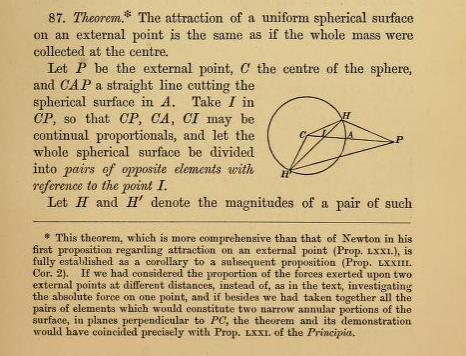
\includegraphics[scale=0.8]{pctrs/1.png}
    \caption{Page 57. from Thomson's
    \href{https://archive.org/details/reprintofpaperso00kelv/page/56/mode/2up?view=theater}{\textit{Reprint
    of papers on electrostatics and magnetism}}}
    \label{ed:thomson:sphericalconductor1}
\end{figure}

\begin{center}
    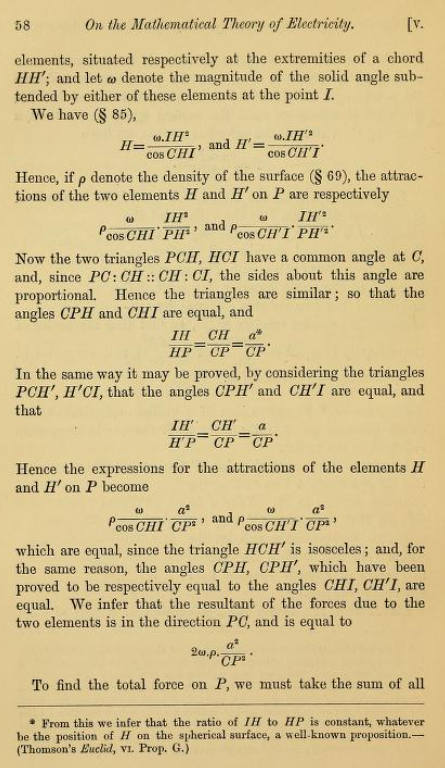
\includegraphics[scale=0.8]{pctrs/2.png}
\end{center}

\textbf{Zadanie.} \textit{Dany jest prostopadłościan o wymiarach \(2a \times a \times a\)
jednorodnie naładowany z gęstości ładunku \(-\rho\) (ładunek ten jest ujemny). Na jednej z jego
dłuższych krawędzi znajduje się bardzo cienka rurka, w której porusza się niewielka kulka o masie m
i ładunku \(q\) (ładunek ten jest dodatni). Kulka wykonuje oscylacje wokół środka krawędzi sześcianu
o amplitudzie dużo mniejszej niż \(a\). Cały układ znajduje się w nieważkości. Wyznacz okres
oscylacji kulki.}
\medskip

\textit{Rozwiązanie.}
\medskip

Rozpatrzmy sześcian o boku \(2a\) jednorodnie naładowany z gęstością ładunku \(\rho\). Obierzmy
kartezjański układ współrzędnych, którego środek pokrywa się ze środkiem symetrii sześcianu, a osie
są równoległe do odpowiednich krawędzi sześcianu. Potencjał w punkcie \(P(0,0,\delta)\) wynosi (dla
ustalenia uwagi przyjmijmy \(q>0\), a więc \(\rho<0\))
\begin{equation*}
\begin{split}
    \varphi(\delta)&=\int_{-a}^a\int_{-a}^a\int_{-a}^a\frac{-k|\rho|}{\sqrt{x^2+y^2+(z-\delta)^2}}\dd{x}\dd{y}\dd{z}\\
    &=-k|\rho| \int_{-a}^a\int_{-a}^a\int_{-a}^a f(\delta)\dd{x}\dd{y}\dd{z}\,.
\end{split}
\end{equation*}
Korzystając ze wzoru Taylora możemy przybliżyć \(f(\delta)\) dla małych \(\delta\) wokół 0
\begin{equation*}
\begin{split}
    f(\delta)&\approx f(0)+f'(0)\delta+\frac{1}{2}f''(0)\delta^2=\\
    &=\frac{1}{\sqrt{x^2+y^2+z^2}}+\frac{z}{(x^2+y^2+z^2)^{3/2}}\delta-\frac{1}{2}\frac{x^2+y^2-2z^2}{(x^2+y^2+z^2)^{5/2}}\delta^2\,.
\end{split}
\end{equation*}
Zauważmy, że wprowadzając funkcję \(g(x,y,z)\) 
\begin{equation*}
    g(x,y,z)=\frac{z}{(x^2+y^2+z^2)^{3/2}}\,,
\end{equation*}
mamy \(f'(0)=g\) i \(f''(0)=-\pdv{g}{z}\). Otrzymujemy więc
\begin{equation*}
\begin{split}
    \varphi(\delta)&=\varphi(0)-k|\rho|\delta \int_{-a}^a\int_{-a}^a\int_{-a}^ag \dd{z}\dd{x}\dd{y}\\
    &+\frac{1}{2}k|\rho|\delta^2\int_{-a}^a\int_{-a}^a\int_{-a}^a\pdv{g}{z}\dd{z}\dd{x}\dd{y}\,.
\end{split}
\end{equation*}
Łatwo zauważyć, że drugi człon jest równy 0, gdyż
\begin{equation*}
    \int_{-a}^a\frac{z}{(A+z^2)^{3/2}}\dd{z}=-\left[\frac{1}{\sqrt{A+z^2}}\right]_{-a}^a=0\,,
\end{equation*}
otrzymujemy zatem potencjał swobodnego oscylatora harmonicznego. Obliczmy zatem całkę
\begin{equation*}
\begin{split}
    &\int_{-a}^a\int_{-a}^a\int_{-a}^a\pdv{g}{z}\dd{z}\dd{x}\dd{y}=\frac{4\pi}{3}\,.
\end{split}
\end{equation*}
Z powyższego więc
\begin{equation*}
    \varphi(\delta)=\varphi(0)+\frac{1}{2}\frac{4\pi k|\rho|}{3}\delta^2\,.
\end{equation*}
Z symetrii i zasady superpozycji potencjałów wynika, że przyczynki do \(\varphi\) od każdego z
prostopadłościanów o wymiarach \(2a\times a \times a\) są takie same i równe \(\varphi/4\), zatem
energia potencjalna \(U(\delta)\) cząstki w naszym zadaniu wynosi
\begin{equation*}
    U(\delta)=U(0)+\frac{1}{2}\frac{k|\rho|\pi q}{3}\delta ^2=U(0)+\frac{1}{2}K \delta^2\,.
\end{equation*}
Jest to energia potencjalna swobodnego oscylatora harmonicznego o okresie \(T\) równym
\begin{equation*}
    T=2\pi\sqrt{\frac{m}{K}}=2\pi\sqrt{\frac{3m}{\pi k |q\rho| }}=2\pi\sqrt{\frac{12m\epsilon_0}{|q\rho| }}\,.
\end{equation*}
\subsubsection{Własności przewodników}
\begin{enumerate}
    \item Wewnątrz przewodnika potencjał jest stały, więc \(\mathbf{E}=0\).
    \item Wewnątrz przewodnika \(\rho=0\).
    \item Na powierzchni przewodnika potencjał jest stały, a pole elektryczne może mieć jedynie
    składową normalną do tej powierzchni w danym punkcie.
    \item Pole elektryczne ma nieciągłość na powierzchni przewodnika, potencjał jest jednak ciągły.
    \item Nieskompensowany ładunek może występować jedynie na powierzchni przewodnik.
\end{enumerate}

\subsubsection{Kondensatory}
Jeśli na dwóch odizolowanych przewodnikach umieścimy ładunki odpowiednio \(Q\) i \(-Q\) to różnica
potencjałów między przewodnikiem naładowanym dodatnio, a przewodnikiem naładowanym ujemnie:
\begin{equation*}
    U=\varphi_+-\varphi_-=-\int_{\mathbf{r}_-}^{\mathbf{r}_+}\mathbf{E}(\mathbf{r}')\cdot\dd{\mathbf{l}}
\end{equation*}
jest proporcjonalna do \(Q\). Stałą proporcjonalności nazywamy \textit{pojemnością} układu
\begin{equation*}
    C=\frac{Q}{U}\,.
\end{equation*}
Obliczmy pojemności następujących układów o wysokiej symetrii:
\begin{enumerate}
    \item Kondensator płaski wykonany z dwóch równoległych płaszczyzn o identycznym kształcie i polu
    powierzchni \(A\) umieszczonych w odległości \(w\ll\sqrt{A}\) od siebie.\\
    Możemy z dobrym przybliżeniem przyjąć, że jeśli płaszczyzny te są naładowane jednorodnie z
    gęstościami odpowiednio \(\sigma\) i \(-\sigma\) to
    \begin{equation*}
        \mathbf{E}(\mathbf{r})=\frac{\sigma \mathbf{\hat{n}}}{\epsilon_0}\quad\text{między płytami i 0 w pozostałym obszarze.}
    \end{equation*}
    Z powyższego zatem
    \begin{equation*}
        U=-\int_w^0\frac{\sigma }{\epsilon_0}\dd{x}=\frac{\sigma w}{\epsilon_0}=\frac{Qw}{\epsilon_0A}\,,
    \end{equation*}
    skąd
    \begin{equation*}
        C=\frac{\epsilon_0 A}{w}\,.
    \end{equation*}
    \item Układ koncentrycznych powłok kulistych o promieniach \(a\) i \(b\) (\(b>a\)) i
    naładowanych odpowiednio ładunkami \(Q\) i \(-Q\). Z prawa Gaussa
    \begin{equation*}
        \mathbf{E}=\begin{cases}
        kQ\mathbf{r}/r^3\quad&\text{dla \(a\leq r\leq b\)}\\
        0\quad&\text{w pozostałym obszarze}
        \end{cases}\,.
    \end{equation*}
    Z powyższego zatem
    \begin{equation*}
        U=-\int_b^a\frac{kQ}{r^2}\dd{r}=\frac{kQ(b-a)}{ab}\,,
    \end{equation*}
    skąd
    \begin{equation*}
        C=\frac{4\pi\epsilon_0ab}{b-a}\,.
    \end{equation*}
    Zauważmy przy tym, że dla \(b\gg a\) otrzymujemy
    \begin{equation*}
        C=4\pi\epsilon_0a\,.
    \end{equation*}
    \item Układ koncentrycznych, długich powłok walcowych o promieniach \(a\) i \(b\), naładowanych
    z gęstościami odpowiednio \(\lambda\) i \(-\lambda\). Z prawa Gaussa mamy
    \begin{equation*}
        \mathbf{E}(s)=\frac{\lambda}{2\pi\epsilon_0 s}\mathbf{\hat{s}}\quad\text{dla \(a<s<b\)}\,,
    \end{equation*}
    skąd
    \begin{equation*}
        U=-\int_b^a\frac{\lambda}{2\pi\epsilon_0s}\dd{s}=\frac{\lambda}{2\pi\epsilon_0}\ln\frac{b}{a}\,.
    \end{equation*}
    Definiując pojemność na jednostkę długości \(\mathcal{C}\) otrzymujemy
    \begin{equation*}
        \mathcal{C}=\frac{\lambda}{U}=\frac{2\pi\epsilon_0}{\ln\frac{b}{a}}\,.
    \end{equation*}
\end{enumerate}
\subsubsection{Energia pola elektrycznego}
Jeśli w pewnym obszarze istnieje pole \(\mathbf{E}\) to w tym obszarze zgromadzona jest energia o
gęstości
\begin{equation*}
    \varkappa_e=\frac{1}{2}\epsilon_0E^2\,.
\end{equation*}
Korzystając z gęstości energii możemy obliczyć energię jaka była potrzebna do stworzenia pewnego
rozkładu ładunków. Rozpatrzmy prosty przykład jednorodnie naładowanej kuli o promieniu \(R\) i
całkowitym ładunku \(Q\):
\begin{equation*}
    \begin{split}
        &\varkappa_e=\begin{cases} \epsilon_0k^2Q^2r^2/2R^6\quad&\text{dla \(r<R\)}\\ \epsilon_0 k^2Q^2/2r^4\quad&\text{dla \(r\geq R\)}\end{cases}\\
        &W=\int_0^\infty\varkappa_e(r)\dd{r}=\frac{3kQ^2}{5R}\,.
    \end{split}
\end{equation*}
Taki sposób liczenia energii działa dobrze do ciągłych rozkładów ładunków. Zauważmy jednak, że
obliczenie w ten sposób energii potrzebnej do stworzenia układu składającego się z pojedynczego
elektronu daje
\begin{equation*}
    W_\text{electron}=\frac{e^2}{8\pi\epsilon_0}\int_0^\infty\frac{\dd{r}}{r^2}=\infty\,.
\end{equation*}
\subsubsection{Dipol elektryczny}
Dipolem elektrycznym nazywamy układ dwóch ładunków \(q\) i \(-q\) znajdujących się w ustalonej
odległości \(d\) od siebie. Gdy \(d>0\) dipol taki nazywamy \textit{dipolem fizycznym} i dla
odległości \(r\gg d\) pole takiego dipola możemy przybliżyć polem tzw. \textit{dipola idealnego}.
Rozpatrzmy dipol fizyczny składający się z dwóch ładunków \(q\), \(-q\) w odległości \(d\) od
siebie. Obierzmy układ współrzędnych kartezjańskich, którego oś \(z\) pokrywa się z osią dipola, a
środek ze środkiem dipola. Układ jest zlokalizowany, więc potencjał \(\varphi(\mathbf{r})\) możemy
obliczyć jako sumę:
\begin{equation*}
    \varphi(\mathbf{r})=\varphi_++\varphi_-=kq\left(\frac{1}{\mathcal{R}_+}+\frac{1}{\mathcal{R}_-}\right)\,.
\end{equation*}
Łatwo zauważyć, że
\begin{equation*}
    \begin{split}
        \mathcal{R}_\pm=\sqrt{r^2+d^2/4\mp rd\cos\theta}\,,
    \end{split}
\end{equation*}
gdzie \(\theta\) jest kątem zenitalnym. Dla \(r\gg d\) możemy przybliżyć
\begin{equation*}
    \mathcal{R}_\pm\approx\sqrt{r^2\mp rd\cos\theta}=r\sqrt{1\mp\frac{d}{r}\cos\theta}\,,
\end{equation*}
korzystając z rozwinięcia Taylora 1-go rzędu mamy zatem
\begin{equation*}
    \frac{1}{\mathcal{R}_\pm}\approx \frac{1}{r}\left(1\pm\frac{d}{2r}\cos\theta\right)\,,
\end{equation*}
czyli
\begin{equation*}
    \varphi(\mathbf{r})=\frac{|\mathbf{p}|}{4\pi\epsilon_0r^2}\cos\theta\quad\text{dla \(r\gg d\)}\,.
\end{equation*}
Dipolem idealnym nazywamy układ, dla którego powyższy wzór jest prawdziwy dla każdego \(r\). Powyżej
wprowadziliśmy elektryczny moment dipolowy \(\mathbf{p}=q\mathbf{d}\). Mając potencjał możemy
obliczyć natężenie pola \(\mathbf{E}\) generowanego przez idealny dipol
\begin{equation*}
    \mathbf{E}_\text{dip}(\mathbf{r})=\frac{|\mathbf{p}|}{4\pi\epsilon_0r^3}(2\cos\theta\mathbf{\hat{r}}+\sin\theta\boldsymbol{\hat{\theta}})\,.
\end{equation*}
Jeśli idealny dipol \(\mathbf{p}\) umieścimy w zewnętrznym polu \(\mathbf{E}\) to można pokazać, że:
posiada on energię \(W\)
\begin{equation*}
    W=-\mathbf{p}\cdot\mathbf{E}\,,
\end{equation*}
działa na niego moment siły \(\boldsymbol{\Gamma}\)
\begin{equation*}
    \boldsymbol{\Gamma}=\mathbf{p}\times\mathbf{E}
\end{equation*}
oraz siła \(\mathbf{F}\)
\begin{equation*}
    \mathbf{F}=\nabla(\mathbf{p\cdot\mathbf{E}})\,.
\end{equation*}
\subsubsection{Pola elektryczne w materii}
Jeśli kawałek dielektryka umieścimy w zewnętrznym polu \(\mathbf{E}\) to wewnątrz dielektryka
indukuje się wiele małych dipoli, skierowanych zgodnie z kierunkiem pola -- materiał zostaje
spolaryzowany. Definiujemy wektor polaryzacji  elektrycznej \(\mathbf{P}\)
\begin{equation*}
    \mathbf{P}=\dv{\mathbf{p}}{V}
\end{equation*}
określający elektryczny moment dipolowy na jednostkę objętości substancji. Ponieważ w materiale
pojawia się wiele małych dipoli to indukuje się również pewien ładunek, który nazywamy
\textit{związanym}. Jego gęstość objętościowa i powierzchniowa wynoszą odpowiednio
\begin{equation*}
    \rho_\text{zw}=-\nabla\cdot\mathbf{P}\quad\text{oraz}\quad \sigma_\text{zw}=\mathbf{P}\cdot\mathbf{\hat{n}}\,.
\end{equation*}
Pole elektryczne wytwarzane przez spolaryzowaną materię jest więc takie, jak od ładunku związanego o
gęstości powierzchniowej \(\sigma_\text{zw}\) i objętościowej \(\rho_\text{zw}\). Jeśli w pewnej
przestrzeni znajdują się zarówno ładunki związane i ładunki swobodne, które razem generują wypadkowe
pole \(\mathbf{E}\) to z prawa Gaussa mamy
\begin{equation*}
    \epsilon_0\nabla\cdot\mathbf{E}=\rho=\rho_\text{sw}+\rho_\text{zw}=\rho_\text{sw}-\nabla\cdot\mathbf{P}\,,
\end{equation*}
zatem wprowadzając wektor \(\mathbf{D}=\epsilon_0\mathbf{E}+\mathbf{P}\) (przesunięcia
elektrycznego) mamy
\begin{equation*}
    \nabla\cdot\mathbf{D}=\rho_\text{sw}\,.
\end{equation*}
Z tw. Greena możemy podać równoważną postać
\begin{equation*}
    \oint_\mathcal{S}\mathbf{D}\cdot\dd{\mathbf{S}}=Q_\text{sw}\,,
\end{equation*}
gdzie \(Q_\text{sw}\) jest całkowitym swobodnym, tj. niezwiązanym z materią dielektryka, ładunkiem
zawartym w przestrzeni ograniczonej powierzchnią zamkniętą \(\mathcal{S}\). Równanie to nie jest
żadnym nowym prawem, a jedynie sprytnym podzieleniem gęstości ładunku na część swobodną i związaną z
polaryzowaną materią. Zauważmy jednocześnie, że powyższe równanie nie wyznacza pola \(\mathbf{D}\)
jednoznacznie, gdyż znamy tylko jego dywergencją, natomiast rotacja (w elektrostatyce) wynosi
\begin{equation*}
    \nabla\times\mathbf{D}=\nabla\times\mathbf{P}\,,
\end{equation*}
co w ogólności jest różne od 0 i musimy znać jawną postać \(\mathbf{P}(\mathbf{r})\), aby wyznaczyć
pole \(\mathbf{D}\).
\subsubsection*{Dielektryki liniowe}
Dla izotropowych i jednorodnych dielektryków liniowych zachodzi
\begin{equation*}
    \mathbf{P}=\epsilon_0\chi_e\mathbf{E}\,,
\end{equation*}
gdzie \(\mathbf{E}\) jest \textbf{wypadkowym} polem elektrycznym pochodzącym zarówno od ładunków
swobodnych jak i związanej materii, a \(\chi_e\) to tzw. \textit{podatność elektryczna}. W takim
przypadku zachodzi
\begin{equation*}
    \mathbf{D}=\epsilon_0(1+\chi_e)\mathbf{E}=\epsilon_0\epsilon_r\mathbf{E}\,.
\end{equation*}
\subsubsection*{Zadania.}
\begin{enumerate}
    \item \textit{Znaleźć pole \(\mathbf{E}\) pochodzące od jednorodnie spolaryzowanej kuli o
    polaryzacji \(\mathbf{P}\)}.
\medskip

\noindent W przypadku jednorodnie spolaryzowanej kuli mamy tak naprawdę do czynienia z dwiema kulami
ładunku, które się przenikają. Korzystając z wyników zadania o dwóch przekrywających się kulach mamy
\begin{equation*}
    \mathbf{E}=-\frac{\rho}{3\epsilon_0}\mathbf{d}\,,
\end{equation*}
w środku kuli i pole idealnego dipola umieszczonego na zewnątrz. Moment dipolowy wynosi
\begin{equation*}
    \mathbf{p}=\frac{4}{3}\pi R^3\rho\mathbf{d}=\frac{4}{3}\pi R^3\mathbf{P}\,.
\end{equation*}
Mamy zatem
\begin{equation*}
    \mathbf{E}=\begin{cases} -\mathbf{P}/3\epsilon_0&\quad\text{wewnątrz kuli}\\ \mathbf{E}_\text{dip}&\quad\text{na zewnąrz kuli}\end{cases}\,.
\end{equation*}

\item \textit{Kula wykonana z jednorodnego, izotropowego i liniowego dielektryka o podatności
\(\chi\) została umieszczona w jednorodnym zewnętrznym polu \(\mathbf{E}_0\). Znaleźć natężenie
pola.}
\medskip

\noindent Polaryzacja kuli będzie jednorodna, zatem
\begin{equation*}
    \mathbf{E}_\text{in}=\mathbf{E}_0-\frac{1}{3\epsilon_0}\mathbf{P}
\end{equation*}
oraz mamy
\begin{equation*}
    \mathbf{P}=\epsilon_0\chi\mathbf{E}_\text{in}\,,
\end{equation*}
skąd otrzymujemy
\begin{equation*}
    \mathbf{E}_\text{in}=\left(\frac{3}{\chi+3}\right)\mathbf{E}_0\,.
\end{equation*}
Na zewnątrz mamy natomiast
\begin{equation*}
    \mathbf{E}_\text{out}(\mathbf{r})=\mathbf{E}_0+\frac{|\mathbf{p}|}{4\pi\epsilon_0r^3}(2\cos\theta\mathbf{\hat{r}}+\sin\theta\boldsymbol{\hat{\theta}})\,,
\end{equation*}
gdzie
\begin{equation*}
    |\mathbf{p}|=\frac{4}{3}\pi R^3|\mathbf{P}|=\left(\frac{\chi}{\chi+3}\right)4\pi\epsilon_0R^3|\mathbf{E}_0|\,.
\end{equation*}
W granicznym przypadku, w którym dielektryk przechodzi w przewodnik tj. \(\chi\to\infty\)
otrzymujemy
\begin{equation*}
    \begin{split}
        &\mathbf{E}_\text{in}=0\\
        &\mathbf{E}_\text{out}=\mathbf{E}_0+\frac{R^3}{r^3}|\mathbf{E}_0|(2\cos\theta\mathbf{\hat{r}}+\sin\theta\boldsymbol{\hat{\theta}})\,.
    \end{split}
\end{equation*}
\end{enumerate}

\subsubsection{Równanie Poissona i Laplace'a}
Podstawiając \(\mathbf{E}=-\nabla\varphi\) do prawa Gaussa otrzymujemy tzw. równanie Poissona
\begin{equation*}
    \nabla ^2\varphi+\frac{\rho}{\epsilon_0}=0\,,
\end{equation*}
będące naszym centralnym zainteresowaniem w elektrostatyce, gdyż jego rozwiązaniem dla zadanego
rozkładu \(\rho(\mathbf{r})\) jest potencjał elektryczny. Jeśli w interesującym nas obszarze
\(\rho=0\), wówczas otrzymujemy równanie Laplace'a
\begin{equation*}
    \nabla^2\varphi=0\,.
\end{equation*}

\noindent\fbox{%
    \parbox{\linewidth}{%
        \textbf{Twierdzenie o jednoznaczności}\\
    Rozwiązanie równania Poissona w pewnym obszarze \(\mathcal{V}\) jest określone jednoznacznie,
    jeśli podana jest wartość rozwiązania \(\varphi\) na powierzchni \(\mathcal{S}\) będącej
    brzegiem obszaru \(\mathcal{V}\), przy czym dopuszczalne jest, aby w \(\mathcal{V}\) znajdowały
    się \textit{wyspy} o ile \(\varphi\) jest zadane również na wszystkich powierzchniach je
    ograniczających.
        
    }%
}\\
\subsubsection{Warunki brzegowe w elektrostatyce}
Niech \(\mathcal{S}\) oznacza brzeg pewnego obszaru \(\mathcal{V}\). Wówczas warunki brzegowe na
powierzchni \(\mathcal{S}\) mają postać:
\begin{itemize}
    \item \(E_\text{nad}^\parallel-E_\text{pod}^\parallel=0\)
    \item \(D_\text{nad}^\perp-D_\text{pod}^\perp=\sigma_\text{sw}\)\,,
\end{itemize}
gdzie indeksy \textit{nad} i \textit{pod} oznaczają, że bierzemy odpowiednio składowe równoległe lub
prostopadłe do powierzchni \(\mathcal{S}\) tuż nad lub tuż pod tą powierzchnią. Dla izotropowego,
jednorodnego i liniowego ośrodka o względnej przenikalności elektrycznej \(\epsilon\) umieszczonego
w próżni, dla którego \(\sigma_\text{sw}=0\), zachodzi
\begin{equation*}
    \pdv{\varphi_o}{n}=\epsilon\pdv{\varphi_i}{n}\,,\quad\quad \varphi_i=\varphi_o\,.
\end{equation*}
Jeśli \(\mathcal{S}\) jest brzegiem przewodnika to drugi warunek możemy zapisać jako
\begin{equation*}
    \sigma(\mathbf{r})=-\epsilon_0\pdv{\varphi}{n}\Big|_\mathcal{S}\,,
\end{equation*}
gdzie \(\mathbf{\hat{n}}\) jest wersorem normalnym do \(\mathcal{S}\). Siła na jednostkę powierzchni
działająca na \(\mathcal{S}\) wynosi
\begin{equation*}
    \mathbf{f}=\frac{\sigma}{2}(\mathbf{E}_\text{nad}+\mathbf{E}_\text{pod})\,,
\end{equation*}
siła na jednostkę objętości działająca na \(\mathcal{V}\) wynosi
\begin{equation*}
    \mathbf{f}(\mathbf{r})=\rho(\mathbf{r})\mathbf{E}(\mathbf{r})\,.
\end{equation*}
\subsubsection{Metoda obrazów}
Na tw. o jednoznaczności opiera się jedna z najładniejszych metod rozwiązywania równania Poissona w
szczególnych przypadkach. Metoda ta działa w ogólności, nie tylko w elektrostatyce. Wystarczy bowiem
zgadnąć funkcję \(\varphi\), która spełnia wszystkie warunki brzegowe, a twierdzenie o
jednoznaczności gwarantuje nam, że jest to właściwe (i jedyne) rozwiązanie. Często okazuje się, że
dany układ jest w pewnym sensie równoważny układowi złożonemu ze skończonej liczby ładunków
punktowych.
\subsubsection*{Zadania}
\begin{enumerate}
    \item \textit{Ładunek punktowy umieszczony nad nieskończoną przewodzącą płaszczyzną}
    \medskip
    
    Jedynymi warunkami brzegowymi są tutaj: \(\varphi(x,y,0)=0\), \(\varphi(\infty)=0\) i ładunek
    \(q\) umieszczony w \((0,0,d)\). Warunki te można spełnić umieszczając ładunek obrazowy \(-q\) w
    \((0,0,-d)\). Wówczas potencjał dla \(z>0\) spełnia wszystkie warunki brzegowe i nie zmieniliśmy
    rozkładu dla \(z>0\), zatem z tw. o jednoznaczności jest to właściwy potencjał. Potencjał dla
    \(z>0\) ma więc postać
    \begin{equation*}
        \varphi(\mathbf{r})=\frac{kq}{\sqrt{x^2+y^2+(z-d)^2}}-\frac{kq}{\sqrt{x^2+y^2+(z+d)^2}}\,.
    \end{equation*}
    Dla \(z<0\) oczywiście \(\varphi=0\). Gęstość powierzchniowa indukowanego ładunki wynosi
    natomiast
    \begin{equation*}
        \sigma(\mathbf{r})=-\epsilon_0\pdv{\varphi}{z}\Big|_{z=0}=\frac{1}{2\pi}\frac{-qd}{(x^2+y^2+d^2)^{3/2}}\,.
    \end{equation*}
    Siła działająca na \(q\) wynosi
    \begin{equation*}
        \mathbf{F}(d)=-\frac{kq^2}{4d^2}\mathbf{\hat{z}}\,.
    \end{equation*}
    Energia takiego układu wynosi więc
    \begin{equation*}
        U=-\int_\infty^d F_z(z')\cdot\dd{z'}=-\frac{kq^2}{4d}\,.
    \end{equation*}
    
    \item \textit{Ładunek punktowy umieszczony między dwiema prostopadłymi półpłaszczyznami}
    \medskip
    
    Warunkami brzegowymi są: \(\varphi(0,y,z)=0\), \(\varphi(x,0,z)=0\), \(\varphi(\infty)=0\) oraz
    ładunek \(q\) umieszczony w \((b,a,0)\). Łatwo sprawdzić, że potencjał
    \begin{equation*}
        \varphi(\mathbf{r})=\frac{q}{4\pi\epsilon_0}\left(\frac{1}{\varsigma_1}-\frac{1}{\varsigma_2}+\frac{1}{\varsigma_3}-\frac{1}{\varsigma_4}\right)\,,
    \end{equation*}
    gdzie
    \begin{equation*}
        \begin{split}
            &\varsigma_1=\sqrt{(a-x)^2+(b-y)^2}\\
            &\varsigma_2=\sqrt{(a+x)^2+(b-y)^2}\\
            &\varsigma_3=\sqrt{(a+x)^2+(b+y)^2}\\
            &\varsigma_4=\sqrt{(a-x)^2+(b+y)^2}\,,
        \end{split}
    \end{equation*}
    spełnia zadane warunki brzegowe, zatem z tw. o jednoznaczności jest to właściwy potencjał. Jest
    to oczywiście potencjał generowany przez układ czterech ładunków \(q,-q,q,-q\) umieszczonych w
    wierzchołkach prostokąta o bokach \(2a\) i \(2b\). Siła działająca na ładunek \(q\) wynosi
    \begin{equation*}
        \mathbf{F}(b,a)=\frac{q^2}{16\pi\epsilon_0}\left[\mathbf{\hat{x}}\left(\frac{b}{(a^2+b^2)^{3/2}}-\frac{1}{b^2}\right)+\mathbf{\hat{y}}\left(\frac{a}{(a^2+b^2)^{3/2}}-\frac{1}{a^2}\right)\right]\,.
    \end{equation*}
    Energia układu wynosi natomiast
    \begin{equation*}
    \begin{split}
        U&=-\int_\infty^x F_x(x',\infty)\dd{x'}-\int_\infty^yF_y(x,y')\dd{y'}\\
        &=-\frac{q^2}{16\pi\epsilon_0}\left(\frac{1}{x}+\frac{1}{y}-\frac{1}{\sqrt{x^2+y^2}}\right)\,.
    \end{split}
    \end{equation*}
    Okazuje się, że skończoną liczbę ładunków obrazowych można uzyskać tylko dla półpłaszczyzn
    ustawionych pod kątem \(\alpha\) takim, że \(\pi=n\alpha\), gdzie \(n\in\mathbb{Z}_+\). Liczba
    potrzebnych ładunków obrazowych wynosi wówczas \(2\pi/\alpha -1\).
    
    \item \textit{Ładunek punktowy umieszczony nad półprzestrzenią wypełnioną dielektrykiem o
    podatności \(\chi\)}
    \medskip
    
    Zakładając liniowy, jednorodny i izotropowy dielektryk warunki brzegowe na powierzchni
    granicznej mają postać
    \begin{equation*}
        \pdv{\varphi}{z}\bigg|_{z=0^+}=(1+\chi)\pdv{\varphi}{z}\bigg|_{z=0^-}\,,\quad \varphi(x,y,0^+)=\varphi(x,y,0^-)\,,
    \end{equation*}
    gdzie równości zachodzą dla wszystkich \(x\), \(y\). Poszukajmy rozwiązań w postaci superpozycji
    potencjałów ładunków punktowych
    \begin{equation*}
        \begin{split}
            &\varphi_1(x,y,z)=\frac{q}{4\pi\epsilon_0}\frac{1}{\sqrt{x^2+y^2+(z-d)^2}}+\frac{q'}{4\pi\epsilon_0}\frac{1}{\sqrt{x^2+y^2+(z+d)^2}}\,,\\
            &\varphi_2(x,y,z)=\frac{q''}{4\pi\epsilon_0}\frac{1}{\sqrt{x^2+y^2+(z-d)^2}}\,,
        \end{split}
    \end{equation*}
    gdzie \(\varphi_1\) określa potencjał dla \(z>0\), a \(\varphi_2\) dla \(z<0\). Z warunku
    ciągłości potencjału mamy
    \begin{equation*}
        q+q'=q''\,,
    \end{equation*}
    natomiast z drugiego warunku mamy
    \begin{equation*}
        q-q'=(1+\chi)q''\,,
    \end{equation*}
    skąd otrzymujemy
    \begin{equation*}
        q'=-\left(\frac{\chi}{\chi+2}\right)q\,,\quad q''=\left(\frac{2}{\chi+2}\right)q\,.
    \end{equation*}
    Dla podanych wartości ładunków \(q'\) i \(q''\) powyższy potencjał spełnia wszystkie warunki
    brzegowe (łącznie z \(\varphi(r\to\infty)=0\)), zatem z tw. o jednoznaczności jest to właściwy
    potencjał. Możemy zatem wyznaczyć rozkład \(\sigma_\text{zw}(\mathbf{r})\) ładunku na
    powierzchni dielektryka
    \begin{equation*}
        \sigma_\text{zw}(x,y)=-\epsilon_0\left(\pdv{\varphi_1}{z}\bigg|_{z=0^+}-\pdv{\varphi_2}{z}\bigg|_{z=0^-}\right)=\frac{1}{2\pi}\left(\frac{\chi}{\chi+2}\right)\frac{-qd}{(x^2+y^2+d^2)^{3/2}}\,.
    \end{equation*}
   Siła działająca na ładunek wynosi natomiast
    \begin{equation*}
        \mathbf{F}=-\left(\frac{\chi}{\chi+2}\right)\frac{kq^2}{4d^2}\mathbf{\hat{z}}\,.
    \end{equation*}
    
    \item\textit{Dwie przewodzące rury}
    \medskip
    
    Rozpatrzmy dwie nieskończone przewodzące rury o promieniach \(a\), których środki są oddalone o
    \(2d\). Pierwsza rura ma potencjał \(-V_0\) względem pewnego punktu odniesienia, a druga
    \(+V_0\). Pokażemy, że takie powierzchnie ekwipotencjalne można uzyskać dla układu dwóch
    naładowanych nici \(-\lambda\) i \(+\lambda\) oddalonych o \(2b\) oraz wyznaczymy odpowiednie
    \(\lambda\) i \(b\). Istotnie rozpatrzmy dwie naładowane nici. Przyjmując początek układu
    współrzędnych w połowie między nimi z osią \(z\) skierowaną prostopadle do wyznaczonej przez nie
    płaszczyzny mamy
    \begin{equation*}
        \varphi=-\frac{\lambda}{2\pi\epsilon_0}\ln\frac{s_+}{C}+\frac{\lambda}{2\pi\epsilon_0}\ln\frac{s_-}{C}=\frac{\lambda}{2\pi\epsilon_0}\ln\frac{s_-}{s_+}\,.
    \end{equation*}
    Jednocześnie
    \begin{equation*}
        s_\pm=\sqrt{(y\mp b)^2+z^2}\,,
    \end{equation*}
    zatem
    \begin{equation*}
        \varphi(\mathbf{r})=\frac{\lambda}{4\pi\epsilon_0}\ln\frac{(y+b)^2+z^2}{(y-b)^2+z^2}\,.
    \end{equation*}
    Musimy znaleźć rozwiązanie równania
    \begin{equation*}
        K=\frac{(y+b)^2+z^2}{(y-b)^2+z^2}\,,
    \end{equation*}
    gdzie \(K=\exp(4\pi\epsilon_0V_0/\lambda)\). Przekształcając otrzymujemy
    \begin{equation*}
        y^2-2b\left(\frac{K+1}{K-1}\right)y+b^2+z^2=0\,.
    \end{equation*}
    Równanie okręgu ma postać
    \begin{equation*}
        y^2-2yy_0+y_0^2-R^2+z^2=0\,.
    \end{equation*}
    Porównując te wyrażenia otrzymujemy
    \begin{equation*}
        \begin{split}
            &y_0=b\left(\frac{K+1}{K-1}\right)=b\coth\frac{2\pi\epsilon_0V_0}{\lambda}\\
            &R=\sqrt{y_0^2-b^2}\,.
        \end{split}
    \end{equation*}
    Znając \(R=a\) i \(y_0=d\) możemy wyznaczyć \(b\) i \(\lambda\)
    \begin{equation*}
    \begin{split}
        &\lambda=\frac{2\pi\epsilon_0V_0}{\cosh^{-1}{(d/a)}}\\
        &b=\sqrt{d^2-a^2}\,.
    \end{split}
    \end{equation*}
    Potencjał w całej przestrzeni wynosi więc
    \begin{equation*}
        \varphi(\mathbf{r})=\frac{V_0}{2\cosh^{-1}(d/a)}\ln\left\{\frac{(y+\sqrt{d^2-a^2})^2+z^2}{(y-\sqrt{d^2-a^2})^2+z^2}\right\}\,.
    \end{equation*}
    
    \item \textit{Przewodzący, cienki dysk}
    \medskip
    
    Chcemy wyznaczyć gęstość powierzchniową ładunku \(\sigma\) na cienkim metalowym dysku o
    promieniu \(R\) umieszczonym w pustej przestrzeni, na którym utrzymywany jest stały potencjał
    \(V_0\) (lub dysk naładowany jest całkowitym ładunkiem \(Q\)). Oczywiście ze względu na symetrię
    \(\sigma\) może zależeć tylko od współrzędnej radialnej \(s\).
    \medskip
    
    Udowodnimy następujące twierdzenie: rozkład ładunku na powierzchni odosobnionego, metalowego
    dysku naładowanego ładunkiem \(Q\) jest taki, że infinitezymalny ładunek \(\dd{q}=\sigma
    \dd{S}\) znajdujący się w punkcie \(X\) na powierzchni dysku jest równy ładunkowi znajdującemu
    się w punkcie przecięcia prostej prostopadłej do płaszczyzny dysku przechodzącej przez \(X\) z
    naładowaną jednorodnie z gęstością powierzchniową \(\sigma_0=Q/4\pi R^2\) sferą, której kołem
    wielkim jest ów dysk. Istotnie rozpatrzmy dowolny punkt \(P\) na kole wielkim \(AB\) naładowanej
    sfery oraz dowolną cięciwę \(CD\) sfery zawierającą \(P\). Infinitezymalny ładunek zgromadzony w
    \(C\) i \(D\) wynosi odpowiednio
    \begin{equation*}
        \dd{q}_C=\sigma_0\dd{S}_C\,,\quad \dd{q}_D=\sigma_0\dd{S}_D\,,
    \end{equation*}
    gdzie \(\dd{S}_C\), \(\dd{S}_D\) są infitezymalnymi fragmentami powierzchni sfery otaczającymi
    odpowiednio punkt \(C\) i \(D\). W granicy zachodzi
    \begin{equation*}
        \frac{\dd{S}_C}{\dd{S_D}}=\frac{PC^2}{PD^2}\,.
    \end{equation*}
    Rozpatrzmy teraz osobną sytuację, w której mamy cienki dysk \(AB\) naładowany w taki sposób, że
    \(\dd{q}_{C'}=\dd{q}_C\) i \(\dd{q}_{D'}=\dd{q}_D\), gdzie \(C'\), \(D'\) są rzutami
    prostokątnymi punktów \(C\), \(D\) na koło wielkie \(AB\). Oczywiście całkowity ładunek dysku
    wynosi wówczas \(Q\). Pole elektryczne w punkcie \(P\) pochodzące od ładunków \(\dd{q}_{C'}\) i
    \(\dd{q}_{D'}\) wynosi
    \begin{equation*}
        \frac{k\sigma_0\dd{S}_C}{C'P^2}-\frac{k\sigma_0\dd{S}_D}{D'P^2}=k\sigma_0\dd{S}_D\left(\frac{PC^2}{PD^2\cdot C'P^2}-\frac{1}{D'P^2}\right)\,.
    \end{equation*}
    
    \begin{figure}[ht]
    \centering
    \begin{tikzpicture}[line cap=round,line join=round,>=triangle 45,x=1cm,y=1cm,scale=0.7]
\clip(-17,8) rectangle (-7,18); \draw [shift={(-11.790134107302215,13.171364848763671)},line
width=0pt] (0,0) -- (123.55925804040555:0.39144749639608173) arc
(123.55925804040555:162.32882180271702:0.39144749639608173) -- cycle; \draw [line width=0.4pt]
(-11.790134107302215,13.171364848763671) circle (4.236654832859354cm); \draw [line width=0.4pt]
(-15.078357285291432,14.218948455633742)-- (-14.332367964179264,16.560507983796263); \draw [line
width=0.4pt] (-14.332367964179264,16.560507983796263)-- (-10.644735402281466,9.092479464332367);
\draw [line width=0.4pt] (-10.644735402281466,9.092479464332367)--
(-9.57054040469577,12.464232196598486); \draw [line width=0.4pt,dashed]
(-14.13215323265367,16.70183090713026)-- (-10.983038924500262,9.012297460671915); \draw [line
width=0.4pt,dashed] (-10.348392018535602,9.187569683061824)--
(-14.500268036077266,16.427807426315567); \draw [line width=0.4pt,dashed]
(-14.500268036077266,16.427807426315567)-- (-15.192405184725748,14.25528257998549); \draw [line
width=0.4pt,dashed] (-14.937466207955822,14.17406245642328)--
(-14.13215323265367,16.70183090713026); \draw [line width=0.4pt,dashed]
(-10.983038924500262,9.012297460671915)-- (-9.854479906346574,12.554691496704184); \draw [line
width=0.4pt,dashed] (-10.348392018535602,9.187569683061824)--
(-9.329006537384975,12.387282760321643); \draw [line width=0.4pt]
(-15.826879416607003,14.45741752287788)-- (-7.753388797997426,11.885312174649465); \draw [line
width=0.4pt] (-11.790134107302215,13.171364848763671)-- (-14.13215323265367,16.70183090713026);
\begin{scriptsize}
\draw [fill=black] (-11.790134107302215,13.171364848763671) circle (1.5pt); \draw[color=black]
(-11.409055341311891,13.460258566002118) node {$O$}; \draw [fill=black]
(-7.753388797997426,11.885312174649465) circle (1.5pt); \draw[color=black]
(-7.494580377351073,11.803130831258711) node {$B$}; \draw [fill=black]
(-15.826879416607003,14.45741752287788) circle (1.5pt); \draw[color=black]
(-16.30214904626291,14.634601055190359) node {$A$}; \draw [fill=black]
(-12.819817049971508,13.497357527550303) circle (1.5pt); \draw[color=black]
(-12.70083207941896,13.877802562157937) node {$P$}; \draw [fill=black]
(-14.332367964179264,16.560507983796263) circle (1.5pt); \draw[color=black]
(-14.42320106356172,16.878900034527888) node {$C$}; \draw [fill=black]
(-10.644735402281466,9.092479464332367) circle (1.5pt); \draw[color=black]
(-10.600063848759989,8.762888609249154) node {$D$}; \draw [fill=black]
(-15.078357285291432,14.218948455633742) circle (1.5pt); \draw[color=black]
(-15.114758307194798,13.877802562157937) node {$C'$}; \draw [fill=black]
(-9.57054040469577,12.464232196598486) circle (1.5pt); \draw[color=black]
(-9.373528360052266,12.860039071528128) node {$D'$}; \draw [color=black]
(-9.329006537384975,12.387282760321643)-- ++(-1.5pt,0 pt) -- ++(3pt,0 pt) ++(-1.5pt,-1.5pt) -- ++(0
pt,3pt); \draw [color=black] (-9.854479906346574,12.554691496704184)-- ++(-1.5pt,0 pt) -- ++(3pt,0
pt) ++(-1.5pt,-1.5pt) -- ++(0 pt,3pt); \draw [color=black] (-15.192405184725748,14.25528257998549)--
++(-1.5pt,0 pt) -- ++(3pt,0 pt) ++(-1.5pt,-1.5pt) -- ++(0 pt,3pt); \draw [color=black]
(-14.937466207955822,14.17406245642328)-- ++(-1.5pt,0 pt) -- ++(3pt,0 pt) ++(-1.5pt,-1.5pt) -- ++(0
pt,3pt); \draw[color=black] (-12.73997682905857,15.20872404990461) node {$R$}; \draw[color=black]
(-12.2,13.45) node {$\theta$};
\end{scriptsize}
\end{tikzpicture}
    \caption{Konstrukcja poszukiwanego rozkładu \(\sigma\)}
    \label{fig:discproof}
\end{figure}
Z podobieństwa trójkątów \(\Delta C'CP\) i \(\Delta D'DP\) mamy
\begin{equation*}
        \frac{C'P}{CP}=\frac{D'P}{DP}\,,
\end{equation*}
skąd otrzymujemy
\begin{equation*}
    \frac{k\sigma_0\dd{S}_C}{C'P^2}-\frac{k\sigma_0\dd{S}_D}{D'P^2}=k\sigma_0\dd{S}_D\left(\frac{PC^2}{PD^2\cdot C'P^2}-\frac{1}{D'P^2}\right)=0\,.
\end{equation*}
Powtarzając konstrukcję dla wszystkich punktów dysku (po obu jego stronach) otrzymujemy
\(\mathbf{E}(P)=0\), ale punkt \(P\) wybraliśmy dowolnie, zatem dla każdego punktu \(P\) należącego
do dysku \(\mathbf{E}(P)=0\), więc potencjał wewnątrz dysku jest stały. Zauważmy jednak, że w ten
sposób spełniliśmy wszystkie warunki brzegowe zagadnienia metalowego dysku naładowanego ładunkiem
\(Q\) i umieszczonego w pustej przestrzeni tj. potencjał w obszarze dysku jest stały, a całkowity
ładunek wynosi \(Q\). Z tw. o jednoznaczności skonstruowany rozkład jest zatem poszukiwanym
rozkładem dla metalowego dysku. Pozostaje wyznaczyć \(\sigma(C')\). Mamy
\begin{equation*}
    \sigma(C')\dd{S}_{C'}=\sigma_0\dd{S}_C
\end{equation*}
oraz
\begin{equation*}
    \dd{S}_{C'}=\dd{S}_C\frac{CC'}{R}=\dd{S}_C\frac{\sqrt{R^2-OC'^2}}{R}\,.
\end{equation*}
Z powyższego otrzymujemy zatem
\begin{equation*}
    \sigma(C')=\frac{\sigma_0R}{\sqrt{R^2-OC'^2}}=\frac{Q}{4\pi R}\frac{1}{\sqrt{R^2-OC'^2}}
\end{equation*}
po każdej stronie dysku. Oznaczając \(OC'=s\) mamy 
\begin{equation*}
    \sigma(s)=\frac{Q}{4\pi R}\frac{1}{\sqrt{R^2-s^2}}\,.
\end{equation*}
Potencjał \(V_0\) możemy znaleźć wykonując elementarne całkowanie. Przyjmując
\(\varphi(r\to\infty)=0\) mamy
\begin{equation*}
    V_0=2\int_0^{2\pi}\int_0^R\frac{k\sigma(s)}{s}s\dd{s}\dd{\phi}=\frac{Q}{8\epsilon_0R}\,,
\end{equation*}
zatem
\begin{equation*}
    \sigma(s)=\frac{2\epsilon_0V_0}{\pi}\frac{1}{\sqrt{R^2-s^2}}\,.
\end{equation*}
Pojemność metalowego dysku o promieniu \(R\) wynosi z powyższego
\begin{equation*}
    C_\text{disc}=\frac{Q}{V_0}=8\epsilon_0 R\,,
\end{equation*}
jednocześnie pojemność metalowej sfery o promieniu \(R\) wynosi
\begin{equation*}
    C_\text{sphere}=\frac{Q}{V_0}=\frac{4\pi\epsilon_0 RV_0}{V_0}=4\pi\epsilon_0R\,.
\end{equation*}
Stosunek tych pojemności wynosi 
\begin{equation*}
    \frac{C_\text{sphere}}{C_\text{disc}}=\frac{\pi}{2}\,.
\end{equation*}
Ten stosunek został wyznaczony doświadczalnie przez H. Cavendisha, który otrzymał wartość \(1.57\).
\item \textit{Przewodząca wydłużona sferoida}

\medskip
Metoda obrazów jest niezwykle elementarnym, acz potężnym narzędziem. Można jednak odnieść wrażenie,
iż poza typowymi układami, które znajdziemy w każdym podręczniku nie ma ona większych zastosowań.
Poniżej przedstawiamy mało popularny układ, który daje się rozwiązać bez zaawansowanych metod
matematycznych. Rozpatrzmy metalową powłokę w kształcie elipsoidy obrotowej danej równaniem
\begin{equation*}\label{eq:spheroid}
    \frac{z^2}{a^2}+\frac{x^2+y^2}{b^2}=1\,,
\end{equation*}
gdzie zakładamy \(a\geq b\), tzn. elipsoida jest wydłużona. Niech \(A\), \(B\) oznaczają ogniska tej
elipsoidy. Załóżmy, że rozpatrywany przewodnik został umieszczony w próżni z dala od innych ładunków
i jest na nim utrzymywany potencjał \(V_0\) względem nieskończoności. Wyznaczymy potencjał w
dowolnym punkcie na zewnątrz elipsoidy. W myśl metody obrazów rozpatrzmy inny układ, w którym dany
jest odcinek \(AB\) naładowany jednorodnie z gęstością liniową ładunku \(\lambda\). Pokażemy, że dla
takiego układu powierzchnie ekwipotencjalne są wydłużonymi elipsoidami obrotowymi. Istotnie
rozpatrzmy dowolny punkt \(S\in AB\) oraz dowolny punkt \(P\notin AB\). Przyczynek do potencjału w
punkcie \(P\) od punktu \(S\) wynosi
\begin{equation*}
    \dd V=\frac{1}{4\pi\epsilon_0}\frac{\lambda \dd{x}}{SP}\,,
\end{equation*}
gdzie \(\dd{x}\) jest infinitezymalnym fragmentem odcinka \(AB\). Z tw. Stewarta w trójkącie
\(\Delta APB\) mamy natomiast
\begin{equation*}
    SP=\frac{1}{\sqrt{AB}}\sqrt{(AB-x)(AP^2-AB\,x)+BP^2x}\,,
\end{equation*}
gdzie \(x=AS\). Z powyższego zatem
\begin{equation*}
    V(P)=\frac{\lambda \sqrt{AB}}{4\pi\epsilon_0}\int_0^{AB}\frac{\dd{x}}{\sqrt{(AB-x)(AP^2-AB\,x)+BP^2x}}\,.
\end{equation*}
Wynikiem powyższej całki jest
\begin{equation*}
    V(P)=\frac{\lambda}{4\pi\epsilon_0}\log\left\{\frac{AP+BP+AB}{AP+BP-AB}\right\}\,.
\end{equation*}
Powierzchnie ekwipotencjalne są dane równaniem \(V(P)=V_0\), skąd po przekształceniach otrzymujemy
\begin{equation*}
    AP+BP=AB\,\coth\left\{\frac{2\pi\epsilon_0V_0}{\lambda}\right\}=\text{const.}
\end{equation*}
Zbiór punktów przestrzeni, których suma odległości od dwóch ustalonych punktów \(A\), \(B\) jest
stała to wydłużona elipsoida obrotowa. Potencjał w dowolnym punkcie \(P\) na zewnątrz przewodzącej
elipsoidy danej równaniem (\ref{eq:spheroid}) jest więc taki jak od naładowanego jednorodnie z
gęstością \(\lambda\) odcinka \(AB\). Aby wyznaczyć równoważną gęstość \(\lambda\) przypomnijmy, że
dla dowolnego punktu \(P\) należącego do elipsoidy obrotowej \(AP+BP=2a\) oraz \(AB^2=4(a^2-b^2)\).
Z powyższego zatem
\begin{equation*}
    \lambda=\frac{2\pi\epsilon_0V_0}{\tanh^{-1}\sqrt{1-\frac{b^2}{a^2}}}=\frac{4\pi\epsilon_0V_0}{\log\left\{\frac{a+\sqrt{a^2-b^2}}{a-\sqrt{a^2-b^2}}\right\}}\,.
\end{equation*}
Całkowity ładunek zgromadzony na powierzchni przewodnika wynosi zatem
\begin{equation*}
    Q=\lambda\cdot AB=\frac{8\pi\epsilon_0V_0\sqrt{a^2-b^2}}{\log\left\{\frac{a+\sqrt{a^2-b^2}}{a-\sqrt{a^2-b^2}}\right\}}\,,
\end{equation*}
skąd pojemność takiego układu to
\begin{equation*}
    C=\frac{8\pi\epsilon_0\sqrt{a^2-b^2}}{\log\left\{\frac{a+\sqrt{a^2-b^2}}{a-\sqrt{a^2-b^2}}\right\}}\,.
\end{equation*}

Powyżej pokazaliśmy, że potencjał w dowolnym punkcie \(P\) na zewnątrz przewodzącej, utrzymywanej
pod potencjałem \(V_0\) (lub równoważnie naładowanej ładunkiem \(Q=CV_0\)), wydłużonej elipsoidy
obrotowej o ogniskach \(A\), \(B\) i półosiach \(a\), \(b\) wynosi
\begin{equation*}
    V(P)=\frac{V_0}{\log\left\{\frac{a+\sqrt{a^2-b^2}}{a-\sqrt{a^2-b^2}}\right\}}\log\left\{\frac{AP+BP+AB}{AP+BP-AB}\right\}\,.
\end{equation*}
 Wyznaczymy teraz gęstość powierzchniową ładunku zgromadzonego na powierzchni elipsoidy w dowolnym
 punkcie \(P\), jeśli jej całkowity ładunek wynosi \(Q\). Z prawa Gaussa mamy oczywiście
\begin{equation*}
    \sigma(P)=-\epsilon_0\pdv{V}{n}\bigg|_{P^+}\,,
\end{equation*}
gdzie \(\partial/\partial n\) oznacza różniczkowanie wzdłuż prostej normalnej do powierzchni
przewodnika w punkcie \(P\). Niech \(X\) oznacza punkt na zewnątrz przewodzącej elipsoidy, taki że
odcinek \(PX\) jest prostopadły do płaszczyzny stycznej do elipsoidy w punkcie  \(P\). Wówczas
\begin{equation*}
   \pdv{V}{n}\bigg|_{P^+}=\lim_{X\to {P^+}}\frac{V(X)-V(P)}{PX}\,.
\end{equation*}
Oznaczmy \(\arcangle APB=2\gamma\). Z tw. cosinusów w trójkątach \(\Delta BPX\) i \(\Delta APX\)
oraz własności stycznej do elipsy mamy
\begin{equation*}
    \begin{split}
        &BX=\sqrt{PX^2+BP^2+2PX\cdot BP\,\cos\gamma}\,,\\
        &AX=\sqrt{PX^2+BP^2+2PX\cdot AP\,\cos\gamma}\,.
    \end{split}
\end{equation*}
Oznaczmy \(PX=\varepsilon\). Dla małych \(\varepsilon\) z rozwinięcia Taylora mamy
\begin{equation*}
\begin{split}
     &BX\approx BP+\varepsilon \cos\gamma\,,\\
     &AX\approx AP+\varepsilon \cos\gamma\,.
\end{split}
\end{equation*}
Z powyższego zatem
\begin{equation*}
\begin{split}
    &\pdv{V}{n}\bigg|_{P^+}=\frac{\lambda}{4\pi\epsilon_0}\lim_{\varepsilon\to 0}\frac{1}{\varepsilon}\log\left\{\frac{2a+AB+2\varepsilon\cos\gamma}{2a-AB+2\varepsilon\cos\gamma}\cdot\frac{2a-AB}{2a+AB}\right\}\,.
\end{split}
\end{equation*}
Dla małych \(\varepsilon\) z rozwinięcia Taylora mamy
\begin{equation*}
    \log\left\{\frac{2a+AB+2\varepsilon\cos\gamma}{2a-AB+2\varepsilon\cos\gamma}\cdot\frac{2a-AB}{2a+AB}\right\}\approx \frac{-4AB\,\cos\gamma}{4a^2-AB^2}\varepsilon\,,
\end{equation*}
skąd
\begin{equation*}
    \sigma(P)=\frac{Q}{4\pi b^2}\cos\left\{\frac{1}{2}\arcangle APB\right\}\,.
\end{equation*}
Przy odrobinie algebraicznego wysiłku można również pokazać, iż w bardziej analitycznym ujęciu
powyższą gęstość ładunku w punkcie \((x,y,z)\) należącym do elipsoidy danej równaniem (1) można
zapisać jako
\begin{equation*}
    \sigma(x,y,z)=\frac{Q}{4\pi ab^2}\left(\frac{z^2}{a^4}+\frac{x^2+y^2}{b^4}\right)^{-1/2}\,,
\end{equation*}
co jest szczególnym przypadkiem słynnego wyniku dla przewodzącej elipsoidy o półosiach
\(a\),\(b\),\(c\):
\begin{equation*}
    \sigma(x,y,z)=\frac{Q}{4\pi abc}\left(\frac{z^2}{a^4}+\frac{x^2}{b^4}+\frac{y^2}{c^4}\right)^{-1/2}\,.
\end{equation*}
\end{enumerate}

\subsubsection{Metoda inwersji}
\subsubsection*{Definicja inwersji}
Niech dana będzie sfera \(\Omega:(O,a)\). \textit{Inwersję względem sfery \(\Omega\)} definiujemy
jako przekształcenie, które każdemu punktowi \(P\neq O\) w przestrzeni przypisuje punkt \(P^*\)
leżący na półprostej \(\overrightarrow{OP}\) taki, że
\begin{equation*}
    |OP|\cdot|OP^*|=a^2\,.
\end{equation*}

\subsubsection*{Własności inwersji}
Poniżej podaję bez dowodu kilka najważniejszych własności inwersji. Oznaczam \(O\) -- środek
inwersji, \(a\) -- promień inwersji.
\begin{enumerate}
    \item Płaszczyzny i sfery przechodzą na płaszczyzny lub sfery.
    \item Obrazem inwersyjnym sfery \(\omega:(S,r)\) nieprzechodzącej przez \(O\) jest sfera
    \(\omega^*:(S^*,r^*)\) nieprzechodząca przez \(O\) taka, że
    \begin{equation*}
    \begin{split}
        &|OS^*|=\frac{a^2}{|OS|^2-r^2}|OS|\,,\\
        &r^*=\frac{a^2}{|OS|^2-r^2}r\,.
    \end{split}
    \end{equation*}

    \item Inwersja zachowuje kąty między płaszczyznami, między sferami oraz między płaszczyznami i
    sferami.
    
    \item Dla dowolnych dwóch nieprzecinających się sfer istnieje sfera inwersyjna taka, że po
    inwersji względem niej sfery te są współśrodkowe.

\end{enumerate}
\noindent\fbox{%
    \parbox{\linewidth}{%
       \textbf{Przekształcenie Kelvina}\\
        Niech \(\varphi(A)\) oznacza potencjał elektryczny generowany przez pewien zlokalizowany
        układ ładunków w punkcie \(A\). Niech \(\varphi^*(A^*)\) oznacza potencjał generowany przez
        obraz tego układu w inwersji względem sfery o środku \(O\) i promieniu \(a\), tj. obrazem
        ładunku \(\delta q\) umieszczonego w punkcie \(B\) jest ładunek \(\delta q^*=\delta
        q\frac{a}{|OB|}\) umieszczony w punkcie \(B^*\), gdzie \(A^*\), \(B^*\) są obrazami punktów
        \(A\), \(B\) w tej inwersji. Wówczas zachodzi
        \begin{equation*}
            \varphi(A)=\frac{a}{|OA|}\varphi^*(A^*)\,.
        \end{equation*} 
        
    }%
}
\medskip

\noindent\textit{Dowód.}
\medskip

Niech dane będą punkty \(A\), \(B\) oraz sfera inwersyjna o środku \(O\) i promieniu \(a\). Jeśli w
punkcie \(B\) umieścimy ładunek \(q\) to potencjał w punkcie \(A\) wyniesie
\begin{equation*}
    \varphi(A)=\frac{kq}{|AB|}\,.
\end{equation*}
Niech \(A^*\), \(B^*\) oznaczają obrazy punktów \(A\), \(B\) w inwersji względem sfery \((O,a)\).
Jeśli w punkcie \(B^*\) umieścimy ładunek \(q^*=q\frac{a}{|OB|}\) to potencjał w punkcie \(A^*\)
wyniesie
\begin{equation*}
    \varphi^*(A^*)=\frac{kq^*}{|A^*B^*|}\,.
\end{equation*}
Z podobieństwa trójkątów \(OAB\) i \(OA^*B^*\) mamy
\begin{equation*}
    |A^*B^*|=|AB|\frac{a^2}{|OA| |OB|}\,,
\end{equation*}
zatem
\begin{equation*}
    \varphi^*(A^*)=\frac{kq\frac{a}{|OB|}}{|AB|\frac{a^2}{|OA| |OB|}}=\frac{|OA|}{a}\frac{kq}{|AB|}=\frac{|OA|}{a}\varphi(A)\,.
\end{equation*}
Ponieważ zgodnie z zasadą superpozycji potencjał generowany przez dowolny zlokalizowany układ
ładunków elektrycznych można zapisać jako sumę potencjałów generowanych przez ładunki \(\delta q\)
go tworzące, a stosunek \(\varphi^*/\varphi\) dla ładunku punktowego nie zależy od położenia tego
ładunku, więc dla dowolnego \(\varphi\) generowanego przez zlokalizowany układ ładunków zachodzi
\begin{equation*}
            \varphi(A)=\frac{a}{|OA|}\varphi^*(A^*)\,,
\end{equation*}
co kończy dowód.
\medskip

\noindent
[Rygorystyczny dowód wymaga w istocie więcej uwagi przy przechodzeniu od dyskretnych do ciągłych
rozkładów ładunku (patrz np.: \href{https://arxiv.org/pdf/1611.05942.pdf}{\textit{Kelvin
transformation and inverse multipoles in electrostatics}}).]
\medskip

Jeśli w układzie występują przewodniki, na których powierzchni \(\mathcal{S}\) potencjał wynosi
\(V_0\) to po inwersji względem sfery \((O,a)\) potencjał w punkcie \(A^*\) znajdującym się na
powierzchni \(\mathcal{S}^*\) będącej obrazem powierzchni \(\mathcal{S}\) wynosi
\(\varphi^*(A^*)=aV_0/|OA^*|\). Umieszczając jednak ładunek \(q=-aV_0/k\) w \(O\) powodujemy
wyzerowanie potencjału na \(\mathcal{S}^*\). Z tego względu znając rozkład ładunku na izolowanym
przewodniku \(\mathcal{S}\) na którym utrzymywany jest potencjał \(V_0\), możemy przez inwersję
względem sfery \((O,a)\) znaleźć rozkład ładunku na uziemionym przewodniku \(\mathcal{S}^*\) będącym
obrazem \(\mathcal{S}\), do którego zbliżono ładunek \(-q\) znajdujący się w \(O\) (ta własność
sprawia, że metoda inwersji jest mocnym narzędziem\textbf{!}).

\medskip

Jeśli \(V_0=0\) to dla każdego punktu \(A^*\in\mathcal{S}^*\): \(\varphi^*(A^*)=0\), zatem obrazem
uziemionego przewodnika jest uziemiony przewodnik.
\medskip

Jeśli \(\lambda\), \(\sigma\), \(\rho\) oznaczają parametry wyjściowego układu, a \(\lambda^*\),
\(\sigma^*\), \(\rho^*\) jego obrazu w inwersji o śrokdu \(O\) i promieniu \(a\) to zachodzi
\begin{equation*}
    \frac{\lambda^*(P^*)}{\lambda(P)}=\frac{|OP|}{a}\,,\quad\frac{\sigma^*(P^*)}{\sigma(P)}=\frac{|OP|^3}{a^3}\,,\quad \frac{\rho^*(P^*)}{\rho(P)}=\frac{|OP|^5}{a^5}\,.
\end{equation*}
Istotnie stosunek ładunków wynosi \(\delta q^*/\delta q=a/OP\), a różniczkowa długość skaluje się
jak \(a^2/OP^2\), zatem \(\lambda^*/\lambda=\delta q^*\dd{l}/\delta q\dd{l^*}=OP/a\). Analogicznie
mamy dla \(\sigma\) i \(\rho\), gdyż wówczas różniczkowa powierzchnia i objetość skalują się
odpowienio jak \((\dd{l^*}/\dd{l})^2\) i \((\dd{l^*}/\dd{l})^3\).
\medskip

Nietrudno również pokazać, że zachodzi
\begin{equation*}
    -\pdv{\phi'}{n}\bigg|_{P'}=-\frac{a^3}{OP'^3}\pdv{\phi}{n}\bigg|_{P}+\frac{a}{OP'^2}\phi(P)\cos\vartheta\,,
\end{equation*}
gdzie \(\mathbf{\hat{n}}\) jest wersorem normalnym do pewnej płaszczyzny (lub jej obrazu), a
\(\vartheta\) jest kątem ostrym między \(\mathbf{\hat{n}}\) a wektorem \(\overrightarrow{OP'}\).
\subsubsection*{Zadania}
\begin{enumerate}
    \item \textit{Ładunek umieszczony nad nieskończoną płaszczyzną}
    \medskip
    
    Rozpatrzmy punktowy ładunek elektryczny \(-q\) umieszczony w odległości \(d\) od nieskończonej
    uziemionej płaszczyzny metalowej. Zadanie to można rozwiązać metodą obrazów, jak pokazaliśmy
    wcześniej. Teraz rozwiążemy ten problem korzystając z metody inwersji.
    \medskip
    
    Kluczowe będzie dla nas (teraz, jak i w dalszych zadaniach) rozwiązanie zagadnienia metalowej
    sfery o promieniu \(R\), na której utrzymywany jest stały potencjał \(V_0\) (względem
    nieskończoności). Wówczas potencjał w dowolnym punkcie wewnątrz wynosi \(V_0\), a na zewnątrz
    jest taki jak od punktowego ładunku \(4\pi\epsilon_0V_0R\) umieszczonego w środku sfery.
    Istotnie wynika to z metody obrazów.
    \medskip
    
    Możemy teraz rozwiązać pierwotny problem. Niech \(O\) oznacza punkt, w którym umieszczony jest
    ładunek \(-q\). Niech odległość ładunku od płaszczyzny wynosi \(d\). Rozkład ładunku na
    płaszczyźnie jest taki, że w dowolnym jej punkcie \(P\) generuje potencjał \(kq/OP\). Dokonajmy
    inwersji tej płaszczyzny względem sfery \((O,d)\). Obrazem inwersyjnym płaszczyzny będzie sfera
    o promieniu \(d/2\) przechodząca przez \(O\) i styczna do pierwotnej płaszczyzny. Potencjał na
    tej sferze będzie wynosił \(V_0=kq/d\). Wiemy jednak jakie jest rozwiązanie dla sfery, na której
    utrzymywany jest stały potencjał: w dowolnym punkcie wewnątrz wynosi \(V_0=kq/d\), a na zewnątrz
    jest taki jak od punktowego ładunku \(2\pi\epsilon_0V_0d=q/2\). Dokonując ponownie inwersji
    otrzymujemy więc, że potencjał powyżej płaszczyzny jest taki jak od ładunku \(-q\) umieszczonego
    w \(O\) i ładunku \(q\) umieszczonego w punkcie będącym odbiciem symetrycznym \(O\) względem
    płaszczyzny. Natomiast w dowolnym punkcie \(P\) poniżej płaszczyzny potencjał wynosi
    \begin{equation*}
        -\frac{kq}{|OP|}+\frac{d}{|OP|}V_0=0\,.
    \end{equation*}
    Reszta obliczeń (siły, energii układu) znajduje się już w sekcji \textit{Metoda obrazów} dlatego
    nie będziemy ich tu powtarzać.
    \item \textit{Ładunek punktowy i sfera}
    \medskip
    
    Analogicznie możemy rozwiązać następujące zagadnienie. Rozpatrzmy ładunek elektryczny \(-q\)
    umieszczony w punkcie \(O\) oraz uziemioną, metalową sferę o środku \(S\) i promieniu \(R\)
    (\(|OS|>R\)). Dokonajmy inwersji układu względem sfery \((O,r)\). Obrazem inwersyjnym uziemionej
    sfery będzie sfera \(\omega:(S^*,R^*)\) taka, że
    \begin{equation*}
        OS^*=\frac{r^2}{OS^2-R^2}\,OS\,,\quad R^*=\frac{r^2}{OS^2-R^2}\,R\,,
    \end{equation*}
    której potencjał jest stały i wynosi \(kq/r\). Możemy wyznaczyć teraz zarówno potencjał w całej
    przestrzeni, jak i rozkład ładunku na powierzchni.
    \begin{itemize}
        \item \textit{Obliczenie potencjału.} Znamy rozwiązanie zagadnienia metalowej sfery
        \((S^*,R^*)\) utrzymywanej pod stałym potencjałem \(V_0\). Na zewnątrz będzie on taki jak od
        punktowego ładunku \(q^*=qR^*/r\) umieszczonego w \(S^*\). Dokonując ponownie inwersji wiemy
        więc, ża potencjał na zewnątrz uziemionej sfery będzie sumą potencjałów wytwarzanych przez
        ładunek \(-q\) w \(O\) i ładunek \(q'=q^*r/OS^*\) umieszczony w punkcie \(S'\) na półprostej
        \(OS\) takim, że \(OS'\cdot OS^*=r^2\). Podstawiając otrzymujemy
        \begin{equation*}
            q'=q\frac{R^*}{OS^*}=q\frac{R}{OS}\,,\quad OS'=\frac{r^2}{OS^*}=OS-\frac{R^2}{OS}\,.
        \end{equation*}
        Wewnątrz sfery natomiast będzie wynosił \(kq/r\), zatem wewnątrz uziemionej sfery potencjał
        wynosi
        \begin{equation*}
            -\frac{kq}{OP}+\frac{r}{OP}\frac{kq}{r}=0\,.
        \end{equation*}
        Znaleźliśmy zatem układ ładunków obrazowych w bardzo metodyczny sposób i bez żadnego
        zgadywania. Przechodząc do bardziej analitycznego opisu i wybierając środek układu
        współrzędnych w środku uziemionej sfery oraz oznaczając \(OS=d\) otrzymujemy
        \begin{equation*}
            \varphi=\frac{-q}{4\pi\epsilon_0}\left(\frac{1}{\sqrt{r^2+d^2-2rd\cos\theta}}-\frac{R}{\sqrt{r^2d^2+R^4-2R^2rd\cos\theta}}\right)\,,
        \end{equation*}
        gdzie \(\theta=\arcangle OSP\).
        
        \item\textit{Obliczenie gęstości powierzchniowej ładunku.} Za pomocą inwersji znaleźliśmy
        układ ładunków obrazowych, więc dalsze obliczenia możemy przeprowadzić analogicznie do
        metody obrazów. W szczególności gęstość indukowanego ładunku można znaleźć przez
        różniczkowanie tak jak w sekcji \textit{Metoda obrazów}. Pokażemy jednak jak znaleźć ten
        rozkład znając rozkład dla sfery utrzymywanej pod stałym potencjałem, co jest o wiele
        prostsze. W dowolnym punkcie \(P^*\) sfery utrzymywanej pod stałym potencjałem gęstość
        ładunku jest jednakowa i wynosi
        \begin{equation*}
            \sigma^*(P^*)=\frac{q^*}{4\pi R^{*2}}=\frac{q}{4\pi r^3}\frac{OS^2-R^2}{R}\,.
        \end{equation*}
        W punkcie \(P\) na powierzchni uziemionej sfery gęstość ładunku wynosi więc
        \begin{equation*}
            \sigma(P)=\frac{r^3}{OP^3}\sigma^*(P^*)=\frac{q}{4\pi R}\frac{OS^2-R^2}{OP^3}\,.
        \end{equation*}
        Oczywiście możemy to zamienić na wyrażenie analityczne
        \begin{equation*}
            \sigma(\theta)=\frac{-q}{4\pi R}\frac{R^2-d^2}{(d^2-2Rd\cos\theta+R^2)^{3/2}}\,,
        \end{equation*}
        jednak jest pewien urok w tym bardziej syntetycznym opisie.
        \item \textit{Siła działająca na ładunek} wynosi
        \begin{equation*}
            F(d)=\frac{q^2}{4\pi\epsilon_0}\frac{Rd}{(d^2-R^2)^2}\,.
        \end{equation*}
        \item \textit{Energia układu} wynosi więc
        \begin{equation*}
            U=-\int_\infty^d F(x)\dd{x}=\frac{q^2R}{4\pi\epsilon_0}\int_\infty^d\frac{x}{(x^2-R^2)^2}\dd{x}=\frac{q^2}{8\pi\epsilon_0}\frac{R}{R^2-d^2}\,.
        \end{equation*}
        \item \textit{Zmienione warunki brzegowe.} Jeśli pierwotna  sfera nie jest uziemiona tylko
        utrzymywany jest na niej potencjał \(V_0\) to do układu ładunków obrazowych wystarczy dodać
        ładunek \(q''\) umieszczony w \(S\), taki, że
        \begin{equation*}
            q''=\frac{V_0R}{k}\,.
        \end{equation*}
        Potencjał wewnątrz sfery wynosi wówczas oczywiście \(V_0\).\\
        Jeśli zamiast sprecyzowania \(\varphi\) na sferze, zadany jest całkowity ładunek \(Q\) na
        niej to układ ładunków obrazowych jest identyczny jak powyżej, ale \(V_0\) jest wyznaczone
        przez równanie
        \begin{equation*}
            q'+q''=Q\,.
        \end{equation*}
    \end{itemize}
    
     \item \textit{Dwie stykające się sfery (Total charge)}
     \medskip
     
     Rozpatrzmy dwie stykające się sfery metalowe o równych promieniach \(R\), na których
     utrzymywany jest potencjał \(V_0\). Chcemy znaleźć całkowity ładunek wyindukowany w tym
     układzie. Niech \(O\) oznacza punkt styczności sfer. Dokonując inwersji układu względem sfery
     \((O,x=2R)\) otrzymujemy dwie równoległe uziemione płaszczyzny w odległości \(4R\) od siebie i
     punktowy ładunek \(-q=-4\pi\epsilon_0V_0x\) w połowie między nimi. Układ ładunków obrazowych to
     nieskończone ciągi ładunków po obu stronach o wartościach \(+q\), \(-q\), \(+q\), ...
     umieszczone w odległościach \(2x\), \(4x\), \(6x\), ... od ładunku punktowego. Dokonując
     ponownie inwersji otrzymujemy ciąg ładunków punktowych dla każdej z tych sfer. Wartości tych
     ładunków wynoszą odpowiednio \(q/2\), \(-q/4\), \(q/6\), ... . Całkowity ładunek wyindukowany
     na obu sferach wynosi więc
     \begin{equation*}
         Q=2q\left(\frac{1}{2}-\frac{1}{4}+\frac{1}{6}-\frac{1}{8}+...\right)=q\ln 2=8\pi\epsilon_0 V_0R\ln 2\,.
     \end{equation*}
    
    \item \textit{Dwie sfery przecinające się pod kątem prostym (Total charge)}
    \medskip
    
    Rozpatrzmy przewodnik utworzony z połączenia dwóch sfer \((A,a)\) i \((B,b)\) w taki sposób, że
    przecinają się one pod kątem prostym. W punkcie \(O\) takim, że \(OA=c\), \(OB=d\) umieszczono
    punktowy ładunek elektryczny \(-q\), a przewodnik uziemiono. Chcemy znaleźć całkowity ładunek
    wyindukowany na tym przewodniku. Dokonajmy inwersji układu względem sfery \((O,r)\). Obrazem
    dwóch przecinających się pod kątem prostym sfer \((A,a)\) i \((B,b)\) będą dwie przecinające się
    pod kątem prostym sfery \((A^*,a^*)\) i \((B^*,b^*)\) takie, że
    \begin{equation*}
    \begin{split}
        &OA^*=c^*=\frac{r^2c}{c^2-a^2}=\eta c\,,\quad a^*=\frac{r^2a}{c^2-a^2}=\eta a\\
        &OB^*=d^*=\frac{r^2d}{d^2-b^2}=\gamma d\,,\quad b^*=\frac{r^2b}{d^2-b^2}=\gamma b\,,
    \end{split}
    \end{equation*}
    na których potencjał będzie stały i równy \(V_0=kq/r\). Rozwiążmy zatem zagadnienie dwóch sfer
    przecinających się pod kątem prostym, na których utrzymywany jest stały potencjał \(V_0\).
    Zauważmy, że umieszczając ładunki punktowe \(q_1^*=qa^*/r\), \(q_2^*=qb^*/r\) i
    \(q_3^*=-qa^*b^*/r\sqrt{a^{*2}+b^{*2}}\) odpowiednio w punktach \(A^*\), \(B^*\) i przecięciu
    \(C^*\) odcinka \(A^*B^*\) z prostą przechodzącą przez punkty przecięć okręgów otrzymujemy taką
    właśnie powierzchnię ekwipotencjalną, zatem jest to układ ładunków obrazowych. Dokonując
    ponownie inwersji otrzymujemy zatem trzy ładunki punktowe \(q_1\), \(q_2\), \(q_3\). Poszukiwany
    całkowity ładunek wynosi zatem \(Q=q_1+q_2+q_3\). Podstawiając otrzymujemy
    \begin{equation*}
    \begin{split}
        &q_1=q\frac{a^*}{c^*}=q\frac{a}{c}\\
        &q_2=q\frac{b^*}{d^*}=q\frac{b}{d}\\
        &q_3=-q\frac{a^*b^*}{e^*\sqrt{a^{*2}+b^{*2}}}\,,
    \end{split}
    \end{equation*}
    gdzie z twierdzenia Stewarta w trójkącie \(A^*B^*O\) mamy
    \begin{equation*}
        e^*=\frac{\sqrt{c^{*2}b^{*2}+d^{*2}a^{*2}-a^{*2}b^{*2}}}{\sqrt{a^{*2}+b^{*2}}}\,.
    \end{equation*}
     skąd
    \begin{equation*}
        q_3=-q\frac{\eta\gamma ab}{\sqrt{\eta^2\gamma^2b^2c^2+\eta^2\gamma^2a^2d^2-\eta^2\gamma^2a^2b^2}}=-q\frac{ab}{\sqrt{b^2c^2+a^2d^2-a^2b^2}}\,.
    \end{equation*}
    Ostatecznie zatem
    \begin{equation*}
        Q=q\left(\frac{a}{c}+\frac{b}{d}-\frac{ab}{\sqrt{b^2c^2+a^2d^2-a^2b^2}}\right)\,.
    \end{equation*}

    \item \textit{Inwersja liniowego potencjału}
    \medskip
    
    Rozpatrzmy obszar jednorodnego pola elektrycznego \(\mathbf{E}_0\) (np. wewnątrz bardzo dużego
    kondensatora płaskiego). Chcemy znaleźć obraz tego układu w inwersji względem sfery \((O,r)\).
    Korzystając z dowolności w wyborze punktu odniesienia możemy napisać
    \begin{equation*}
        \varphi(P)=E_0|OP|\cos\theta\,,
    \end{equation*}
    gdzie \(\theta\) jest kątem między prostą \(OP\), a linią pola \(\mathbf{E}_0\), wówczas
    oczywiście \(\varphi(O)=0\). Po inwersji względem sfery \((O,r)\) otrzymujemy więc
    \begin{equation*}
        \varphi^*(A^*)=\frac{r^3E_0\cos\theta}{|OA^{*}|^2}\,,
    \end{equation*}
    a więc otrzymujemy pole dipola \(\mathbf{p}^*=4\pi\epsilon_0\mathbf{E}_0r^3\) umieszczonego w
    \(O\).
    \item \textit{Metalowa kula w jednorodnym polu elektrycznym}
    \medskip
    
    Rozpatrzmy uziemioną metalową kulę o promieniu \(R\), umieszczoną w bardzo dużym kondensatorze
    płaskim tj. w obszarze jednorodnego pola elektrycznego \(\mathbf{E}_0\). Niech \(O\) oznacza
    punkt na powierzchni kuli leżący jednocześnie na linii zewnętrznego pola elektrycznego będącej
    osią symetrii kuli. Dokonajmy inwersji układu względem sfery \((O,r)\). Obrazem metalowej sfery
    będzie nieskończona uziemiona płaszczyzna w odległości \(OS^*=r^2/2R\) od \(O\). Obrazem okładek
    kondensatora będzie natomiast idealny dipol \(\mathbf{p}^*=4\pi\epsilon_0r^3\mathbf{E}_0\)
    umieszczony w \(O\) (przyjmujemy \(\varphi(O)=0\)). Musimy teraz rozwiązać zagadnienie dipola
    umieszczonego nad nieskończoną uziemioną płaszczyzną. Z metody obrazów wynika, że pole
    elektryczne nad płaszczyzną będzie takie jak od rzeczywistego dipola i dipola obrazowego
    \(-\mathbf{p}^*\) umieszczonego w punkcie \(X^*\) na półprostej \(OS^*\) takim, że
    \(2OS^*=OX^*\). Dokonując ponownie inwersji otrzymujemy więc, że pole na zewnątrz kuli będzie
    złożeniem pola \(\mathbf{E}_0\) i pola idealnego dipola \(\mathbf{p}=\mathbf{p}^*r^3/OX^{*3}\)
    umieszczonego w punkcie \(X\) takim, że \(OX=r^2/OX^*=r^2/2OS^*=R\), czyli w środku metalowej
    kuli. Podstawiając otrzymujemy
    \begin{equation*}
        \mathbf{p}=\mathbf{p}^*\frac{r^3}{OX^{*3}}=4\pi\epsilon_0\mathbf{E}_0\frac{r^6}{OX^{*3}}=4\pi\epsilon_0\mathbf{E}_0R^3\,.
    \end{equation*}
    Pole elektryczne na zewnątrz kuli wynosi więc
    \begin{equation*}
        \mathbf{E}(\boldsymbol{\mathcal{R}})=\mathbf{E}_0+\frac{R^3}{\mathcal{R}^3}E_0(2\cos\theta\boldsymbol{\hat{\mathcal{R}}}+\sin\theta\boldsymbol{\hat{\theta}})\,.
    \end{equation*}
    Zauważmy, że wynik jest zgodny z tym dla dielektryka w granicy \(\chi\to\infty\).
    
    \item \textit{Spherical bowl/ half plane/ disc with point charge (knowing the distribution on a
    thin disc) (distribution)}
    \medskip
    
    
    \textit{Spherical bowl.} Jednym z najciekawszych zastosowań inwersji jest obliczenie gęstości
    powierzchniowej ładunku wyindukowanego po każdej ze stron metalowej uziemionej miski będącej
    fragmentem sfery, do której zbliżono punktowy ładunek \(-q\) tak, że znajduje się on w obszarze
    sfery, której częścią jest miska. Niech \(O\) oznacza punkt, w którym znajduje się ładunek.
    Dokonując inwersji układu względem sfery \((O,r)\) otrzymujemy metalowy dysk, na którym
    utrzymywany jest stały potencjał \(V_0=kq/r\). Rozkład ładunku po każdej stronie tego dysku w
    dowolnym punkcie \(P^*\) wynosi (jak pokazaliśmy w sekcji \textit{Metoda obrazów})
    \begin{equation*}
        \sigma^*(P^*)=\frac{2\epsilon_0V_0}{\pi}\frac{1}{\sqrt{A^*P^*\cdot P^*B^*}}\,,
    \end{equation*}
    gdzie \(A^*B^*\) jest dowolną cięciwą dysku przechodzącą przez \(P^*\). Wybierając cięciwę
    będącą średnicą \(A^*B^*\) dysku otrzymujemy, że gęstość powierzchniowa po każdej stronie w
    dowolnym punkcie \(P\) na powierzchni miski wynosi
    \begin{equation*}
        \sigma(P)=\frac{r^3}{OP^3}\sigma^*(P^*)=\frac{1}{2\pi^2}\frac{q}{OP^2}\frac{\sqrt{OA\cdot OB}}{\sqrt{PA\cdot PB}}\,,
    \end{equation*}
    gdzie \(A\), \(B\) są punktami przecięcia brzegu miski z płaszczyzną wyznaczoną przez \(O\),
    \(P\) i środek sfery, z której wycięto miskę. Niech \(C\) oznacza biegun miski, tj. punkt na jej
    powierzchni, którego odległość od dowolnego punktu na brzegu jest stała i wynosi \(c\).
    Poprowadźmy okrąg \((C,c)\). Okrąg ten przechodzi oczywiście przez \(A\) i \(B\) oraz przecina
    \(OA\) i \(PB\) odpowiednio w punktach \(B'\) i \(A'\).
    \definecolor{ffffff}{rgb}{1,1,1}
    \begin{figure}[ht]
        \centering
        \begin{tikzpicture}[line cap=round,line join=round,>=triangle 45,x=1cm,y=1cm,scale=0.4]
\clip(-16,-7) rectangle (23,13); \draw [line width=0.8pt] (-5.2526508537433285,11.204971850936152)--
(9.588569883334632,1.88999428262381); \draw [line width=0.4pt]
(-6.025661866550275,0.3110220169900028) circle (6.487614358632341cm); \draw [line width=0.4pt]
(-9.474525165222605,-5.1839285754542574)-- (-5.2526508537433285,11.204971850936152); \draw [line
width=0.4pt] (-9.474525165222605,-5.1839285754542574)-- (9.588569883334632,1.88999428262381); \draw
[shift={(-6.0256618665502755,0.31102201699000287)},line width=0.8pt]
plot[domain=-0.29964109403347905:1.6270453135991323,variable=\t]({1*6.487614358632341*cos(\t
r)+0*6.487614358632341*sin(\t r)},{0*6.487614358632341*cos(\t r)+1*6.487614358632341*sin(\t r)});
\draw [line width=0.4pt] (-6.390391199176559,6.788375842454111)--
(-0.9119701131626665,4.310205453002512); \draw [line width=0.4pt]
(-0.9119701131626665,4.310205453002512)-- (0.1728805605328421,-1.6039745485377461); \draw [line
width=0.4pt] (-9.474525165222605,-5.1839285754542574)-- (4.981152105340326,4.78180446523487); \draw
[line width=0.4pt] (0.3311687681688351,1.5761094490442362)-- (-6.390391199176559,6.788375842454111);
\draw [line width=0.4pt] (0.3311687681688351,1.5761094490442362)--
(0.1728805605328421,-1.6039745485377461); \draw [line width=0.4pt,dash pattern=on 1pt off 1pt]
(-0.9119701131626665,4.310205453002512) circle (6.012855068504172cm); \draw [line width=0.4pt]
(0.3311687681688351,1.5761094490442362)-- (0.754818135120704,10.087423036772467);
\begin{scriptsize}
\draw [fill=ffffff] (-5.2526508537433285,11.204971850936152) circle (2.5pt); \draw[color=black]
(-5.179201080946059,11.949600725102469) node {$A^*$}; \draw [fill=ffffff]
(9.588569883334632,1.88999428262381) circle (2.5pt); \draw[color=black]
(9.904864642329459,2.4620964892613535) node {$B^*$}; \draw [fill=ffffff]
(-9.474525165222605,-5.1839285754542574) circle (2.5pt); \draw[color=black]
(-9.763051442082789,-5.506341057133291) node {$O$}; \draw [fill=ffffff]
(-6.390391199176559,6.788375842454111) circle (2.5pt); \draw[color=black]
(-6.64496718479792,7.259149192776525) node {$A$}; \draw [fill=ffffff]
(0.1728805605328421,-1.6039745485377461) circle (2.5pt); \draw[color=black]
(0.3374095280964014,-1.9352018222942196) node {$B$}; \draw [fill=ffffff]
(-0.9119701131626665,4.310205453002512) circle (2.5pt); \draw[color=black]
(-0.7019518909985548,4.78067196262702) node {$C$}; \draw [fill=ffffff]
(4.981152105340326,4.78180446523487) circle (2.5pt); \draw[color=black]
(5.40096515958465,5.340328111370456) node {$P^*$}; \draw [fill=ffffff]
(0.3311687681688351,1.5761094490442362) circle (2.5pt); \draw[color=black]
(0.5506118704748539,2.0356918045044496) node {$P$}; \draw [fill=ffffff]
(-6.905862136167038,4.787368414055544) circle (2.5pt); \draw[color=black]
(-7.257923919135971,5.153776061789311) node {$B'$}; \draw [fill=ffffff]
(0.754818135120704,10.087423036772467) circle (2.5pt); \draw[color=black]
(1.0836177264209854,10.563785499642531) node {$A'$};
\end{scriptsize}
\end{tikzpicture}
        \caption{Inwersja sferycznej miski}
        \label{fig:miska}
    \end{figure}
    
    Z potęgi punktu \(O\) względem okręgu \((C,c)\) mamy
    \begin{equation*}
        OA\cdot OB'=OC^2-c^2\,,
    \end{equation*}
    natomiast z potęgi punktu \(P\) względem tego okręgu mamy
    \begin{equation*}
        PB\cdot PA'=c^2-CP^2\,.
    \end{equation*}
    Łatwo udowodnić, że \(OB'=OB\) i \(PA'=PA\), zatem otrzymujemy
    \begin{equation*}
        \sigma(P)=\frac{1}{2\pi^2}\frac{q}{OP^2}\frac{\sqrt{OC^2-c^2}}{\sqrt{c^2-CP^2}}\,.
    \end{equation*}
   
   \textit{Half plane.} Możemy również wyznaczyć rozkład ładunku na nieskończonej półpłaszczyźnie,
   do której zbliżono punktowy ładunek \(-q\) leżącej w tej samej płaszczyźnie w odległości \(d\) od
   brzegu metalowej półpłaszczyzny. Niech \(O\) oznacza punkt, w którym znajduje się ładunek.
   Dokonajmy inwersji układu względem sfery \((O,d)\). Obrazem inwersyjnym półpłaszczyzny będzie
   metalowy dysk o promieniu \(d/2\), na którym utrzymywany jest stały potencjał \(V_0=kq/r\). Niech
   \(C^*\) oznacza środek dysku. Gęstość ładunku po każdej stronie dysku w dowolnym punkcie \(P^*\)
   wynosi
    \begin{equation*}
        \sigma^*(P^*)=\frac{2\epsilon_0V_0}{\pi}\frac{1}{\sqrt{d^2/4-C^*P^{*2}}}\,.
    \end{equation*}
    Gęstość powierzchniowa po obu stronach w dowolnym punkcie \(P\) półpłaszczyzny wynosi więc
    \begin{equation*}
        \sigma(P)=\frac{1}{\pi^2}\frac{qd}{OP^2}\frac{1}{\sqrt{OP^2-PC^2}}\,,
    \end{equation*}
    gdzie \(C\) jest odbiciem symetrycznym \(O\) względem brzegu półpłaszczyzny. Zamieniając to
    wyrażenie na analityczne otrzymujemy
    \begin{equation*}
        \sigma(x,y)=\frac{1}{2\pi^2}\sqrt{\frac{d}{y}}\frac{q}{x^2+(y+d)^2}\,.
    \end{equation*}
    Całkowity ładunek wyindukowany po obu stronach półpłaszczyzny wynosi
    \begin{equation*}
        Q=2\int_0^\infty\int_{-\infty}^\infty\sigma(x,y)\dd{x}\dd{y}=q\,.
    \end{equation*}
    \begin{figure}[ht]
        \centering
        \begin{tikzpicture}[line cap=round,line join=round,>=triangle 45,x=1cm,y=1cm,scale=0.2]
\clip(-25,-6) rectangle (22,17); \draw [line width=0.4pt] (-1.22,4.12) circle (5.2cm); \draw [line
width=0.4pt] (-13.4016147749274,1.7715015966145375) circle (2.299915530122255cm); \draw [line
width=0.4pt] (-23.013046296539994,-0.0814901454339137)-- (8.972642631387018,14.469747443534066);
\draw [line width=0.4pt] (-23.013046296539994,-0.0814901454339137)--
(15.591401333591993,-1.8600322306884065); \draw [line width=0.4pt]
(-23.013046296539994,-0.0814901454339137)-- (15.410496666767695,7.3262001295426735); \draw [line
width=0.4pt] (-23.013046296539994,-0.0814901454339137)-- (2.9499971484536527,7.226625787230963);
\draw [line width=0.4pt] (-1.22,4.12)-- (-2.94584327099977,5.5670558913848165);
\begin{scriptsize}
\draw [fill=black] (-1.22,4.12) circle (2.5pt); \draw[color=black]
(-0.09268453499717116,3.048837039591608) node {$C$}; \draw [fill=black]
(-23.013046296539994,-0.0814901454339137) circle (2.5pt); \draw[color=black]
(-23.437497440272292,1.280290607373798) node {$O$}; \draw [fill=black]
(-13.462895562563824,2.606700431537156) circle (2.5pt); \draw[color=black]
(-13.5690083484969,3.826997469767445) node {$P_{*}$}; \draw [fill=black]
(-2.94584327099977,5.5670558913848165) circle (2.5pt); \draw[color=black]
(-3.1699553270561647,6.798155475893366) node {$P$}; \draw [fill=black]
(-11.555762970945192,3.1435229388075854) circle (2pt); \draw[color=black]
(-11.446752629835526,4.463674185365856) node {$A_{*}$}; \draw [fill=black]
(-6.3982349242559575,4.595271574171963) circle (2pt); \draw[color=black]
(-7.237612121157133,5.772398545207036) node {$A$}; \draw [fill=black]
(-15.692131735297838,1.9792117310638773) circle (2pt); \draw[color=black]
(-16.434053568689755,2.8366114677254712) node {$B_{*}$}; \draw [fill=black]
(2.9499971484536527,7.226625787230963) circle (2pt); \draw[color=black]
(3.232182757572316,8.425218193533752) node {$B$};
\end{scriptsize}
\end{tikzpicture}
        \caption{Inwersja dysku}
        \label{fig:dysk_inwersja}
    \end{figure}
    \textit{Disc.} Możemy również wyznaczyć rozkład ładunku na cienkim uziemionym dysku (Rysunek
    \ref{fig:dysk_inwersja}), do którego zbliżono ładunek punktowy \(-q\) w płaszczyźnie dysku.
    Niech \(O\) oznacza punkt, w którym znajduje się ładunek. Niech \(R\) oznacza promień
    uziemionego dysku. Dokonajmy inwersji układu względem sfery \((O,r)\). Obrazem inwersyjnym dysku
    będzie inny dysk, na którym utrzymywany jest stały potencjał \(V_0=kq/r\). Gęstość ładunku po
    każdej stronie dysku w dowolnym punkcie \(P^*\) wynosi
    \begin{equation*}
        \sigma^*(P^*)=\frac{2\epsilon_0V_0}{\pi}\frac{1}{\sqrt{A^*P^*\cdot B^*P^*}}\,,
    \end{equation*}
    gdzie \(A^*B^*\) jest dowolną cięciwą dysku przechodzącą przez \(P^*\). Wybierając cięciwę tak
    aby należała do półprostej \(OP^*\) i dokonując ponownie inwersji otrzymujemy
    \begin{equation*}
        \sigma(P)=\frac{r^3}{OP^3}\frac{2\epsilon_0V_0}{\pi}\frac{\sqrt{OA\cdot OB}}{\sqrt{PA\cdot PB}}\frac{OP}{r^2}=\frac{1}{2\pi^2}\frac{q}{OP^2}\frac{\sqrt{OA\cdot OB}}{\sqrt{PA\cdot PB}}\,,
    \end{equation*}
    gdzie punkty \(A\), \(B\), \(P\), \(A^*\), \(B^*\), \(P^*\) leżą na  półprostej \(OP\). Z potęgi
    punktu \(O\) względem okręgu \((C,R)\) mamy
    \begin{equation*}
        OA\cdot OB=OC^2-R^2\,,
    \end{equation*}
    natomiast z potęgi punktu \(P\) względem tego okręgu
    \begin{equation*}
        PA\cdot PB=(R-CP)(R+CP)=R^2-CP^2\,,
    \end{equation*}
    gdzie \(C\) jest środkiem uziemionego dysku. Ostatecznie zatem gęstość ładunku po każdej stronie
    dysku w dowolnym punkcie \(P\) wynosi
    \begin{equation*}
        \sigma(P)=\frac{1}{2\pi^2}\frac{q}{OP^2}\frac{\sqrt{OC^2-R^2}}{\sqrt{R^2-CP^2}}\,.
    \end{equation*}
    W bardziej analitycznym opisie, oznaczając \(OC=d\), \(CP=s\), \(\arcangle OCP=\phi\) dostajemy
    \begin{equation*}
        \sigma(s,\phi)=\frac{1}{2\pi^2}\frac{q}{s^2+d^2-2sd\cos\phi}\frac{\sqrt{d^2-R^2}}{\sqrt{R^2-s^2}}\,.
    \end{equation*}
    \item\textit{Wyznaczyć potencjał nienaładowanego, cienkiego metalowego dysku o promieniu \(a\)
    wokół którego znajduje współśrodkowa z nim cienka pętla o promieniu \(b\) naładowana jednorodnie
    ładunkiem \(Q\)}
    \medskip
    
    Korzystając z wcześniejszych wyników możemy zapisać gęstość powierzchniową indukowanego ładunku
    po każdej stronie jako
    \begin{equation*}
        \sigma(s)=\frac{2\epsilon_0V_0}{\pi}\frac{1}{\sqrt{a^2-s^2}}-\frac{\lambda b}{2\pi^2}\frac{\sqrt{b^2-a^2}}{a^2-s^2}\int_0^{2\pi}\frac{1}{s^2+b^2-2sb\cos\phi}\dd{\phi}\,,
    \end{equation*}
    gdzie \(\lambda=Q/2\pi b\). Oczywiście gęstość powierzchniowa ładunku wyindukowanego na skutek
    układu ładunków jest równa sumie gęstości ładunków wyindukowanych na skutek poszczególnych
    ładunków. Wykonując całkowanie otrzymujemy
    \begin{equation*}
        \sigma(s)=\frac{2\epsilon_0V_0}{\pi}\frac{1}{\sqrt{a^2-s^2}}-\frac{Q}{2\pi^2}\frac{\sqrt{b^2-a^2}}{(b^2-s^2)\sqrt{a^2-s^2}}\,.
    \end{equation*}
    Ponieważ metalowy dysk był nienaładowany więc \(V_0\) jest dane przez równanie
    \begin{equation*}
        2\int_0^{2\pi}\int_0^a\sigma(s)s\dd{s}\dd{\phi}=0\,,
    \end{equation*}
    skąd otrzymujemy
    \begin{equation*}
        4\epsilon_0V_0a-\frac{Q}{\pi}\arctan\left\{\frac{a}{\sqrt{b^2-a^2}}\right\}=0\,,
    \end{equation*}
    zatem
    \begin{equation*}
        V_0=\frac{Q}{4\pi\epsilon_0a}\arctan\left\{\frac{a}{\sqrt{b^2-a^2}}\right\}\,.
    \end{equation*}
    Dla \(b=a+\epsilon\), gdzie \(0<\epsilon\ll a\), w zerowym przybliżeniu mamy
    \begin{equation*}
        V_0\approx \frac{Q}{8\epsilon_0a}\,.
    \end{equation*}
\end{enumerate}
\subsubsection{Inwersja w dwóch wymiarach i funkcja prądu}
Rozważmy dwuwymiarowy układ elektryczny tj. układ, dla którego potencjał \(\varphi=\varphi(x,y)\)
spełnia dwuwymiarowe równanie Laplace'a
\begin{equation*}
    \pdv[2]{\varphi}{x}+\pdv[2]{\varphi}{y}=0\,.
\end{equation*}
Ze względu na zasadę superpozycji każdy taki potencjał \(\varphi(x,y)\) można przedstawić jako sumę
potencjałów generowanych przez pojedyncze ,,ładunki punktowe''. Potencjał od ładunku punktowego
\(q\) umieszczonego w punkcie \(A=(x_0,y_0)\) wynosi oczywiście
\begin{equation*}
    \varphi(x,y)=\frac{q}{2\pi\epsilon_0}\log\left\{\frac{m}{\sqrt{(x-x_0)^2+(y-y_0)^2}}\right\}\,,
\end{equation*}
gdzie \(m\) jest pewną stałą. W syntetycznym ujęciu mamy
\begin{equation*}
    \varphi(P)=\frac{q}{2\pi\epsilon_0}\log\left\{\frac{m}{AP}\right\}\,.
\end{equation*}
Dowolny potencjał dwuwymiarowy spełniający równanie Laplace'a (w obszarze poza punktami
umiejscowienia ładunków) możemy zapisać zatem jako
\begin{equation*}
    \varphi(P)=\sum\frac{q_i}{2\pi\epsilon_0}\log\left\{\frac{m}{A_iP}\right\}\,.
\end{equation*}
W inwersji względem okręgu \((O,\mathscr{R})\), w której każdy ładunek punktowy w punkcie \(A\)
przechodzi na ładunek o tej samej wartości umieszczony w punkcie \(A'\) takim, że \(OA\cdot
OA'=\mathscr{R}^2\) mamy
\begin{equation*}
    \varphi'(P')=\sum\frac{q_i}{2\pi\epsilon_0}\log\left\{\frac{m}{A_i'P'}\right\}=\sum\frac{q_i}{2\pi\epsilon_0}\log\left\{\frac{m\,OA_i}{\mathscr{R}^2}\frac{OP}{A_iP}\right\}\,.
\end{equation*}
Zauważmy, że wyrażenie to możemy zapisać jako
\begin{equation*}
\begin{split}
        \varphi'(P')&=\sum\frac{q_i}{2\pi\epsilon_0}\log\left\{\frac{m}{A_iP}\right\}-\frac{\sum q_i}{2\pi\epsilon_0}\log\left\{\frac{m}{OP}\right\}+\text{const.}\\
        &=\varphi(P)-\frac{\sum q_i}{2\pi\epsilon_0}\log\left\{\frac{m}{OP}\right\}+\text{const.}\quad\,.
\end{split}
\end{equation*}
W takim razie jeżeli krzywa \(\ell\) jest krzywą stałego potencjału pod wpływem ładunków \(q_1\),
\(q_2\), ... w punktach \(A_1\), \(A_2\), ... , to obraz \(\ell'\) tej krzywej w inwersji względem
okręgu \((O,\mathscr{R})\) jest krzywą stałego potencjału pod wpływem ładunków \(q_1\), \(q_2\), ...
w punktach \(A_1'\), \(A_2'\), ... oraz ładunku \(-\sum q_i\) w punkcie \(O\).
\medskip

\textbf{Funkcja prądu.} W przypadku dwuwymiarowym możemy zdefiniować funkcję \(\psi(x,y)\), którą
nazywamy \underline{funkcją prądu}, taką że
\begin{equation*}
    \mathbf{E}(x,y)=\nabla\times[0,0,\psi(x,y)]=\pdv{\psi}{y}\mathbf{\hat{x}}-\pdv{\psi}{x}\mathbf{\hat{y}}\,,
\end{equation*}
Zauważmy, że z powyższego od razu wynika
\begin{equation*}
    \pdv{\varphi}{x}=-\pdv{\psi}{y}\,,\quad\pdv{\varphi}{y}=\pdv{\psi}{x}\,.
\end{equation*}
Oczywiście dla krzywej \(\ell\), dla której \(\psi=\text{const.}\) mamy \(\nabla\psi\perp\ell\) tj.
wektor \(\nabla\psi\) jest prostopadły w każdym punkcie do \(\ell\). Jednocześnie zachodzi
\begin{equation*}
    \nabla\varphi\cdot\nabla\psi=\pdv{\varphi}{x}\pdv{\psi}{x}+\pdv{\varphi}{y}\pdv{\psi}{y}=-\pdv{\psi}{y}\pdv{\psi}{x}+\pdv{\psi}{x}\pdv{\psi}{y}=0\,,
\end{equation*}
zatem dla krzywej \(\ell\), dla której \(\psi=\text{const.}\) mamy \(\pdv{\varphi}{n}=0\), gdzie
\(\partial/\partial n\) oznacza różniczkowanie wzdłuż prostej prostopadłej do \(\ell\) w danym
punkcie. Analogicznie ze względu na zasadę superpozycji \(\psi\) generowane przez układ ładunków
jest równe sumie funkcji prądu generowanych przez poszczególne ładunki. Dla ładunku punktowego \(q\)
umieszczonego w punkcie \((x_0,y_0)\) mamy
\begin{equation*}
   \psi(x,y)=\frac{q\phi}{2\pi\epsilon_0}+\psi_0\,,
\end{equation*}
gdzie \(\phi\) jest kątem między półprostą równoległą do osi \(x\) o początku w punkcie
\((x_0,y_0)\) i wektorem \([x-x_0,y-y_0]\), a \(\psi_0\) jest dowolną stałą. W ujęciu syntetycznym
\begin{equation*}
    \psi(P)=\frac{q}{2\pi\epsilon_0}|\arcangle OAP|\,,
\end{equation*}
gdzie \(O\) jest dowolnym punktem \(O\neq A\) na pewnej półprostej \(p\) o początku w punkcie \(A\).
Dowolną funkcję prądu możemy zatem zapisać jako
\begin{equation*}
    \psi(P)=\sum\frac{q_i}{2\pi\epsilon_0}|\arcangle OA_iP|\,.
\end{equation*}
W inwersji względem okręgu \((O,\mathscr{R})\), w której każdy ładunek punktowy w punkcie \(A\)
przechodzi na ładunek o tej samej wartości umieszczony w punkcie \(A'\) takim, że \(OA\cdot
OA'=\mathscr{R}^2\) mamy zatem
\begin{equation*}
    \psi'(P')=\sum\frac{q_i}{2\pi\epsilon_0}|\arcangle OA_i'P'|=\sum\frac{q_i}{2\pi\epsilon_0}(\pi-|\arcangle OA_iP|-|\arcangle A_i'OP'|)\,.
\end{equation*}
Zauważmy, że to wyrażenie możemy zapisać jako
\begin{equation*}
    \psi'(P')=-\psi(P)+\frac{\sum q_i}{2\pi\epsilon_0}|\arcangle XOP|+\text{const.}\quad\,,
\end{equation*}
gdzie \(X\) jest dowolnym punktem \(X\neq O\) na pewnej półprostej \(p\) o początku w punkcie \(O\).
W takim razie jeżeli krzywa \(\ell\) jest krzywą, dla której \(\psi=\text{const.}\) pod wpływem
ładunków \(q_1\), \(q_2\), ... w punktach \(A_1\), \(A_2\), ... , to obraz \(\ell'\) tej krzywej w
inwersji względem okręgu \((O,\mathscr{R})\) jest krzywą stałej funkcji prądu pod wpływem ładunków
\(q_1\), \(q_2\), ... w punktach \(A_1'\), \(A_2'\), ... oraz ładunku \(-\sum q_i\) w punkcie \(O\).
\medskip

Zauważmy jeszcze, że
\begin{equation*}
\int_A^B\mathbf{E}\cdot{\mathbf{n}}\dd{\ell}=\psi(B)-\psi(A)\,,
\end{equation*}
gdzie \(\mathbf{n}\) jest wektorem normalnym do krzywej \(\ell\) w danym punkcie, natomiast
\(A,B\in\ell\) są pewnymi skrajnymi punktami tej krzywej.
\medskip

Powyższe rozważania będą nam przydatne do wykazania, iż w przypadku dwuwymiarowym opór rezystora, do
którego przyłożono symetrycznie dwie jednakowe elektrody jest równy oporowi jego obrazu
inwersyjnego. Istotnie rozważmy dwuwymiarowy (tj. bardzo płaski) rezystor do którego przyłożono
jednakowe niewielkie elektrody w taki sposób, że układ posiada pewną oś symetrii \(p\). Opór takiego
układu wynosi oczywiście
\begin{equation*}
    R=\frac{1}{\sigma w}\frac{|\varphi(A)-\varphi(B)|}{|\psi(C)-\psi(D)|}\,,
\end{equation*}
gdzie \(\sigma\) to konduktywność, \(w\) jest grubością rezystora, \(A\in\ell_1\), \(B\in\ell_2\) są
pewnymi punktami odpowiednio na pierwszej i drugiej elektrodzie (\(\ell_1\), \(\ell_2\) oznaczają
krzywe wyznaczające kształt elektrod), natomiast \(C\), \(D\) są punktami przecięcia \(p\) z
brzegiem \(\ell_3\) przewodnika. Ze względu na symetrię osiową zachodzi
\begin{equation*}
    \sum q_i=0\,,
\end{equation*}
gdzie \(q_i\) są ładunkami wyindukowanymi na elektrodach. W takim razie opór rezystora będącego
obrazem inwersyjnym \(\ell_3\) do którego przyłożono elektrody \(\ell_1'\), \(\ell_2'\) wynosi
\begin{equation*}
    R'=\frac{1}{\sigma w}\frac{|\varphi'(A')-\varphi'(B')|}{|\psi'(C')-\psi'(D')|}=R\,,
\end{equation*}
gdzie ostatnia równość wynika wprost z wyprowadzonych wcześniej wzorów transformacyjnych na
\(\varphi'\) i \(\psi'\) oraz obserwacji \(\sum q_i=0\).
\newpage
\subsection{Magnetostatyka}
\subsubsection{Siła Lorentza}
Na ładunek \(q\) poruszający się z prędkością \(\mathbf{v}\) w polu magnetycznym o indukcji
\(\mathbf{B}\) działa siła Lorentza
\begin{equation*}
    \mathbf{F}_L=q\mathbf{v}\times\mathbf{B}\,.
\end{equation*}
W obecności pól \(\mathbf{E}\) i \(\mathbf{B}\) wzór ten ma ogólną postać
\begin{equation*}
    \mathbf{F}_L=q(\mathbf{E}+\mathbf{v}\times\mathbf{B})\,.
\end{equation*}
Zauważmy, że jeśli \(\mathbf{E}=0\) to siła Lorentza jest zawsze prostopadła do \(\mathbf{v}\),
zatem jej praca na dowolnej drodze jest równa 0.
\subsubsection{Prądy}
Natężenie prądu \(I\) płynącego przez przewodnik definiujemy jako ładunek przepływający przez
przekrój poprzeczny przewodnika w jednostkowym czasie
\begin{equation*}
    I=\dot q=nSev_u\,,
\end{equation*}
gdzie \(n\) to koncentracja elektronów, \(v_u\) to tzw. prędkość unoszenia. Wprowadzamy również
pojęcia liniowej, powierzchniowej i objętościowej gęstości prądu
\begin{equation*}
    \mathbf{I}=\lambda\mathbf{v}\,,\quad\mathbf{K}=\sigma\mathbf{v}\,,\quad\mathbf{J}=\rho\mathbf{v}\,,
\end{equation*}
gdzie \(\lambda\), \(\sigma\), \(\rho\) to odpowiednio liniowa, powierzchniowa i objętościowa
gęstość ładunku. Siła magnetyczna działająca odpowiednio na prąd liniowy, powierzchniowy i
objętościowy wynosi
\begin{equation*}
    \mathbf{F}_\text{mag}=\int_\ell I\dd{\mathbf{l}}\times\mathbf{B}\cong\int_\mathcal{S}(\mathbf{K}\times\mathbf{B})\dd{S}\cong\int_\mathcal{V}(\mathbf{J}\times\mathbf{B})\dd{V}\,.
\end{equation*}
W magnetostatyce zajmujemy się tylko stacjonarnymi rozkładami prądów (tak jak w elektrostatyce
zajmowaliśmy się tylko stacjonarnymi rozkładami ładunków). Przez prąd stacjonarny rozumiemy ciągły,
nieprzerwany przepływ ładunku, który nigdzie się nie gromadzi, inaczej
\begin{equation*}
    \nabla\cdot\mathbf{J}=0\,.
\end{equation*}
\subsubsection{Prawo Biota--Savarta}
Prądy stacjonarne wytwarzają pole magnetyczne dane prawem Biota--Savarta
\begin{equation*}
    \mathbf{B}=\frac{\mu_0I}{4\pi}\int_\ell\frac{\dd{\mathbf{l}}\times\boldsymbol{\mathcal{R}}}{\mathcal{R}^3}\cong\frac{\mu_0}{4\pi}\int_\mathcal{S}\frac{\mathbf{K}\times\boldsymbol{\mathcal{R}}}{\mathcal{R}^3}\dd{S}\cong\frac{\mu_0}{4\pi}\int_\mathcal{V}\frac{\mathbf{J}\times\boldsymbol{\mathcal{R}}}{\mathcal{R}^3}\dd{V}\,.
\end{equation*}
Pola magnetyczne spełniają zasadę superpozycji i jest to fakt doświadczalny tj. pole magnetyczne
pochodzące od kilku rozkładów prądów jest równe sumie pól pochodzących od poszczególnych
rozkładów.\\

\noindent\fbox{%
    \parbox{\linewidth}{%
        \textbf{Prawo Ampère'a}\\
        Dla dowolnego rozkładu prądów stacjonarnych zachodzi
        \begin{equation*}
            \nabla\times\mathbf{B}=\mu_0\mathbf{J}\,.
        \end{equation*}
    }%
}\\

\noindent Z tw. Stokesa możemy podać równoważną postać prawa Ampère'a
\begin{equation*}
    \oint_\ell\mathbf{B}\cdot\dd{\mathbf{l}}=\mu_0I_\text{tot}\,,
\end{equation*}
gdzie \(I_\text{tot}\) jest całkowitym natężeniem prądu przepływającym przez powierzchnię
\(\mathcal{S}\) rozpiętą na konturze \(\ell\). Korzystając z prawa Biota--Savarta lub prawa Ampère'a
możemy obliczyć \(\mathbf{B}\) dla różnych rozkładów:
\begin{enumerate}
    \item \textit{Pole magnetyczne na osi pętli, w której płynie prąd o natężeniu \(I\), w
    odległości \(z\) od jej środka}
    \medskip
    
    Z prawa Biota--Savarta mamy
    \begin{equation*}
        \mathbf{B}(z)=\frac{\mu_0I}{4\pi}\int_0^{2\pi}\frac{Rz\mathbf{\hat{s}}+R^2\mathbf{\hat{z}}}{(R^2+z^2)^{3/2}}\dd{\phi}=\frac{\mu_0I}{2}\frac{R^2}{(R^2+z^2)^{3/2}}\mathbf{\hat{z}}\,.
    \end{equation*}
    
    \item \textit{Pole magnetyczne na prostej prostopadłej do prostoliniowego przewodnika \(AB\) o
    długości \(|AB|=L\) w punkcie \(P\) odległym o \(s\) od \(AB\) takim, że \(\arcangle
    PAB=\theta_1\) i \(\arcangle PBA=\theta_2\)}
    \medskip
    
    Z prawa Biota--Savarta mamy
    \begin{equation*}
        \mathbf{B}(P)=\frac{\mu_0I}{4\pi}\int_{-s\cot\theta_2}^{+s\cot\theta_1}\frac{s\boldsymbol{\hat{\phi}}}{(s^2+y^2)^{3/2}}\dd{y}=\frac{\mu_0I}{4\pi s}(\cos\theta_1+\cos\theta_2)\boldsymbol{\hat{\phi}}\,.
    \end{equation*}
    Dla \(\theta_1\to0\) i \(\theta_2\to0\) otrzymujemy
    \begin{equation*}
        \mathbf{B}=\frac{\mu_0I}{2\pi s}\boldsymbol{\hat{\phi}}\,.
    \end{equation*}
    
    \item \textit{Pole magnetyczne w punkcie \(P\) na osi ciasno nawiniętego solenoidu o promieniu
    \(a\), długości \(L\), \(n\) zwojach na jed. długości, w odległości \(z_0\) od końcowej pętli.}
    \medskip
    
    Korzystając z wyniku dla pojedynczej pętli mamy
    \begin{equation*}
        \dd{\mathbf{B}}=\frac{\mu_0a^2nI}{2}\frac{\dd{l}}{(z_0^2+2z_0l+l^2+a^2)^{3/2}}\mathbf{\hat{z}}\,,
    \end{equation*}
    skąd
    \begin{equation*}
        \mathbf{B}(P)=\int_0^L\dd{\mathbf{B}}=\frac{\mu_0nI\mathbf{\hat{z}}}{2}\left(\frac{z_0+L}{\sqrt{(z_0+L)^2+a^2}}-\frac{z_0}{\sqrt{z_0^2+a^2}}\right)\,.
    \end{equation*}
    
    \item\textit{Znaleźć indukcję magnetyczną w środku \(k\)--kąta foremnego. Dany jest promień
    \(R\) okręgu wpisanego w wielokąt.}
    \medskip
    
    Przyczynek od pojedynczego boku wynosi
    \begin{equation*}
        \mathbf{B}_i=\frac{\mu_0I\mathbf{\hat{n}}}{4\pi R}\sin\left(\frac{\pi}{k}\right)\,,
    \end{equation*}
    gdzie \(\mathbf{\hat{n}}\) jest wersorem normalnym do płaszczyzny \(k\)--kąta. Całkowite pole
    wynosi zatem
    \begin{equation*}
        \mathbf{B}=k\mathbf{B}_i=\frac{\mu_0kI\mathbf{\hat{n}}}{4\pi R}\sin\left(\frac{\pi}{k}\right)\,.
    \end{equation*}
    
    \item\textit{Znaleźć indukcję w punkcie na osi obracającego się dysku naładowanego z gęstością
    \(\sigma\) w odległości \(z\) od środka dysku.}
    \medskip
    
    Z definicji prądu powierzchniowego mamy
    \begin{equation*}
        \mathbf{K}=\sigma\boldsymbol{\omega}\times\mathbf{s}=\sigma\omega s\boldsymbol{\hat{\phi}}\,.
    \end{equation*}
    Z prawa Biota--Savarta
    \begin{equation*}
    \begin{split}
        \mathbf{B}(z)&=\frac{\mu_0\sigma\omega}{4\pi}\int_0^{2\pi}\int_0^s\frac{z\mathbf{\hat{s}}+s^2\mathbf{\hat{z}}}{(s^2+z^2)^{3/2}}s \dd{s}\dd{\phi}\\
        &=\frac{\mu_0\sigma\omega\mathbf{\hat{z}}}{2}\left(\frac{R^2+2z^2}{\sqrt{R^2+z^2}}-2z\right)\,.
    \end{split}
    \end{equation*}
    \item \textit{Pole magnetyczne w odległości \(s\) od osi cienkiego, nieskończonego przewodu
    prostoliniowego}
    \medskip
    
    Zauważmy, że z symetrii wynika, że \(\mathbf{B}\) może mieć jedynie składową azymutalną. Z prawa
    Ampere'a mamy zatem
    \begin{equation*}
        \mathbf{B}=\frac{\mu_0I}{2\pi s}\boldsymbol{\hat{\phi}}\,.
    \end{equation*}
    
    \item\textit{Pole magnetyczne wytwarzane przez prąd powierzchniowy \(K\mathbf{\hat{x}}\) płynący
    po płaszczyźnie \(XY\)}
    \medskip
    
    Zauważmy, że ze względu na nieskończoność powierzchni \(\mathbf{B}\) może mieć tylko składową
    \(y\)--ową. Z prawa Ampere'a mamy zatem
    \begin{equation*}
        \mathbf{B}=\begin{cases} -\frac{1}{2}\mu_0K\mathbf{\hat{y}}&\quad\text{dla \(z>0\)}\\+\frac{1}{2}\mu_0K\mathbf{\hat{y}}&\quad\text{dla \(z<0\)}\end{cases}\,.
    \end{equation*}
    
    \item \textit{Pole magnetyczne nieskończenie długiego solenoidu}
    \medskip
    
    Z prawa Ampere'a mamy
    \begin{equation*}
        \mathbf{B}=\mu_0nI\mathbf{\hat{z}}=\mu_0K\mathbf{\hat{z}}\,.
    \end{equation*}
    
    \item\textit{Znaleźć pole magnetyczne wytwarzane przez bardzo cienki pół nieskończony jednorodny
    magnes walcowy o magnetycznym momencie dipolowym na jednostkę długości \(\alpha\) }
    \medskip
    
    Niech \(O\) oznacza jeden z końców magnesu, drugi znajduje się oczywiście w nieskończoności.
    Przyjmijmy układ współrzędnych cylindrycznych \((s,\phi,z)\) o środku \(O\) i osi \(z\)
    równoległej do magnesu. Przyczynek \(\dd{\mathbf{B}}\) do pola magnetycznego w punkcie
    \(\mathbf{r}=s\mathbf{\hat{s}}+z\mathbf{\hat{z}}\) od infinitezymalnego dipola
    \(\dd{m}=\alpha\dd{z'}\) znajdującego się w \((0,0,z')\) wynosi
    \begin{equation*}
        \dd{\mathbf{B}}=\frac{\mu_0\alpha\dd{z'}}{4\pi[s^2+(z-z')^2]^{3/2}}\left(\mathbf{\hat{s}}\frac{3s(z'-z)}{s^2+(z-z')^2}+\mathbf{\hat{z}}\frac{-2(z-z')^2-s^2}{s^2+(z-z')^2}\right)\,.
    \end{equation*}
    Całkowite pole magnetyczne wynosi więc
    \begin{equation*}
        \mathbf{B}(\mathbf{r})=\int_{z'=0}^{z'=-\infty}\dd{\mathbf{B}}=\frac{-\mu_0\alpha}{4\pi(s^2+z^2)^{3/2}}(\mathbf{\hat{s}}s+\mathbf{\hat{z}}z)=-\frac{\mu_0\alpha}{4\pi r^2}\mathbf{\hat{r}}\,.
    \end{equation*}
    Widzimy więc, że jest to pole monopola magnetycznego o ładunku magnetycznym \(\alpha\).
\end{enumerate}
\subsubsection{Prawo Gaussa}
\noindent\fbox{%
    \parbox{\linewidth}{%
        \textbf{Prawo Gaussa}\\
        Dywergencja indukcji magnetycznej jest zawsze równa 0
        \begin{equation*}
            \nabla\cdot\mathbf{B}=0\,.
        \end{equation*}
    }%
}\\

Z tw. Greena możemy podać równoważną postać
\begin{equation*}
    \oint_\mathcal{S}\mathbf{B}\cdot\dd{\mathbf{S}}=0\,.
\end{equation*}


\subsubsection{Magnetyczny potencjał wektorowy}
Wiemy, że w ogólności \(\nabla\cdot\mathbf{B}=0\). Z tw. o polach bezźródłowych wynika z tego, iż
istnieje funkcja \(\mathbf{A}(\mathbf{r})\) taka, że
\begin{equation*}
    \mathbf{B}(\mathbf{r})=\nabla\times\mathbf{A}(\mathbf{r})\,.
\end{equation*}
Funkcję \(\mathbf{A}(\mathbf{r})\) nazywamy \underline{magnetycznym potencjałem wektorowym}. Z prawa
Ampere'a w magnetostatyce zachodzi
\begin{equation*}
    \nabla\times\mathbf{B}=\nabla\times\nabla\times\mathbf{A}=\nabla(\nabla\cdot\mathbf{A})-\laplacian\mathbf{A}=\mu_0\mathbf{J}\,,
\end{equation*}
gdzie \(\laplacian\mathbf{A}:=\laplacian A_x\mathbf{\hat{x}}+\laplacian
A_y\mathbf{\hat{y}}+\laplacian A_z\mathbf{\hat{z}}\). Okazuje się, że zawsze możemy wybrać
\(\mathbf{A}\) w taki sposób, że \(\nabla\cdot\mathbf{A}=0\). Istotnie jeśli \(\mathbf{A}\) jest
magnetycznym potencjałem wektorowym dla pola \(\mathbf{B}\) to potencjał
\(\mathbf{A}'=\mathbf{A}+\nabla f\), gdzie \(f\) jest pewnym polem skalarnym, również jest
potencjałem wektorowym dla pola \(\mathbf{B}\). Z powyższego jednak
\begin{equation*}
    \nabla\cdot\mathbf{A}'=\nabla\cdot\mathbf{A}+\laplacian f\,,
\end{equation*}
ale oczywiście zawsze możemy wybrać \(f\) w taki sposób, że \(\laplacian f=-\nabla\cdot\mathbf{A}\).
W takim razie mamy
\begin{equation*}
    \laplacian\mathbf{A}=-\mu_0\mathbf{J}\,,
\end{equation*}
skąd dla prądów dążących do 0 w nieskończoności
\begin{equation*}
    \mathbf{A}(\mathbf{r})=\frac{\mu_0}{4\pi}\int_\mathcal{V}\frac{\mathbf{J}(\mathbf{r}')}{\mathcal{R}}\dd{V}\cong\frac{\mu_0}{4\pi}\int_\mathcal{S}\frac{\mathbf{K}(\mathbf{r}')}{\mathcal{R}}\dd{S}\,.
\end{equation*}
\begin{itemize}
    \item Dla jednorodnego pola magnetycznego
\begin{equation*}
    \mathbf{B}(s,\phi,z)=B\mathbf{\hat{z}}\,,\quad \mathbf{A}(s,\phi,z)=\frac{1}{2}sB\boldsymbol{\hat{\phi}}\,.
\end{equation*}
    \item Dla pola generowanego przez hipotetyczny monopol magnetyczny o ładunku magnetycznym
    \(q_\text{m}\)
\begin{equation*}
    \mathbf{B}(r,\theta,\phi)=\frac{\mu_0}{4\pi}\frac{q_\text{m}}{r^3}\mathbf{r}\,,\quad     \mathbf{A}(r,\theta,\phi)=\frac{\mu_0q_\text{m}}{4\pi}\frac{1-\cos\theta}{r\sin\theta}\boldsymbol{\hat{\phi}}\,.
\end{equation*}
    \item Dla pola generowanego przez nieskończony prostoliniowy przewodnik z prądem o natężeniu
    \(I\)
    \begin{equation*}
        \mathbf{B}(s,\phi,z)=\frac{\mu_0I}{2\pi s}\boldsymbol{\hat{\phi}}\,,\quad \mathbf{A}(s,\phi,z)=-\frac{\mu_0I}{2\pi}\ln\left(\frac{s}{a}\right)\mathbf{\hat{z}}\,,
    \end{equation*}
    gdzie \(a\) jest pewną stałą.
    
    \item Dla pola generowanego przez idealny dipol magnetyczny \(\mathbf{m}=m\mathbf{\hat{z}}\)
    umieszczony w środku układu współrzędnych
    \begin{equation*}
        \mathbf{B}(r,\theta,\phi)=\frac{\mu_0m}{4\pi r^3}(2\cos\theta\mathbf{\hat{r}}+\sin\theta\boldsymbol{\hat{\theta}})\,,\quad \mathbf{A}(r,\theta,\phi)=\frac{\mu_0m\sin\theta}{4\pi r^2}\boldsymbol{\hat{\phi}}\,.
    \end{equation*}
\end{itemize}


Główną zaletą używania magnetycznego potencjału wektorowego jest fakt, iż dla prądów dążących do 0 w
nieskończoności całki wyznaczające \(\mathbf{A}\) są łatwiejsze do obliczenia niż bezpośrednie
całkowanie \(\dd{\mathbf{B}}\).
\subsubsection{Energia pola magnetycznego}
Jeśli w pewnym obszarze istnieje pole magnetyczne \(\mathbf{B}\), to w tym obszarze zgromadzona jest
energia o gęstości
\begin{equation*}
    \varkappa_m=\frac{1}{2\mu_0}B^2\,.
\end{equation*}
\subsubsection{Pola magnetyczne w materii}
Jeśli kawałek substancji magnetycznej umieścimy w zewnętrznym polu magnetycznym to substancja ta
stanie się namagnesowana. Miarą tego namagnesowania jest wektor magnetyzacji \(\mathbf{M}\)
określający magnetyczny moment dipolowy na jednostkę objętości substancji. Pole magnetyczne
wytwarzane przez substancję o magnetyzacji \(\mathbf{M}\) jest takie jak od prądu objętościowego
\(\mathbf{J}_\text{zw}\) i powierzchniowego \(\mathbf{K}_\text{zw}\) danych wzorami
\begin{equation*}
  \quad\mathbf{J}_\text{zw}=\nabla\times\mathbf{M}\,,\quad\mathbf{K}_\text{zw}=\mathbf{M}\times\mathbf{\hat{n}}\,.
\end{equation*}
Z prawa Ampere'a mamy wówczas
\begin{equation*}
    \frac{1}{\mu_0}\nabla\times\mathbf{B}=\mathbf{J}_\text{sw}+\mathbf{J}_\text{zw})=\mathbf{J}_\text{sw}+\nabla\times\mathbf{M}\,,
\end{equation*}
skąd wprowadzając wektor natężenia pola magnetycznego
\(\mathbf{H}=\frac{1}{\mu_0}\mathbf{B}-\mathbf{M}\) otrzymujemy
\begin{equation*}
    \nabla\times\mathbf{H}=\mathbf{J}_\text{sw}\,.
\end{equation*}
Analogicznie jak w elektrostatyce \(\mathbf{J}_\text{sw}\) oznacza rozkład prądów swobodnych, tj.
niezwiązanych z materią substancji magnetycznej. Powyższe równanie nie wyznacza \(\mathbf{H}\)
jednoznacznie, gdyż w przeciwieństwie do \(\mathbf{B}\) jego dywergencja nie jest w ogólności równa
0 i musimy ją wyznaczyć znając \(\mathbf{M}\)
\begin{equation*}
    \nabla\cdot\mathbf{H}=-\nabla\cdot\mathbf{M}\,.
\end{equation*}
\subsubsection*{Ośrodki liniowe}
Dla ośrodków liniowych, jednorodnych i izotropowych zachodzi
\begin{equation*}
    \mathbf{M}=\chi_m\mathbf{H}\,,
\end{equation*}
gdzie \(\mathbf{H}\) jest wypadkowym natężeniem pola magnetycznego pochodzącym zarówno od
\(\mathbf{J}_\text{zw}\) i \(\mathbf{J}_\text{sw}\), a \(\chi_m\) to tzw. podatność magnetyczna. W
liniowym ośrodku mamy, zatem
\begin{equation*}
    \mathbf{B}=\mu_0(\mathbf{H}+\mathbf{M})=\mu_0(1+\chi)\mathbf{H}=\mu_0\mu\mathbf{H}\,,
\end{equation*}
gdzie \(\mu\) jest względną przenikalnością magnetyczną ośrodka.
\subsubsection{Warunki brzegowe w magnetostatyce}
Niech \(\mathcal{S}\) oznacza brzeg pewnego obszaru \(\mathcal{V}\). Wówczas warunki brzegowe na
powierzchni \(\mathcal{S}\) mają postać
\begin{itemize}
    \item \(B_\text{nad}^\perp-B_\text{pod}^\perp=0\)
    \item \(H^\parallel_\text{nad}-H^\parallel_\text{pod}=K_\text{sw}\)\,,
\end{itemize}
gdzie indeksy \textit{nad} i \textit{pod} oznaczają, że bierzemy odpowiednio składowe równoległe lub
prostopadłe do \(\mathcal{S}\) tuż nad lub tuż pod tą powierzchnią.
\newpage
\subsection{Stacjonarne równania Maxwella}
Elektrostatyka opisuje pole elektryczne pochodzące od stacjonarnych rozkładów ładunku, natomiast
magnetostatyka opisuje pola magnetyczne od stacjonarnych rozkładów prądów. Cała elektrostatyka
opiera się na dwóch faktach doświadczalnych: prawie Coulomba i zasadzie superpozycji. Cała
magnetostatyka z kolei opiera się na prawie Biota--Savarta i zasadzie superpozycji. Najbardziej
eleganckim sformułowaniem elektro-- i magnetostatyki jest jednak oparcie się na równaniach
opisujących rotację i dywergencję pól \(\mathbf{E}\) i \(\mathbf{B}\). Sformułowanie to jest zawarte
w postaci czterech stacjonarnych równań \mbox{Maxwella}
\begin{equation*}
    \begin{split}
        &\nabla\times\mathbf{E}=0\,,\quad\nabla\cdot\mathbf{E}=-\frac{\rho}{\epsilon_0}\\
        &\nabla\times\mathbf{B}=\mu_0\mathbf{J}\,,\quad\nabla\cdot\mathbf{B}=0\,.
    \end{split}
\end{equation*}
Równania te (wraz z odpowiednimi warunkami brzegowymi) pozwalają znaleźć stacjonarne pola
\(\mathbf{E}\) i \(\mathbf{B}\) dla dowolnych stacjonarnych rozkładów, nie mówią jednak nic o
oddziaływaniu ładunków elektrycznych z tymi polami. Trzeba je więc uzupełnić o wzór na siłę Lorentza
\begin{equation*}
    \mathbf{F}=q\mathbf{E}+q\mathbf{v}\times\mathbf{B}\,.
\end{equation*}
Powyższe pięć równań jest równoważnym sformułowaniem elektro-- i magnetostatyki.\\
Jeśli w zagadnieniu nie występują swobodne ładunki lub prądy to cztery równania Maxwella możemy
przepisać do postaci
\begin{equation*}
\begin{split}
    &\nabla\times\mathbf{E}=0\,,\quad \nabla\cdot\mathbf{D}=0\\
    &\nabla\times\mathbf{H}=0\,,\quad \nabla\cdot\mathbf{B}=0\,,
\end{split}
\end{equation*}
które uzupełnione o równania materiałowe
\begin{equation*}
    \begin{split}
        &\mathbf{D}=\epsilon_0\mathbf{E}+\mathbf{P}\\
        &\mathbf{B}=\mu_0\mathbf{H}+\mu_0\mathbf{M}
    \end{split}
\end{equation*}
wyznaczają pola generowane przez spolaryzowane i namagnesowane substancje. Zauważmy niesamowitą
symetrię tych równań. Istotnie stosując podstawienia
\begin{equation*}
    \mathbf{E}\mapsto\mathbf{H}\,,\quad\mathbf{D}\mapsto\mathbf{B}\,,\quad \mathbf{P}\mapsto\mu_0\mathbf{M}\,,\quad\epsilon_0\mapsto\mu_0
\end{equation*}
możemy zamienić problem elektryczny na równoważny problem magnetyczny, natomiast stosując
podstawienia odwrotne: problem magnetyczny na elektryczny. Korzystając z tych podstawień możemy
podać rozwiązania następujących problemów.
\subsubsection*{Zadania.}
\begin{enumerate}
    \item \textit{Znaleźć indukcję \(\mathbf{B}\) wytwarzaną przez idealny dipol magnetyczny
    \(\mathbf{m}\) umieszczony w środku układu współrzędnych zgodnie z osią \(z\)}
    \medskip
    
    Pole elektryczne idealnego dipola elektrycznego jest dane wzorem
    \begin{equation*}
        \mathbf{E}_\text{dip}(\mathbf{r})=\frac{|\mathbf{p}|}{4\pi\epsilon_0r^3}(2\cos\theta\mathbf{\hat{r}}+\sin\theta\boldsymbol{\hat{\theta}})\,.
    \end{equation*}
    W problemie tym nie występują ładunki swobodne, a polaryzacja \(\mathbf{P}\) jest zerowa w
    dowolnym punkcie poza początkiem układu współrzędnych, gdzie ma osobliwość. Stosując
    podstawienia \(\mathbf{E}\mapsto\mathbf{H}\,,\quad
    \mathbf{P}\mapsto\mu_0\mathbf{M}\,,\quad\epsilon_0\mapsto\mu_0\) otrzymujemy więc, że natężenie
    pola magnetycznego \(\mathbf{H}\) dipola wynosi
    \begin{equation*}
        \mathbf{H}_\text{dip}(\mathbf{r})=\frac{\mu_0|\mathbf{m}|}{4\pi\mu_0r^3}(2\cos\theta\mathbf{\hat{r}}+\sin\theta\boldsymbol{\hat{\theta}})\,.
    \end{equation*}
    Wykorzystując równanie materiałowe \(\mathbf{B}=\mu_0\mathbf{H}+\mu_0\mathbf{M}\) oraz fakt, że
    \(\mathbf{M}=0\) w dowolnym punkcie różnym od \(\mathbf{0}\) otrzymujemy
    \begin{equation*}
        \mathbf{B}_\text{dip}(\mathbf{r})=\mu_0\mathbf{H}_\text{dip}(\mathbf{r})=\frac{\mu_0|\mathbf{m}|}{4\pi r^3}(2\cos\theta\mathbf{\hat{r}}+\sin\theta\boldsymbol{\hat{\theta}})\,.
    \end{equation*}
    Dipol magnetyczny posiada w zewnętrznym polu \(\mathbf{B}\) energię
    \(W=-\mathbf{m}\cdot\mathbf{B}\), działa na niego siła
    \(\mathbf{F}=\nabla(\mathbf{m}\cdot\mathbf{B})\) i moment siły
    \(\boldsymbol{\Gamma}=\mathbf{m}\times\mathbf{B}\).
    \item \textit{Znaleźć indukcję \(\mathbf{B}\) w dowolnym punkcie \(X\) jednorodnie
    namagnesowanej kuli o magnetyzacji \(\mathbf{M}\)}
    \medskip
    
    W przypadku jednorodnie spolaryzowanej kuli mamy
    \begin{equation*}
        \mathbf{E}(X)=-\frac{1}{3\epsilon_0}\mathbf{P}\,.
    \end{equation*}
    W problemie tym nie występują ładunki swobodne, a polaryzacja jest dana. Stosując podstawienia
    \(\mathbf{E}\mapsto\mathbf{H}\,,\quad
    \mathbf{P}\mapsto\mu_0\mathbf{M}\,,\quad\epsilon_0\mapsto\mu_0\) otrzymujemy więc, że natężenie
    pola magnetycznego w punkcie \(X\) jednorodnie namagnesowanej kuli wynosi
    \begin{equation*}
        \mathbf{H}(X)=-\frac{1}{3}\mathbf{M}\,.
    \end{equation*}
    Indukcja pola magnetycznego wynosi więc
    \begin{equation*}
        \mathbf{B}(X)=\mu_0(\mathbf{H}+\mathbf{M})=\frac{2}{3}\mu_0\mathbf{M}\,.
    \end{equation*}
    Zauważmy, że ponieważ jednorodnie namagnesowana kula odpowiada prądowi \(\mathbf{J}=0\) wewnątrz
    kuli i \(\mathbf{K}=M\sin\theta\boldsymbol{\hat{\phi}}\) na powierzchni, więc możemy podać
    rozwiązanie dla sfery o promieniu \(R\) naładowanej z jednorodną gęstością ładunku \(\sigma\)
    obracającej się z prędkością \(\boldsymbol{\omega}\). Istotnie podstawiając \(M=\sigma\omega R\)
    otrzymujemy
    \begin{equation*}
        \mathbf{B}(X)=\frac{2}{3}\mu_0\sigma R\boldsymbol{\omega}\,.
    \end{equation*}
\end{enumerate}
\subsubsection{Siły działające na dielektryki i magnetyki}
Wyciągając dielektryk z kondensatora lub rdzeń magnetyczny z cewki energia układu zmienia się o
wykonaną pracę. W przypadku, gdy na kondensatorze utrzymywane jest stałe napięcie lub stały prąd w
cewce, siła \(F\) działająca na materiał spełnia równanie
\begin{equation*}
    \dd{W}=-F\dd{x}+\dd{W}_\mathcal{E}\,,
\end{equation*}
gdzie \(W=\int_\mathcal{V}\varkappa\dd{V}\), a \(W_\mathcal{E}\) jest energią wydatkowaną przez
źródło napięcia lub prądu. Dla kondensatora mamy
\begin{equation*}
    W=\frac{1}{2}C(x)U^2\,,\quad \dd{W}_\mathcal{E}=U\dd{q}=U^2\dd{C}\,,
\end{equation*}
skąd otrzymujemy
\begin{equation*}
    F_C=-\frac{U^2}{2}\dv[]{C}{x}+U^2\dv[]{C}{x}=\frac{U^2}{2}\dv[]{C}{x}\,.
\end{equation*}
Dla cewki mamy natomiast
\begin{equation*}
     W=\frac{1}{2}L(x)I^2\,,\quad \dd{W}_\mathcal{E}=U\dd{q}=I^2\dd{L}\,,
\end{equation*}
skąd otrzymujemy
\begin{equation*}
    F_L=-\frac{I^2}{2}\dv[]{L}{x}+I^2\dv[]{L}{x}=\frac{I^2}{2}\dv[]{L}{x}=\dv[]{W_L}{x}\,.
\end{equation*}
\subsubsection*{Zadania.}
\begin{enumerate}
    \item \textit{Dwie długie współosiowe cylindryczne metalowe rury o promienach \(a\) i \(b\)
    ustawione są pionowo w zbiorniku z dielektrycznym olejem o gęstości \(\varrho\) i podatności
    \(\chi\). Napięcei między rurami wynosi \(U\). Na jaką wysokość podniesie się poziom oleju
    między rurami.}
    \medskip
    
    Siła elektryczna działająca na ciecz wynosi
    \begin{equation*}
        F_C=\dv[]{W}{x}\,,
    \end{equation*}
    gdzie \(x\) jest wysokością cieczy między rurami, a \(W\) energią zmagazynowaną w polu
    elektrycznym kondensatora. Mamy
    \begin{equation*}
        W=\int_{\mathcal{V}_1}\varkappa_1\dd{V}+\int_{\mathcal{V}_2}\varkappa_2\dd{V}\,,
    \end{equation*}
    gdzie
    \begin{equation*}
        \varkappa_1=\frac{1}{2}\epsilon_0E^2\,,\quad \varkappa_2=\frac{1}{2}\epsilon_0(1+\chi)E^2\,.
    \end{equation*}
    Zgodnie z wcześniej wyprowadzonym wzorem
    \begin{equation*}
        E=\frac{U}{s\ln(b/a)}\,,
    \end{equation*}
    skąd otrzymujemy
    \begin{equation*}
    \begin{split}
        W(x)&=\frac{\epsilon_0U^2}{2\ln^2(b/a)}\int_x^{L}\int_0^{2\pi}\int_a^b\frac{1}{s^2}s\dd{s}\dd{\phi}\dd{z}\\
        &+(1+\chi)\frac{\epsilon_0U^2}{2\ln^2(b/a)}\int_0^{x}\int_0^{2\pi}\int_a^b\frac{1}{s^2}s\dd{s}\dd{\phi}\dd{z}\\
        &=\frac{\pi\epsilon_0U^2}{\ln(b/a)}(L-x)+(1+\chi)\frac{\pi\epsilon_0U^2}{\ln(b/a)}x\,.
    \end{split}
    \end{equation*}
    Z powyższego zatem
    \begin{equation*}
        F_C=-\frac{\pi\epsilon_0U^2}{\ln(b/a)}+(1+\chi)\frac{\pi\epsilon_0U^2}{\ln(b/a)}=\frac{\pi\chi\epsilon_0U^2}{\ln(b/a)}\,.
    \end{equation*}
    Siła ta nie zależy od poziomu cieczy \(x\). W stanie równowagi mamy
    \begin{equation*}
        \frac{\pi\chi\epsilon_0U^2}{\ln(b/a)}=\varrho g\pi(b^2-a^2)x_0\,,
    \end{equation*}
    skąd ostatecznie
    \begin{equation*}
        x_0=\frac{\epsilon_0\chi U^2}{\varrho g(b^2-a^2)\ln(b/a)}\,.
    \end{equation*}
\end{enumerate}
\pagebreak
\subsection{Elektrodynamika}
\subsubsection{Prawo Ohma}
Aby mógł płynąć prąd elektryczny na ładunki musi działać wypadkowa siła. Dla większości materiałów
gęstość prądu \(\mathbf{J}\) jest wprost proporcjonalna do siły działającej na jednostkowy ładunek.
W przewodniku siłą działającą na ładunki jest siła Lorentza
\(\mathbf{f}=\mathbf{E}+\mathbf{v}\times\mathbf{B}\). W większości przypadków drugi człon można
pominąć i wówczas otrzymujemy prawo Ohma
\begin{equation*}
    \mathbf{J}=\sigma\mathbf{E}=\frac{1}{\varrho}\mathbf{E}\,,
\end{equation*}
gdzie \(\sigma\) to tzw. konduktywność materiału, a \(\varrho\) to rezystywność materiału. W
przypadku stacjonarnym w przewodniku \(\mathbf{E}=0\). Zauważmy, że dla doskonałego przewodnika
\(\sigma\to\infty\) również gdy płynie przez niego prąd \(\mathbf{J}\) to \(\mathbf{E}=0\), a zatem
\(\varphi=\text{const}\). W praktyce metale są na tyle dobrymi przewodnikami, że możemy traktować je
jako doskonałe. W przeciwieństwie do nich oporniki zrobione są z materiałów słabo przewodzących.
Jeśli dany jest ośrodek o pewnej konduktywności otaczający dwa przewodniki, to natężenie prądu
płynącego między elektrodami jest wprost proporcjonalne do napięcia między nimi. Stałą
proporcjonalności nazywamy rezystancją
\begin{equation*}
    R=\frac{U}{I}\,.
\end{equation*}
\textbf{Twierdzenie.} Niech \(\mathcal{V}\) będzie jednorodnym, izotropowym obszarem o
konduktywności \(\sigma\) otaczającym dwa przewodniki \(\mathcal{S}_1\), \(\mathcal{S}_2\). Wówczas
iloczyn pojemności układu \(C\) i jego rezystancji \(R\) wynosi
\begin{equation*}
    RC=\frac{\epsilon_0}{\sigma}\,.
\end{equation*}
Istotnie z prawa Ohma mamy
\begin{equation*}
    I=\oint_\mathcal{S}\mathbf{J}\cdot\dd{\mathbf{S}}=\sigma\oint_\mathcal{S}\mathbf{E}\cdot\dd{\mathbf{S}}\,,
\end{equation*}
gdzie \(\mathcal{S}\) jest dowolną powierzchnią zamkniętą, wewnątrz której znajduje się tylko jeden
z przewodników. Z prawa Gaussa natomiast mamy
\begin{equation*}
    \oint_\mathcal{S}\mathbf{E}\cdot\dd{\mathbf{S}}=\frac{q}{\epsilon_0}\,.
\end{equation*}
Z powyższego
\begin{equation*}
    RC=\frac{U}{I}\frac{Q}{U}=\frac{Q}{I}=\frac{\epsilon_0}{\sigma}\,.
\end{equation*}

\begin{enumerate}
    \item Rezystancja opornika o stałym przekroju poprzecznym o polu \(S\) i długości l.
    \begin{equation*}
        R=\varrho\frac{l}{S}\,.
    \end{equation*}
    
    \item Rezystancja układu składającego się z dwóch długich współśrodkowych walców o promieniach
    \(a\), \(b\) i długości \(l\).
    \begin{equation*}
        R=\varrho\frac{\ln(b/a)}{2\pi l}\,.
    \end{equation*}

\end{enumerate}
\subsubsection{Prawo Childa--Langmuira}
W diodzie próżniowej elektrony wyparowują z gorącej uziemionej katody o potencjale równym 0 i
przemieszczają się ruchem przyspieszonym przez przerwę w kierunku anody, na której utrzymywany jest
potencjał \(V\). Chmura elektronów poruszających się w przerwie szybko się powiększa, aż pole na
powierzchni katody zostanie zredukowane do 0. Od tego momentu między płytami płynie stały prąd.
Chcemy wyznaczyć zależność \(I(V)\). W stanie stacjonarnym potencjał między elektrodami jest
wyznaczony przez jednowymiarowe równanie Poissona
\begin{equation*}
    \dv[2]{\varphi}{x}+\frac{\rho(x)}{\epsilon_0}=0\,.
\end{equation*}
Gęstość \(\rho(x)\) możemy wyznaczyć korzystając ze wzoru
\begin{equation*}
    I=n(x)Seu(x)=\rho(x)Su(x)\,,
\end{equation*}
gdzie \(S\) jest powierzchnią elektrody, a \(u(x)\) jest prędkością dryfu elektronów w odległości
\(x\) od katody. Z prawa zachowania energii
\begin{equation*}
    \frac{1}{2}mu^2(x)-e\varphi(x)=-e\varphi(0)+\delta T\approx-e\varphi(0)\,,
\end{equation*}
gdzie \(\delta T\) jest energią kinetyczną, jaką posiadają elektronu w związku z ich wyparowaniem z
powierzchni katody. Z powyższego zatem
\begin{equation*}
    \rho(x)=-\frac{I}{S}\sqrt{\frac{m}{2e}}(\varphi(x)-\varphi(0))^{-1/2}\,.
\end{equation*}
Warunkami brzegowymi są \(\varphi(0)=0\), \(\varphi(d)=V\) i \(\varphi'(0)=0\), zatem mamy
\begin{equation*}
    \dv[2]{\varphi}{x}=\alpha\varphi^{-1/2}(x)\,,
\end{equation*}
skąd przez elementarne całkowanie otrzymujemy
\begin{equation*}
    \varphi(x)=\left(\frac{9\alpha}{4}\right)^{2/3}x^{4/3}\,,
\end{equation*}
gdzie
\begin{equation*}
    \alpha=\frac{I}{\epsilon_0S}\sqrt{\frac{m}{2e}}\,.
\end{equation*}
Z powyższego zatem
\begin{equation*}
    \varphi(d)=V=I^{2/3}\left(\frac{9\sqrt{m}}{4\epsilon_0S\sqrt{2e}}\right)^{3/2}d^{4/3}\,,
\end{equation*}
czyli
\begin{equation*}
    I(V)=\left(\frac{4\epsilon_0S}{9d^2}\sqrt{\frac{2e}{m}}\right)V^{3/2}\,.
\end{equation*}
    \subsubsection{Siła elektromotoryczna}
    Siłę elektromotoryczną (SEM) definiujemy jako różnicę potencjałów między biegunami ogniwa w
    przypadku ogniwa otwartego. Równoważnie jest to całka krzywoliniowa z siły działającej na
    jednostkowy ładunek w źródle SEM
    \begin{equation*}
        \mathcal{E}=\int_{B_-}^{B_+}\frac{\mathbf{F}_\text{source}}{q}\cdot\dd{\mathbf{l}}=\int_{B_-}^{B_+}\mathbf{f}_\text{source}\cdot\dd{\mathbf{l}}
    \end{equation*}
    
    \subsubsection{Ciepło Joula}
    W wyniku przepływu prądu elektrycznego na oporniku wydziela się ciepło o mocy
    \begin{equation*}
        P=\frac{U\dd{q}}{\dd{t}}=UI=I^2R=\frac{U^2}{R}\,.
    \end{equation*}
    
    \subsubsection{Indukcja elektromagnetyczna}
    Będziemy oznaczać \(\Phi\) -- strumień \(\mathbf{B}\) przez powierzchnię \(\mathcal{S}\). Jeśli
    prostokątny obwód jest wyciągany z obszaru jednorodnego pola magnetycznego \(B\) ze stałą
    szybkością \(v\) w taki sposób, że jego bok \(ab\), \(|ab|=w\) jest równoległy do brzegu tego
    obszaru to na ładunki w odcinku \(ab\) działa siła Lorentza \(qvB\). Indukowana SEM jest zatem
    równa
    \begin{equation*}
        \mathcal{E}=\int_0^wvB\dd{x}=vBw\,.
    \end{equation*}
    Wynik ten możemy zapisać również przy użyciu strumienia \(\mathbf{B}\), gdyż \(\Phi=Bwx\) i
    \(\dot x=v\), zatem
    \begin{equation*}
        \mathcal{E}=-\dv[]{\Phi}{t}\,.
    \end{equation*}
    Powyższe równanie można stosować również do nieprostokątnych obwodów poruszających się w
    dowolnych kierunkach w niejednorodnym polu (obwody nie muszą nawet zachowywać swoich
    kształtów!). Jest to tzw. \underline{reguła strumienia}. Należy jednak pamiętać, że SEM
    indukowana w obwodzie może być dwojakiego pochodzenia tj. może być generowana przez siłę
    Lorentza działającą na poruszające się w przewodniku ładunki lub przez wirowe pole elektryczne
    generowane na skutek lokalnej zmiany indukcji magnetycznej. Reguła strumienia łączy te dwa
    przypadki pod postacią jednego wzoru, jednak w niektórych układach istnieje niejednoznaczność co
    do wyboru fikcyjnego obwodu dla którego obliczamy \(\oint\mathbf{f}\cdot\dd{\mathbf{l}}\) (np.
    dynamo Faraday'a, doświadczenia Heringa i Cullwicka). Wówczas można skorzystać z
    \underline{reguły Cartera} (,,The Electromagnetic Field In Its Engineering Applications''
    (1968), G.W. Carter).
    \medskip
    
        \noindent\fbox{%
    \parbox{\linewidth}{%
        \textbf{Reguła Cartera}\\
        Reguła strumienia daje prawidłowe wyrażenie na SEM mierzoną przez galwanometr w dowolnym
    układzie, jeśli tylko fikcyjny (lub rzeczywisty) obwód \(\ell\) użyty do obliczenia
    \(\oint_\ell\mathbf{f}\cdot\dd{\mathbf{l}}\) został wybrany w taki sposób, iż jego fragment
    zawarty w poruszającej się części układu porusza się wraz z tą częścią w taki sam sposób i w
    żadnym momencie ruchu nie następuje skokowa zmiana strumienia magnetycznego przechodzącego przez
    \(\ell\). }%
}

    \subsubsection*{Prawo Faraday'a}
    W 1831 r. Michael Faraday opublikował wyniki serii eksperymentów, z których ideę trzech można
    opisać następująco.
    \begin{itemize}
        \item \textit{Eksperyment 1.} Przemieszczamy pętlę z drutu w niejednorodnym polu
        magnetycznym. W pętli płynie prąd elektryczny.
        \item \textit{Eksperyment 2.} Przesuwamy magnes przy nieruchomej pętli. W pętli płynie prąd
        elektryczny.
        \item \textit{Eksperyment 3.} Pętla i magnes pozostają w spoczynku. Zmieniamy natomiast
        indukcję pola magnetycznego. W pętli płynie prąd elektryczny.
    \end{itemize}
    Pierwszy eksperyment jest przykładem SEM indukowanej przez siłę Lorentza. Zauważmy jednak, że
    przyczyną powstawania SEM w 2. i 3. eksperymencie nie może być siła Lorentza, gdyż obwód się nie
    porusza. Okazuje się, że zmiana pola magnetycznego indukuje pole elektryczne.
    \medskip
    
    \noindent\fbox{%
    \parbox{\linewidth}{%
        \textbf{Prawo Faraday'a}\\
        W ogólnym przypadku rotacja pola elektrycznego wynosi
        \begin{equation*}
            \nabla\times\mathbf{E}=-\pdv{\mathbf{B}}{t}\,.
        \end{equation*}
    }%
}
\medskip

\noindent\fbox{%
    \parbox{\linewidth}{%
        \textbf{Reguła Lenza}\\
        Natura nie znosi zmiany strumienia magnetycznego. }%
}

\subsubsection*{Indukowane pole elektryczne}
Odkrycie Faraday'a mówi nam, że istnieją dwa rodzaje pól elektrycznych: pola bezpośrednio związane z
istnieniem ładunków elektrycznych i pola elektryczne związane ze zmianami pól magnetycznych.
Pierwsze możemy obliczyć (w przypadku stacjonarnym) z prawa Coulomba, drugie z prawa Faraday'a.

\subsubsection{Indukcyjność}
Załóżmy, że mamy dwie nieruchome, przewodzące pętle. Powiedzmy teraz, że natężenie prądu w pierwszej
pętli wynosi \(I_1\). Wówczas strumień pola magnetycznego (wytwarzanego przez pierwszą pętlę) przez
pierwszą pętlę wynosi \(\Phi_1\), a przez drugą \(\Phi_{12}\). Te strumienie są wprost
proporcjonalne do \(I_1\), co wynika z prawa Biota--Savarta. Istotnie mamy
\begin{equation*}
    \Phi_{12}=\int_{\mathcal{S}_2}\mathbf{B}_1\dd{S_2}=\int_{\mathcal{S}_2}(\nabla\times\mathbf{A}_1)\dd{S_2}=\oint_{\ell_2}\mathbf{A}_1\cdot\dd{\mathbf{l}_2}=\frac{\mu_0I_1}{4\pi}\oint_{\ell_2}\oint_{\ell_1}\frac{\dd{\mathbf{l}_1\cdot\dd{\mathbf{l}_2}}}{\mathcal{R}}\,.
\end{equation*}
Indukcyjność własną \(L_1\) pętli 1 definiujemy jako 
\begin{equation*}
    L_1=\frac{\Phi_1}{I_1}
\end{equation*}
Indukcyjność wzajemną pętli 1 i 2 definiujemy jako
\begin{equation*}
    M_{12}=\frac{\Phi_{12}}{I_1}\,.
\end{equation*}
Analogicznie mamy
\begin{equation*}
    L_2=\frac{\Phi_2}{I_2}\,,\quad M_{21}=\frac{\Phi_{21}}{I_2}\,.
\end{equation*}
Z powyższego zachodzi
\begin{equation*}
    M_{12}=M_{21}=\frac{\mu_0}{4\pi}\oint\oint\frac{\dd{\mathbf{l}_1\cdot\dd{\mathbf{l}_2}}}{\mathcal{R}}\,.
\end{equation*}
Jest to \underline{wzór Neumanna}. 

\begin{itemize}
    \item Dla solenoidu mamy oczywiście
    \begin{equation*}
        L=\frac{\mu_0N^2S}{l}\,,
    \end{equation*}
    gdzie \(N\) jest liczbą zwojów, \(S\) -- polem przekroju poprzecznego solenoidu, \(l\) --
    długością solenoidu.
    
    \item Dla układu dwóch współśrodkowych solenoidów o promieniach \(a\), \(b\) (\(b>a\)) i
    długościach \(l_a\), \(l_b\) (\(l_b\gg l_a\)) i liczbie zwojów \(N_a\), \(N_b\)
    \begin{equation*}
        M=\frac{\mu_0N_aN_b\pi a^2}{l_b}\,.
    \end{equation*}
\end{itemize}

Chcemy teraz wyznaczyć energię zmagazynowaną w takim układzie, gdy natężenie prądu w pętli 1 wynosi
\(I_1\), a w pętli 2 \(I_2\). Mamy
\begin{equation*}
    \dd{W}=U_1\dd{q_1}+U_2\dd{q_2}\,,
\end{equation*}
ale z prawa Faraday'a
\begin{equation*}
    U_i=\dv[]{\Phi_i}{t}+\dv[]{\Phi_{ji}}{t}\,,
\end{equation*}
zatem
\begin{equation*}
\begin{split}
    \dd{W}&=I_1\dd{\Phi_1}+I_1\dd{\Phi_{21}}+I_2\dd{\Phi_2}+I_2\dd{\Phi_{12}}\\
    &=(L_1I_1+M_{12}I_2)\dd{I_1}+(L_2I_2+M_{21}I_1)\dd{I_2}\,.
\end{split}
\end{equation*}
Zauważmy, że to wyrażenie ma postać \(\mathbf{F}\cdot\dd{\mathbf{l}}\), gdzie
\begin{equation*}
    \mathbf{F}=[F_1,F_2]=[L_1I_1+M_{12}I_2,L_2I_2+M_{21}I_1]\,,\quad\dd{\mathbf{l}}=[\dd{I_1},\dd{I_2}]\,.
\end{equation*}
Energia \(W\) będzie zatem równa całce krzywoliniowej w przestrzeni \((I_1,I_2)\). Zauważmy jednak,
że \(W\) nie powinno zależeć od drogi w przestrzeni \((I_1,I_2)\), czyli rotacja \(\mathbf{F}\)
powinna być równa 0, skąd
\begin{equation*}
    \frac{\partial}{\partial I_2}(L_1I_1+M_{21}I_2)-\frac{\partial}{\partial I_1}(L_2I_2+M_{12}I_1)=0\,,
\end{equation*}
zatem \(M_{12}=M_{21}\), będziemy więc oznaczać \(M_{12}=M_{21}=M\) Wybierając krzywą w postaci
fragmentu prostokąta o bokach równoległych do osi \(I_1\), \(I_2\) otrzymujemy
\begin{equation*}
    W=\int_0^{I_1} F_1(I_1',0)\dd{I_1'}+\int_0^{I_2}F_2(I_1,I_2')\dd{I_2'}=\frac{1}{2}L_1I_1^2+MI_1I_2+\frac{1}{2}L_2I_2^2\,.
\end{equation*}
Oczywiście dla pojedynczej pętli wzór ten redukuje się do znanego wyrażenia
\begin{equation*}
    W=\frac{1}{2}LI^2\,.
\end{equation*}
Zauważmy, że \(W\) można też obliczyć jako
\begin{equation*}
    W=\int_\mathcal{V}\varkappa_m\dd{V}=\int_\mathcal{V}\frac{B^2}{2\mu_0}\dd{V}\,,
\end{equation*}
ponieważ \(\varkappa_m\) jest ściśle nieujemne, zatem \(W\geq 0\), czyli
\begin{equation*}
    \frac{1}{2}L_1I_1^2+MI_1I_2+\frac{1}{2}L_2I_2^2\geq 0\,.
\end{equation*}
dla każdego \(I_1\), \(I_2\). Traktując lewą stronę jako wyrażenie kwadratowe zmiennej \(I_1\) musi
zatem zachodzić
\begin{equation*}
    \Delta=I_2^2(M^2-L_1L_2)\leq 0\,,
\end{equation*}
skąd
\begin{equation*}
    M^2\leq L_1L_2\,.
\end{equation*}
\subsubsection*{Zadanie.} \textit{Dane są trzy cewki (1,2,3), każda o indukcyjności własnej \(L\).
Indukcyjność wzajemna w parach (1,2) i (2,3) także wynosi \(L\). Wykaż, że indukcyjność wzajemna w
parze (1,3) również wynosi \(L\).}
\medskip

Wyznaczmy energię zmagazynowaną w układzie, gdy w cewkach płyną prądy o natężeniach odpowiedni
\(I_1\), \(I_2\), \(I_3\). Oznaczmy \(L_{13}=L_{31}=M\). Mamy
\begin{equation*}
\begin{split}
    \dd{W}&=\dd{I_1}(LI_1+LI_2+MI_3)+\dd{I_2}L(I_1+I_2+I_3)+\dd{I_3}(MI_1+LI_2+LI_3)\\
    &=F_1\dd{I_1}+F_2\dd{I_2}+F_3\dd{I_3}\,.
\end{split}
\end{equation*}
Łatwo sprawdzić, że w przestrzeni \((I_1,I_2,I_3)\) zachodzi \(\nabla\times[F_1,F_2,F_3]=0\).
Wybierając krzywą całkowania będącą fragmentem prostopadłościanu otrzymujemy
\begin{equation*}
\begin{split}
    W&=\int_0^{I_1}F_1(I_1',0,0)\dd{I_1'}+\int_0^{I_2}F_2(I_1,I_2',0)\dd{I_1'}+\int_0^{I_3}F_3(I_1,I_2,I_3')\dd{I_1'}\\
    &=\frac{1}{2}L(I_1^2+I_2^2+I_3^2)+L(I_1I_2+I_2I_3)+MI_1I_3\,.
\end{split}
\end{equation*}
Oczywiście tak jak poprzednio \(W\geq0\) dla dowolnych \(I_1\), \(I_2\), \(I_3\), zatem
\begin{equation*}
    I_1^2+2\left(I_2+\frac{M}{L}I_3\right)I_1+(I_2^2+2I_2I_3+I_3^2)\geq0\,,
\end{equation*}
dla dowolnych \(I_1\), \(I_2\), \(I_3\), skąd
\begin{equation*}
    \Delta = I_3\left(\frac{M}{L}-1\right)\left(2I_2+I_3+\frac{M}{L}I_3\right)\leq0\,.
\end{equation*}
Jedyną możliwością, aby powyższe równanie było spełnione dla dowolnych \(I_2\), \(I_3\) jest
\(M=L\), co kończy dowód.

\subsubsection{Prawo Ampere'a--Maxwella}
Rozpatrzmy ponownie prawo Ampere'a. Zauważmy, że biorąc obustronnie dywergencję otrzymujemy
\begin{equation*}
    0=\nabla\cdot(\nabla\times\mathbf{B})=\mu_0\nabla\cdot\mathbf{J}\,.
\end{equation*}
Widzimy, że lewa strona jest tożsamościowo równa 0, natomiast prawa wynosi 0 tylko dla prądów
stacjonarnych. Maxwell poprawił prawo Ampere'a dodając człon \(\mu_0\epsilon_0\pdv{\mathbf{E}}{t}\):
\begin{equation*}
    \nabla\times\mathbf{B}=\mu_0\mathbf{J}+\mu_0\epsilon_0\pdv{\mathbf{E}}{t}\,,
\end{equation*}
dzięki czemu wzięcie obustronnie dywergencji powadzi nas do równania ciągłości, gdyż
\(\nabla\cdot\mathbf{E}=\rho/\epsilon_0\). Dzięki tej poprawce teoria jest pełna, równanie ciągłości
jest jej konsekwencją, a nie dodatkowym założeniem oraz istnieje w niej piękna symetria: tak jak
zmienne pole magnetyczne generuje wirowe pole elektryczne, tak też zmiana pola elektrycznego
indukuje pole magnetyczne. 
\subsubsection{Równania Maxwella}
Całą klasyczną elektrodynamikę można sformułować za pomocą pięciu równań. Cztery równania Maxwella
wraz z odpowiednimi warunkami brzegowymi pozwalają nam wyznaczyć pola \(\mathbf{E}\), \(\mathbf{B}\)
dla dowolnych rozkładów ładunków i prądów, natomiast wzór na siłę Lorentza opisuje oddziaływanie
ładunków z tymi polami.
\medskip

\noindent\fbox{%
    \parbox{\linewidth}{%
        \textbf{Równania Maxwella}\\
        \begin{equation*}
        \begin{split}
            \nabla\times\mathbf{E}=-\pdv{\mathbf{B}}{t}\,&,\quad\nabla\cdot\mathbf{E}=\frac{\rho}{\epsilon_0}\\
            \nabla\times\mathbf{B}=\mu_0\mathbf{J}+\mu_0\epsilon_0\pdv{\mathbf{E}}{t}\,&,\quad\nabla\cdot\mathbf{B}=0
        \end{split}
        \end{equation*}
        \textbf{Siła Lorentza}
        \begin{equation*}
            \mathbf{F}=q\mathbf{E}+q\mathbf{v}\times\mathbf{B}
        \end{equation*}
    }%
}
\medskip

W przypadku ośrodków materialnych wygodniejszą w użyciu postacią równań Maxwella jest
\begin{equation*}
\begin{split}
        &\nabla\times\mathbf{E}=-\pdv{\mathbf{B}}{t}\,,\quad\nabla\cdot\mathbf{D}=\rho_\text{sw}\\
    &\nabla\times\mathbf{H}=\mathbf{J}_\text{sw}+\pdv{\mathbf{D}}{t}\,,\quad\nabla\cdot\mathbf{B}=0
\end{split}\quad\,,
\end{equation*}
gdzie \(\rho_\text{sw}\), \(\mathbf{J}_\text{sw}\) to odpowiednio gęstość objętościowa ładunku
swobodnego (niezwiązanego z materią ośrodka) i gęstość prądu swobodnego. Równania te musimy
uzupełnić związkami materiałowymi
\begin{equation*}
    \mathbf{D}=\epsilon_0\mathbf{E}+\mathbf{P}\,,\quad \mathbf{B}=\mu_0(\mathbf{H}+\mathbf{M})\,.
\end{equation*}
\subsubsection{Warunki brzegowe w elektrodynamice}
W elektrodynamice warunki brzegowe mają identyczną postać jak odpowiednie warunki w elektro-- i
magnetostatyce tj.
\begin{equation*}
\begin{split}
        &E^\parallel_\text{nad}=E^\parallel_\text{pod}\,,\quad D^\perp_\text{nad}-D^\perp_\text{pod}=\sigma_\text{sw}\\
        &B^\perp_\text{nad}=B^\perp_\text{pod}\,,\quad H^\parallel_\text{nad}-H^\parallel_\text{pod}=K_\text{sw}
 \end{split}\quad\,.
\end{equation*}
\subsubsection{Twierdzenie Poyntinga i zasada zachowania momentu pędu}
Rozważmy obszar \(\mathcal{V}\), w którym znajdują się niezerowe ładunki. Elementarna praca wykonana
przez siłę Lorentza nad tymi ładunkami wynosi
\begin{equation*}
    \delta W=\mathbf{F}\cdot\dd{\mathbf{l}}=\int_\mathcal{V}\rho(\mathbf{E}+\mathbf{v}\times\mathbf{B})\dd{V}\cdot\mathbf{v}\dd{t}\,,
\end{equation*}
skąd otrzymujemy
\begin{equation*}
    \dv[]{W}{t}=\int_\mathcal{V}\mathbf{J}\cdot\mathbf{E}\dd{V}=\int_\mathcal{V}\dd{V}\left(\frac{1}{\mu_0}(\nabla\times\mathbf{B})\cdot\mathbf{E}-\frac{\epsilon_0}{2}\pdv{E^2}{t}\right)\,.
\end{equation*}
Korzystając z tożsamości
\(\nabla\cdot(\mathbf{a}\times\mathbf{b})=(\nabla\times\mathbf{a})\cdot\mathbf{b}-(\nabla\times\mathbf{b})\cdot\mathbf{a}\)
otrzymujemy zatem
\begin{equation*}
    (\nabla\times\mathbf{B})\cdot\mathbf{E}=-\nabla\cdot(\mathbf{E}\times\mathbf{B})+(\nabla\times\mathbf{E})\cdot\mathbf{B}=-\nabla\cdot(\mathbf{E}\times\mathbf{B})-\mathbf{B}\cdot\pdv{\mathbf{B}}{t}\,,
\end{equation*}
skąd
\begin{equation*}
    \dv[]{W}{t}=-\int_\mathcal{V}\dd{V}\left(\frac{1}{\mu_0}\nabla\cdot(\mathbf{E}\times\mathbf{B})+\pdv{}{t}\left(\frac{\epsilon_0E^2}{2}+\frac{B^2}{2\mu_0}\right)\right)\,.
\end{equation*}
Korzystając z twierdzenia Gaussa-Ostrogradskiego otrzymujemy ostatecznie
\begin{equation*}
    \dv[]{W}{t}+\dv[]{}{t}\int_\mathcal{V}\left(\frac{\epsilon_0E^2}{2}+\frac{B^2}{2\mu_0}\right)\dd{V}=-\oint\limits_\mathcal{S}\mathbf{S}\cdot\dd{\mathbf{a}}\,.
\end{equation*}
Jest to tzw. \underline{twierdzenie Poyntinga}, gdzie wektor
\(\mathbf{S}:=\frac{1}{\mu_0}\mathbf{E}\times\mathbf{B}\) nazywamy wektorem Poyntinga. Z powyższego
widzimy, iż całka powierzchniowa z \(\mathbf{S}\) po powierzchni zamkniętej ograniczającej pewien
obszar \(\mathcal{V}\) jest równa zmianie energii tego obszaru w czasie, inaczej energii wpływającej
lub wypływającej z tego obszaru w jednostkowym czasie.

Jeśli w pewnym obszarze istnieją pola \(\mathbf{E}\) i \(\mathbf{B}\) to w tym obszarze
zmagazynowany jest moment pędu o gęstości
\begin{equation*}
    \boldsymbol{\ell}_\text{em}=\mathbf{r}\times\boldsymbol{\wp}_\text{em}=\mathbf{r}\times(\epsilon_0\mathbf{E}\times\mathbf{B})=\epsilon_0\mathbf{E}(\mathbf{r}\cdot\mathbf{B})-\epsilon_0\mathbf{B}(\mathbf{r}\cdot\mathbf{E})\,,
\end{equation*}
gdzie \(\boldsymbol{\wp}=\mu_0\epsilon_0\mathbf{S}\) jest gęstością pędu pola EM, a
\(\mathbf{S}=\frac{1}{\mu_0}\mathbf{E}\times\mathbf{B}\). Całkowity moment pędu wynosi zatem
\begin{equation*}
    \mathbf{L}_\text{tot}=\mathbf{L}_\text{mech}+\int_\mathcal{V}\boldsymbol{\ell}_\text{em}\dd{V}
\end{equation*}
i tak zmodyfikowany moment pędu spełnia klasyczne zasady zachowania.
\subsubsection{Lagranżjan dla cząstki naładowanej w polu elektromagnetycznym}
Rozpatrzmy punktową cząstkę naładowaną o ładunku \(e\) i masie \(m\) umieszczoną w obszarze pola
elektrycznego \(\mathbf{E}(\mathbf{r},t)\) i pola magnetycznego \(\mathbf{B}(\mathbf{r},t)\). Chcemy
wyznaczyć trajektorię cząstki \(\mathbf{r}(t)\) dla zadanych warunków początkowych
\(\mathbf{r}(t_0)\), \(\dot{\mathbf{r}}(t_0)\). Zgodnie z II zasadą dynamiki oraz wzorem na siłę
Lorentza mamy
\begin{equation*}
    \Ddot{\mathbf{r}}=\frac{e}{m}\left[\mathbf{E}(\mathbf{r},t)+\dot{\mathbf{r}}\times\mathbf{B}(\mathbf{r},t)\right]\,.
\end{equation*}
W wielu zagadnieniach wygodniej jest jednak posługiwać się formalizmem Lagrange'a. Chcemy zatem
znaleźć funkcję \(L(\mathbf{r},\dot{\mathbf{r}},t)\), taką że równania Lagrange'a odtwarzają
powyższe równanie. Okazuje się, że funkcja
\begin{equation*}
    L=\frac{m\dot{\mathbf{r}}^2}{2}-e(V-\dot{\mathbf{r}}\cdot\mathbf{A})
\end{equation*}
spełnia ten warunek, przy
\begin{equation*}
    \mathbf{E}=-\nabla V-\pdv{\mathbf{A}}{t}\,,\quad \mathbf{B}=\nabla\times\mathbf{A}\,.
\end{equation*}
Jako przykład rozpatrzmy poniższe zadanie.\\

Jeden koniec sztywnego, nieważkiego pręta o długości \(l\) jest przymocowany do punktu \((0,0,0)\),
zaś do drugiego końca przymocowano niewielką kulkę o masie \(m\) i ładunku \(q\). Cały układ
znajduje się w nieważkości w jednorodnym polu magnetycznym \(\mathbf{B}=[0,0,B]\) skierowanym
pionowo do góry. Początkowo kulka znajduje się w punkcie \((l,0,0)\) i ma prędkość
\(\mathbf{v}_0=[0,0,v]\) skierowaną pionowo do góry. Wyznacz maksymalną współrzędną \(z\) osiąganą
przez kulkę w trakcie jej ruchu.\\
\noindent\rule{\linewidth}{1pt}\\

\noindent\textbf{Rozwiązanie.} W rozwiązaniu skorzystamy z formalizmu Lagrange'a. Lagrangian
punktowej cząstki o masie \(m\) i ładunku \(q\) w polu elektromagnetycznym \(\mathbf{E}\),
\(\mathbf{B}\) ma postać
\begin{equation*}
    L=\frac{m\Dot{\mathbf{r}}^2}{2}-q(V-\dot{\mathbf{r}}\cdot\mathbf{A})\,,
\end{equation*}
gdzie \(\mathbf{E}=-\nabla V-\partial_t\mathbf{A}\), \(\mathbf{B}=\nabla\times\mathbf{A}\). W naszym
zadaniu oczywiście \(V=0\) i \(\mathbf{A}=\frac{1}{2}Br\sin\theta\boldsymbol{\hat{\phi}}\). Ponieważ
ruch cząstki jest ograniczony do powierzchni sfery o promieniu \(l\), więc naturalnym wyborem
współrzędnych uogólnionych są kąty \(\theta\) i \(\phi\) zdefiniowane jako
\begin{equation*}
        x=l\sin\theta\cos\phi\,,\quad y=l\sin\theta\sin\phi\,,\quad z=l\cos\theta\,.
\end{equation*}
Lagrangian ma zatem postać
\begin{equation*}
    L=\frac{ml^2}{2}(\dot{\theta}^2+\dot{\phi}^2\sin^2\theta)+\frac{qBl^2}{2}\dot{\phi}\sin^2\theta\,.
\end{equation*}
Do rozwiązania zadania wystarczy nam znajomość dwóch całek ruchu dla powyższego układu. Istotnie,
ponieważ składowa magnetyczna siły Lorentza nie wykonuje pracy, więc w dowolnym momencie ruchu
\begin{equation*}
    \frac{ml^2}{2}(\dot{\theta}^2+\dot{\phi}^2\sin^2\theta)=\text{const.}
\end{equation*}
Jednocześnie zauważmy, że z powyższej postaci lagrangianu wynika, iż współrzędna \(\phi\) jest
cykliczna, zatem
\begin{equation*}
    \pdv{L}{\dot{\phi}}=ml^2\dot{\phi}\sin^2\theta+\frac{qBl^2}{2}\sin^2\theta=\text{const.}
\end{equation*}
Oznaczmy powyższe całki ruchu odpowiednio przez \(\mathscr{E}\) i \(J\). Korzystając z warunków
początkowych mamy oczywiście \(\mathscr{E}=\frac{1}{2}mv^2\) i \(J=\frac{1}{2}qBl^2\). Jednocześnie
przypomnijmy, że \(z=l\cos\theta\) i \(\dot{z}=-\dot{\theta}l\sin\theta\). Z (5) mamy zatem
\begin{equation*}
    \dot{\phi}=\frac{qB}{2ml^2}\frac{z^2}{\sin^2\theta}\,,
\end{equation*}
co po podstawieniu do (4) daje
\begin{equation*}
    \dot{z}^2l^2=v^2l^2-v^2z^2-\left(\frac{qB}{2m}\right)^2z^4\,.
\end{equation*}
Maksymalne \(z\) musi odpowiadać \(\dot{z}=0\), zatem
\begin{equation*}
    z_\text{m}=\frac{m\sqrt{2}}{qB}\sqrt{-v^2+\sqrt{v^4+\left(\frac{qBlv}{m}\right)^2}}\,.
\end{equation*}
Zauważmy, że \(z_\text{m}\leq l\), istotnie,
\(v^4+\frac{q^2B^2l^2v^2}{m^2}\leq(v^2+\frac{q^2B^2l^2}{2m^2})^2\), przy czym równość zachodzi tylko
dla \(\frac{q^2B^2l^2}{2m^2}=0\).
\newpage
\subsection{Fale elektromagnetyczne}
W obszarze wolnym od jakichkolwiek ładunków i prądów równania Maxwella mają postać
\begin{equation*}
    \begin{split}
        &\nabla\times\mathbf{E}=-\pdv{\mathbf{B}}{t}\quad\,,\quad\nabla\cdot\mathbf{E}=0\\
        &\nabla\times\mathbf{B}=\mu_0\epsilon_0\pdv{\mathbf{E}}{t}\quad\,,\quad\nabla\cdot\mathbf{B}=0
    \end{split}\quad\,.
\end{equation*}
Stosując operator rotacji do równań z pierwszej kolumny mamy
\begin{equation*}
\begin{split}
    &\nabla\times\nabla\times\mathbf{E}=\nabla(\nabla\cdot\mathbf{E})-\Delta\mathbf{E}=-\mu_0\epsilon_0\pdv[2]{\mathbf{E}}{t}\\
    &\nabla\times\nabla\times\mathbf{B}=\nabla(\nabla\cdot\mathbf{B})-\Delta\mathbf{B}=-\mu_0\epsilon_0\pdv[2]{\mathbf{B}}{t}
\end{split}\quad\,,
\end{equation*}
skąd otrzymujemy dwa trójwymiarowe równania falowe
\begin{equation*}
    \begin{split}
        &\Delta\mathbf{E}=\mu_0\epsilon_0\pdv[2]{\mathbf{E}}{t}\\
        &\Delta\mathbf{B}=\mu_0\epsilon_0\pdv[2]{\mathbf{B}}{t}
    \end{split}\quad\,.
\end{equation*}
Z równań Maxwella wynika więc, iż w pustej przestrzeni mogą istnieć fale elektromagnetyczne
poruszające się z szybkością
\begin{equation*}
    c=\frac{1}{\sqrt{\mu_0\epsilon_0}}\approx 3\cdot10^8\,\frac{\text{m}}{\text{s}}
\end{equation*}
równą \underline{szybkości światła w próżni}. Sensowne wydaje się więc przyjąć, iż światło jest falą
elektromagnetyczną.
\subsubsection{Fale płaskie}
Rozpatrzmy najprostsze nietrywialne rozwiązanie powyższych trójwymiarowych równań falowych w postaci
\begin{equation*}
\begin{split}
    &\mathbf{E}(\mathbf{r},t)=\mathbf{E}_0f(\mathbf{k}\cdot\mathbf{r}-\omega t)\\
    &\mathbf{B}(\mathbf{r},t)=\mathbf{B}_0f(\mathbf{k}\cdot\mathbf{r}-\omega t)
\end{split}\quad\,,
\end{equation*}
gdzie \(f\) jest pewną funkcją, natomiast \(\mathbf{E}_0\), \(\mathbf{B}_0\), \(\mathbf{k}\),
\(\omega\) to stałe. Fale takie nazywamy \underline{falami płaskimi}, gdyż w każdej chwili wektory
\(\mathbf{E}\) i \(\mathbf{B}\) są jednakowe w obrębie dowolnej płaszczyzny prostopadłej do wektora
falowego \(\mathbf{k}\). Podstawiając te rozwiązania do równań falowych otrzymujemy zależność
łączącą \(\mathbf{k}\) i \(\omega\) \underline{dla fal płaskich}
\begin{equation*}
    c=\frac{\omega}{k}=\frac{2\pi/T}{2\pi/\lambda}\,.
\end{equation*}
Na stałe \(\mathbf{E}_0\), \(\mathbf{B}_0\) należy jednak nałożyć dodatkowe warunki tak, aby
powyższe rozwiązania spełniały pierwotne równania Maxwella. Istotnie każde rozwiązanie równań
Maxwella spełnia powyższe równania falowe, ale twierdzenie odwrotne nie jest prawdziwe.
\medskip

Bez straty ogólności możemy przyjąć, iż fala rozchodzi się wzdłuż osi \(z\) tj.
\(\mathbf{k}=[0,0,k]\). Wówczas rozwiązania mają postać
\begin{equation*}
\begin{split}
    &\mathbf{E}(z,t)=\mathbf{E}_0f(kz-\omega t)\\
    &\mathbf{B}(z,t)=\mathbf{B}_0f(kz-\omega t)
\end{split}\quad\,.
\end{equation*}
Z równań \(\nabla\cdot\mathbf{E}=0\) i \(\nabla\cdot\mathbf{B}=0\) otrzymujemy
\begin{equation*}
    E_0^z\pdv{f}{z}=0\,,\quad B_0^z\pdv{f}{z}=0\,,
\end{equation*}
skąd ze względu na fakt iż równania te muszą obowiązywać dla wszystkich \(z\), \(t\) otrzymujemy
\(E_0^z=B_0^z=0\), zatem fala elektromagnetyczna jest falą poprzeczną. Prawo Faraday'a i prawo
Ampere'a--Maxwella dają ten sam warunek w postaci
\begin{equation*}
    [-E_0^y,E_0^x,0]\pdv{f}{z}=-[B_0^x,B_0^y,0]\pdv{f}{t}\,,
\end{equation*}
ale oczywiście
\begin{equation*}
    \pdv{f}{t}=-c\pdv{f}{z}\,,
\end{equation*}
zatem otrzymujemy
\begin{equation*}
    B_0^x=-\frac{1}{c}E_0^y\,,\quad B_0^y=\frac{1}{c}E_0^x\,,
\end{equation*}
co możemy zapisać jako
\begin{equation*}
    \mathbf{B}_0=\frac{1}{c}\mathbf{\hat{k}}\times\mathbf{E}_0\,.
\end{equation*}
Widzimy więc, iż dla płaskiej fali elektromagnetycznej kierunki drgań pól \(\mathbf{E}\) i
\(\mathbf{B}\) są wzajemnie prostopadłe i prostopadłe do wektora falowego \(\mathbf{k}\) oraz
amplitudy drgań spełniają
\begin{equation*}
    \frac{E_0}{B_0}=c\,.
\end{equation*}
\medskip

Wektor \(\mathbf{\hat{p}}\) zdefiniowany jako
\begin{equation*}
    \mathbf{\hat{p}}:=\frac{\mathbf{E}_0}{E_0}
\end{equation*}
nazywamy \underline{wektorem polaryzacji} fali płaskiej. Oczywiście zachodzi
\(\mathbf{\hat{p}}\cdot\mathbf{\hat{k}}=0\).
\medskip

Natężeniem \(I\) fali elektromagnetycznej nazywamy średnią moc fali przechodzącą przez jednostkową
powierzchnię równoległą do czoła fali równą średniej z wektora Poyntinga
\begin{equation*}
    I:=\frac{1}{\mu_0}\left\langle\mathbf{E}\times\mathbf{B}\right\rangle\cdot\mathbf{\hat{k}}=\frac{1}{\mu_0 c}\left\langle\mathbf{\hat{k}}E_0^2f^2(\mathbf{k}\cdot\mathbf{r}-\omega t)\right\rangle\cdot\mathbf{\hat{k}}=\frac{1}{\mu_0 c}E_0^2\left\langle f^2(\mathbf{k}\cdot\mathbf{r}-\omega t)\right\rangle
\end{equation*}
\subsubsection{Fale elektromagnetyczne w materii}
W przypadku materii pod nieobecność swobodnych ładunków i prądów równania Maxwella mają postać
\begin{equation*}
    \begin{split}
        &\nabla\times\mathbf{E}=-\pdv{\mathbf{B}}{t}\quad\,,\quad\nabla\cdot\mathbf{D}=0\\
        &\nabla\times\mathbf{H}=\pdv{\mathbf{D}}{t}\quad\,,\quad\nabla\cdot\mathbf{B}=0
    \end{split}\quad\,.
\end{equation*}
W przypadku jednorodnego, izotropowego i liniowego ośrodka związki materiałowe między wektorami
\(\mathbf{E}\), \(\mathbf{D}\) i \(\mathbf{H}\), \(\mathbf{B}\) mają postać
\begin{equation*}
    \begin{split}
        \mathbf{D}=\epsilon\mathbf{E}\,,\quad\mathbf{B}=\mu\mathbf{H}\,,
    \end{split}
\end{equation*}
co po podstawieniu daje
\begin{equation*}
    \begin{split}
        &\nabla\times\mathbf{E}=-\pdv{\mathbf{B}}{t}\quad\,,\quad\nabla\cdot\mathbf{E}=0\\
        &\nabla\times\mathbf{B}=\mu\epsilon\pdv{\mathbf{E}}{t}\quad\,,\quad\nabla\cdot\mathbf{B}=0
    \end{split}\quad\,.
\end{equation*}
Analogicznie równania te implikują fale elektromagnetyczne o identycznych cechach jak w pustej
przestrzeni, ale poruszające się z szybkością
\begin{equation*}
    v=\frac{\omega}{k}=\frac{1}{\sqrt{\mu\epsilon}}=\frac{c}{\sqrt{\mu_r\epsilon_r}}=\frac{c}{n}\,,
\end{equation*}
gdzie \(n:=\sqrt{\mu_r\epsilon_r}\) jest bezwymiarowym współczynnikiem załamania światła w danym
ośrodku. Wówczas\\
\begin{center}
    \noindent\fbox{%
    \parbox{0.5\linewidth}{%
        \begin{equation*}
\begin{split}
     &\mathbf{B}(\mathbf{r},t)=\frac{1}{v}\mathbf{\hat{k}}\times\mathbf{E}(\mathbf{r},t)\\
     &I=\frac{1}{\mu v}E_0^2\left\langle f^2(\mathbf{k}\cdot\mathbf{r}-\omega t)\right\rangle
\end{split}
\end{equation*}
    }%
}
\end{center}

\subsubsection{Notacja wskazowa}
Rozważmy falę elektromagnetyczną szczególnej postaci
\begin{equation*}
    \mathbf{E}(z,t)=\mathbf{\check E}_0\e^{\im(kz-\omega t)}\,,\quad \mathbf{B}(z,t)=\mathbf{\check B}_0\e^{\im(kz-\omega t)}\,,
\end{equation*}
gdzie wprowadziliśmy \underline{notację wskazową} (z ang. \textit{phasor}), w której definiujemy
wskazy \({\mathbf{\check{E}}}_0\), \({\mathbf{\check{B}}}_0\) jako
\begin{equation*}
\begin{split}
    &\mathbf{\check{E}}_0=e_x\e^{\im\xi}\mathbf{\hat{x}}+e_y\e^{\im\eta}\mathbf{\hat{y}}+e_z\e^{\im\zeta}\mathbf{\hat{z}}=\check e_x\mathbf{\hat x}+\check e_y\mathbf{\hat y}+\check e_z\mathbf{\hat z}\\
    &\mathbf{\check{B}}_0=b_x\e^{\im\alpha}\mathbf{\hat{x}}+b_y\e^{\im\beta}\mathbf{\hat{y}}+b_z\e^{\im\gamma}\mathbf{\hat{z}}=\check b_x\mathbf{\hat x}+\check b_y\mathbf{\hat y}+\check b_z\mathbf{\hat z}
\end{split}\quad\,,
\end{equation*}
gdzie \(e_x\), \(e_y\), \(e_z\), \(b_x\), \(b_y\), \(b_z\), \(\alpha\), \(\beta\), \(\gamma\),
\(\xi\), \(\eta\), \(\zeta\) są pewnymi stałymi należącymi do \(\mathbb{R}\). Aby powyższa fala
spełniała równania Maxwella musi zachodzić
\begin{equation*}
    e_z=b_z=0
\end{equation*}
oraz
\begin{equation*}
    b_x\e^{\im\alpha}=-\frac{1}{c}e_y\e^{\im\eta}\,,\quad b_y\e^{\im\beta}=\frac{1}{c}e_x\e^{\im\xi}\,.
\end{equation*}
Wówczas taka ,,zespolona fala'' spełnia równania Maxwella, przy czym oczywiście rzeczywista fala
jest dana przez części rzeczywiste powyższych wyrażeń na \(\mathbf{E}\) i \(\mathbf{B}\). Falę taką
nazywamy \underline{monochromatyczną falą płaską}. Posługujemy się postacią zespoloną, gdyż znacznie
upraszcza ona operacje algebraiczne w przeciwieństwie do jawnego używania funkcji
trygonometrycznych.
\medskip

Zauważmy, że powyższe wyrażenia opisują nie tylko fale liniowo spolaryzowane (gdy \(\eta=\xi\)), ale
również w ogólniejszym przypadku fale spolaryzowane eliptycznie. Istotnie dla ustalonego \(z\) mamy
\begin{equation*}
    E_x(t)=e_x\cos(\omega t+\delta-\eta)\,,\quad E_y(t)=e_y\cos(\omega t+\delta-\xi)\,,
\end{equation*}
gdzie \(\delta =-kz\).
\medskip

Rozpatrywanie jedynie spolaryzowanych liniowo monochromatycznych fal płaskich jest wystarczająco
ogólne, gdyż niemal dowolną liniowo spolaryzowaną falę płaską można przedstawić jako ,,sumę'' takich
fal o różnych częstościach i odpowiadających im różnych amplitudach.

\subsubsection{Falowody}
Falowodem nazywamy nieskończoną, prostoliniową ,,rurę'' o stałym przekroju poprzecznym, której
przekrój poprzeczny jest jednospójnym obszarem ograniczonym \(D\), na którego brzegu \(\partial D\)
warunki brzegowe dla pól \(\mathbf{E}\) i \(\mathbf{B}\) mają postać
\begin{equation*}
    E_\parallel=0\,,\quad B_\perp=0\,,
\end{equation*}
gdzie \(\parallel\) oznacza składową styczną do powierzchni falowodu, a \(\perp\) składową
prostopadłą. Warunki te są równoważne ze stwierdzeniem, iż ścianki falowodu są wykonane z
doskonałego przewodnika.
\medskip

Poszukujemy zatem rozwiązań równań Maxwella
\begin{equation*}
    \begin{split}
        \pdv{E_x}{x}+\pdv{E_y}{y}+\pdv{E_z}{z}=0\quad&\,,\quad \pdv{B_x}{x}+\pdv{B_y}{y}+\pdv{B_z}{z}=0\\
        \pdv{E_z}{y}-\pdv{E_y}{z}=-\pdv{B_x}{t}\quad&\,, \quad \pdv{B_z}{y}-\pdv{B_y}{z}=\frac{1}{c^2}\pdv{E_x}{t}\\
        \pdv{E_x}{z}-\pdv{E_z}{x}=-\pdv{B_y}{t}\quad&\,, \quad \pdv{B_x}{z}-\pdv{B_z}{x}=\frac{1}{c^2}\pdv{E_y}{t}\\
        \pdv{E_y}{x}-\pdv{E_x}{y}=-\pdv{B_z}{t}\quad&\,, \quad \pdv{B_y}{x}-\pdv{B_x}{y}=\frac{1}{c^2}\pdv{E_z}{t}
    \end{split}\quad\,,
\end{equation*}
które spełniają warunki brzegowe \(B_\perp=0\), \(E_\parallel=0\) na powierzchni (wewnętrznej)
falowodu. Będziemy poszukiwali rozwiązań szczególnej postaci
\begin{equation*}
    \mathbf{E}(\mathbf{r},t)=\mathbf{\check E}_0(x,y)\e^{\im(kz-\omega t)}\,,\quad \mathbf{B}(\mathbf{r},t)=\mathbf{\check B}_0(x,y)\e^{\im(kz-\omega t)}\,,
\end{equation*}
gdzie
\begin{equation*}
    \begin{split}
        &\mathbf{\check E}_0(x,y)=\check e_x(x,y)\mathbf{\hat{x}}+\check e_y(x,y)\mathbf{\hat{y}}+\check e_z(x,y)\mathbf{\hat{z}}\\
        &\mathbf{\check B}_0(x,y)=\check b_x(x,y)\mathbf{\hat{x}}+\check b_y(x,y)\mathbf{\hat{y}}+\check b_z(x,y)\mathbf{\hat{z}}
    \end{split}\quad\,,
\end{equation*}
przy czym na razie zakładamy, iż \(\check e(x,y):\mathbb{R}^2\mapsto\mathbb{C}\) i \(\check
b(x,y):\mathbb{R}^2\mapsto\mathbb{C}\). Podstawiając powyższe wyrażenia do praw Faraday'a i
Ampere'a--Maxwella można wyrazić \(\check e_x\), \(\check e_y\), \(\check b_x\), \(\check b_y\) za
pomocą \(\check e_z\), \(\check b_z\) wzorami
\begin{equation*}
    \begin{split}
        &\check e_x=\frac{\im}{(\omega/c)^2-k^2}\left(k\pdv{\check e_z}{x}+\omega\pdv{\check b_z}{y}\right)\\
        &\check e_y=\frac{\im}{(\omega/c)^2-k^2}\left(k\pdv{\check e_z}{y}-\omega\pdv{\check b_z}{x}\right)\\
        &\check b_x=\frac{\im}{(\omega/c)^2-k^2}\left(k\pdv{\check b_z}{x}-\frac{\omega}{c^2}\pdv{\check e_z}{y}\right)\\
        &\check b_y=\frac{\im}{(\omega/c)^2-k^2}\left(k\pdv{\check b_z}{y}+\frac{\omega}{c^2}\pdv{\check e_z}{x}\right)\\
    \end{split}\quad\,,
\end{equation*}
przy czym składowe \(\check e_z\), \(\check b_z\) spełniają równania
\begin{equation*}
    \begin{split}
        &\pdv[2]{\check e_z}{x}+\pdv[2]{\check e_z}{y}+\left(\frac{\omega^2}{c^2}-k^2\right)\check e_z=0\\
        &\pdv[2]{\check b_z}{x}+\pdv[2]{\check b_z}{y}+\left(\frac{\omega^2}{c^2}-k^2\right)\check b_z=0
    \end{split}\quad\,.
\end{equation*}
Jednocześnie można sprawdzić, iż prawa Gaussa nie nakładają żadnych dodatkowych warunków na
\(\mathbf{E}\) i \(\mathbf{B}\). W takim razie, aby zaproponowane szczególne rozwiązanie
\(\mathbf{E}(\mathbf{r},t)\), \(\mathbf{B}(\mathbf{r},t)\) spełniało równania Maxwella wystarczy,
aby były spełnione powyższe dwa równania, czyli właściwie sprowadziliśmy zagadnienie do poszukiwania
rozwiązań równania różniczkowego cząstkowego
\begin{equation*}
    \pdv[2]{\check f}{x}+\pdv[2]{\check f}{y}+\left(\frac{\omega^2}{c^2}-k^2\right)\check f=0\,,
\end{equation*}
gdzie \(f:\mathbb{R}^2\mapsto\mathbb{C}\). Równanie takie nazywamy \underline{równaniem Helmholtza}.
Założymy teraz, że
\begin{equation*}
    \check e_z(x,y)=e_z(x,y)\e^{\im\eta}\,,\quad \check b_z(x,y)=b_z(x,y)\e^{\im\zeta}\,,
\end{equation*}
gdzie \(e_z:\mathbb{R}^2\mapsto\mathbb{R}\) i \(b_z:\mathbb{R}^2\mapsto\mathbb{R}\), natomiast
\(\eta\) i \(\zeta\) to pewne stałe. Przy takim założeniu szukamy rzeczywistych rozwiązań równań
różniczkowych cząstkowych
\begin{equation*}
    \begin{split}
        &\pdv[2]{e_z}{x}+\pdv[2]{e_z}{y}+\left(\frac{\omega^2}{c^2}-k^2\right)e_z=0\\
        &\pdv[2]{b_z}{x}+\pdv[2]{b_z}{y}+\left(\frac{\omega^2}{c^2}-k^2\right)b_z=0
    \end{split}\quad\,,
\end{equation*}
przy warunkach brzegowych \(E_\parallel=0\), \(B_\perp=0\) na powierzchni falowodu.
\begin{itemize}
    \item jeśli \(e_z\equiv 0\) to mówimy o \underline{falach TE} (z ang. \textit{transverse
    electric})
    \item jeśli \(b_z\equiv 0\) to mówimy o \underline{falach TM} (z ang. \textit{transverse
    magnetic})
    \item jeśli \(e_z\equiv 0\) i \(b_z\equiv 0\) to mówimy o \underline{falach TEM} (z ang.
    \textit{transverse electromagnetic})
\end{itemize}
\subsubsection{Wnęki rezonansowe}
Wnęka rezonansowa to zamknięta komora wykonana z doskonałego przewodnika, na której powierzchni
(wewnętrznej) warunki brzegowe mają postać analogiczną do falowodu tj.
\begin{equation*}
    E_\parallel=0\,,\quad B_\perp=0\,.
\end{equation*}
Poszukujemy zatem rozwiązań równań Maxwella spełniających te warunki brzegowe. Będziemy poszukiwali
rozwiązań szczególnej postaci (\underline{fal stojących})
\begin{equation*}
    \mathbf{E}(\mathbf{r},t)=\mathbf{\check E}_0(x,y,z)\e^{-\im\omega t}\,,\quad \mathbf{B}(\mathbf{r},t)=\mathbf{\check B}_0(x,y,z)\e^{-\im\omega t}\,.
\end{equation*}
Wówczas z równań Maxwella mamy
\begin{equation*}
    \begin{split}
        &\nabla\cdot\mathbf{\check E}_0=0\,,\quad \nabla\times\mathbf{\check E}_0=\im\omega\mathbf{\check B}_0\\
        &\nabla\cdot\mathbf{\check B}_0=0\,,\quad \nabla\times\mathbf{\check B}_0=\frac{-\im\omega}{c^2}\mathbf{\check E}_0
    \end{split}\quad\,.
\end{equation*}
Ponieważ drugie równanie w pierwszym wierszu od razu implikuje \(\nabla\cdot\mathbf{\check B}_0=0\),
więc podstawiając wyrażenie na \(\mathbf{\check B}_0\) do prawa Ampere'a--Maxwella otrzymujemy, iż
warunkiem aby zaproponowane rozwiązanie spełniało równania Maxwella jest
\begin{equation*}
    \begin{cases}
        &\Delta\mathbf{\check E}_0=-\frac{\omega^2}{c^2}\mathbf{\check{E}}_0\\
        &\nabla\cdot\mathbf{\check E}_0=0\\
        &\mathbf{\check B}_0=\frac{1}{\im\omega}\nabla\times\mathbf{\check E}_0
    \end{cases}\quad\,,
\end{equation*}
zatem właściwie cała matematyka sprowadza się do rozwiązania równania Helmholtza
\begin{equation*}
    \Delta\mathbf{\check E}_0=-\frac{\omega^2}{c^2}\mathbf{\check{E}}_0\,,
\end{equation*}
przy warunkach brzegowych \(E_\parallel=0\), \(B_\perp=0\) na powierzchni (wewnętrznej) wnęki, przy
czym dodatkowo na rozwiązanie \(\mathbf{\check E}_0\) należy nałożyć warunek
\(\nabla\cdot\mathbf{\check E}_0=0\). 
\end{document}